
\begin{document}
% Ist die Arbeit auf Englisch verfasst, hier die Sprache umschalten. 
% Die Sprache muss als Klassenoption angegeben sein.

%\chapter{Titel des ersten Kapitels}
%\section{Erster Abschnitt}
%\lipsum[2-5]\cite{schwabl-qqi2002}

%Und noch etwas \emph{betontes}.

%\section{Zweiter Abschnitt}
%\lipsum[6] Test\cite{Setare:2013dra}
%\begin{figure}
%	\centering
%	
\includegraphics[width=\textwidth]{tumlogo}
%	\caption{\label{fig:test}Test}
%\end{figure}
%\subsection{Unterabschnitt}
%\lipsum[7]\cite{schwabl-qqi2002,schwabl-qffi2002}
%\subsubsection{Unterunterabschnitt}
%\paragraph{Absatz} \lipsum[8]


	%%%%%%%%%%%%%%%%%%%%%%%%%%%%%%%%%%%%%%%%%%%%%%%%%%%%%%%%%%%%%%%%%%%%%%%%%%%%%%%%
% ---------------------------------------------------  ADD HERE YOUR REPORT  ---
%%%%%%%%%%%%%%%%%%%%%%%%%%%%%%%%%%%%%%%%%%%%%%%%%%%%%%%%%%%%%%%%%%%%%%%%%%%%%%%%

%sources:
% 0: https://arxiv.org/pdf/1006.1718v2.pdf





\chapter{Introduction}
\label{sec:intro}

The GERDA experiment tries to find evidence for the existence of the neutrino less double beta decay in \nuc{Ge}{76}.
Normal double beta decay is already well observed and always occurs when a state relaxes into a lower state over an energetically raised state via two simultaneous beta decays.
The neutrino less double beta decay is a special kind of double beta decay that can only occur when neutrinos are majorana fermions.
Majorana fermions have the characteristic that they are particle and antiparticle at the same time, breaking the lepton number conservation.
In the case of such a neutrinoless double beta decay, both neutrinos emitted during the two individual beta decays would immediately annihilate and the excess energy would be split up between the two escaping electrons.
Their energy can then be measured in a detector where they create a sharp peak at the endpoint energy of the regular double beta decay.
\\

The investigation of the neutrinoless beta decay in \Ge is also of historical interest, since the Heidelberg Moscow experiment in 2003 had claimed to have measured exactly this decay in \Ge.
There have been many follow-up experiments to the Heidelberg Moscow experiment that showed that its results were incorrect.
However, \Ge is still very suitable for further investigations of neutrino less double beta decay, among other things because germanium itself can already be used as a detector.
\\

Because it is expected that the neutrinoless double beta decay has a very long lifetime it is very important to filter out every source of background radiation as good as possible. 
Therefor it is necessary to use a low temperature coolant to freeze the \nuc{Ge}{76} detectors down, to shield the detectors from external radioactive sources and to use a scintillator around the detectors to filter out any radiation coming from the outside. 
Due to the \Ge detectors also being the source of the double beta decay at the same time, all signal coming from the outside are therefor background event. 
\\

Liquid argon is a fitting material for all of the three requirements listed above due to its low freezing point, !!!!! hier noch was zum Z value !!!!! and its ability to scintillate. 
Commercial argon is extracted from the air by air liquefaction and therefor has residual foreign isotopes. 
The majority of the impurity in the liquid argon can be removed by cryogenic distillation but even the remaining alien isotopes are still very active.\\

One of these residual radioactive isotopes is \Kr. 
Compared to \nuc{Ge}{76} it has a relatively low endpoint energy and therefor shouldn't create any fake neutrino less double beta decays. 
It also isn't the strongest radioactive background source. 
This title belongs to \nuc{Ar}{42}. 
What is interesting about this isotope is the fact that first approximations of its concentration in the liquid argon showed that it is at least 10\(^{-3}\) times smaller than values measured in other experiments using liquid argon.
It is therefor of interest to determine a concrete value of its activity. % !!!!! hier die Abschätzung hin oder sich eine andere Begründung für meine Bachelorarbeit ausdenken !!!!!
\\

The aim of this theses is to determine the concentration of the \Kr in the liquid argon coolant and scintillator of the GERDA experiment and by this determining its influence to the radioactive background. 
This is accomplished by two different approaches that are further elaborated on later. \\

!!!!! Das hier zwischen den !!!!! auskommentieren

The first method uses the relatively rare decay of \Kr into an excited state of \nuc{Rb}{85} with a probability of 0.43\%. 
This excited state relaxes to its ground state by emitting a photon with 514keV of which there should be a noticeable peak in the spectrum. 
The overall activity of the \Kr can than be determined with the peak in the spectrum. 
\\

The second approach takes a look at the overall intensity reduction over time and determines the activity of the \Kr from the amplitude of the exponential decrease. 
These two methods are supposed to complement each other showing the accuracy of the resulting concentration.\\

!!!!!

The first chapter of this theses concentrates on the physical background discussing the ideas behind the different neutrino fermion models and their consequences. 
It is also described what a double beta decay is and why it is hoped to find a neutrino less double beta decay. 
After that the usefulness of argon as a coolant will be discussed and lastly follows a characterization of the \Kr.\\

In the second chapter the GERDA experiment itself will be the main focus. 
The aim of GERDA as well as its experimental setup and background reduction will be described and the current results discussed.\\

The third chapter is the main part of this theses. 
It will focus on how the concentration of \Kr will be determined. 
First of all the theoretical ideas behind and the problems of the two methods will be discuss. !!!!! das sollte ich wohl am besten als letztes schreiben !!!!!

% what is the general aim of my Bachelor thesis
% general overview of how I'm going to do this
% ? what are my predictions ?
% What possible influence would the result of my work might have on the result of the GERDA experiment?

\chapter{Physical Background}
\label{sec:PhyBG}


\subsection{Neutrinoless Double Beta Decay}
\label{sec:NDBD}
\begin{itemize}
\item Neutrino Oscillation have shown that neutrinos have finite mass, with NeOs only difference in mass measurable, lower limit on absolute mass with \(\mathrm{m}_{scale} = \sqrt{\Delta \mathrm{m}^2}\)
\begin{itemize}
\item SuperKamiokande showed mixing between \(\nu_\mu\) and \(\nu_\tau\) of atmospheric neutrinos
\item "solar neutrino puzzle" solved with mixing of \(\nu_e\) and mixture of \(\nu_\mu\) and \(\nu_\tau\)
\item NeOs can not determin absolute masses and also not separate between two different scenarios:
\begin{itemize}
\item hierarchical pattern ( \(m_i\)  ~= \(\sqrt{\Delta m^2}\))
\item degenerate pattern ( \(m_i >> \sqrt{\Delta m^2}\))
\end{itemize}
\end{itemize}
\item \(\beta\beta(0\nu)\) decay can only proceed when Neutrinos are massive Majorana particles
\begin{itemize}
\item standard electroweak model postulates that neutrinos are massless and total lepton number is conserved -> with \(\beta\beta(0\nu)\) physics beyond SM
\item double beta decay is rare transition between two nuclei with the same mass number A involving change of nuclear charge Z by two units
\begin{itemize}
\item can only proceed if initial nucleon is less bound than final and both are more bound than intermediate nucleon -> only fulfilled for even-even nucleons
\item \(\beta\beta(2\nu)\): \( (Z,A) \rightarrow (Z + 2, A) + e^-_1 + e^-_2 + \bar{\nu_{e1}} + \bar{\nu_{e2}} \), conserves lepton number
\item \(\beta\beta(0\nu)\): \( (Z,A) \rightarrow (Z + 2, A) + e^-_1 + e^-_2\), violates lepton number conservation
\item \(\beta\beta(0\nu, \chi)\): \((Z,A) \rightarrow (Z + 2, A) + e^-_1 + e^-_2 + \chi \)
\end{itemize}
\item easy to distinguish the three decay modes by shape of \(e^-\)-sum energy spectrum
\begin{itemize}
\item 2\(\nu\): broad maximum below half of endpoint
\item 0\(\nu\): \(e^-\) carry full available kinetic energy, single peak at endpoint
\item 0\(\nu,\chi\): again continuous, maximum shifted above halfway point
\end{itemize}
\end{itemize}
\item Majorana, Dirac neutrinos (again from above, maybe move stuff there)
\begin{itemize}
\item Majorana: particles that are identical with their own antiparticles, two component objects
\item Dirac: one can distinguish, four component objects
\item massive fermions usually described by Dirac eq with coupling of chiral eigenstates \(\psi_L,\psi_R\), \(\Psi = \begin{pmatrix} \psi_R \\ \psi_L\end{pmatrix}\)
\item Majorana suggested alternative description of massive fermions which do not have additive quantum numbers as two component states, chiral eigenstates connected via \(\psi_L = \epsilon \psi_R^*\)
\end{itemize}
\item Lorentz invariant mass in Dirac Lagrangian:
\begin{itemize}
\item Dirac mass: \(M_D [\bar{\nu_R}\nu_L + (\bar{\nu_L})^*\nu_R^*]\), requires both chirality eigenstates, conserves total lepton number
\item Majorana mass: \(M_L [(\bar{\nu_L})^*\nu_L + \bar{\nu_L}\nu_L^*]\), \(M_L [(\bar{\nu_R})^*\nu_R + \bar{\nu_R}\nu_R^*]\), violates total lepton number conservation, can be present even w/o existents of \(\nu_L/\nu_R\)
\item generally all three terms may coexist, when Lagrangian is diagonalized the resulting two general non-degenerate mass eigenvalues for each flavor (see-saw: light and heavy particle for each flavor) \(M = \begin{pmatrix} M_L & M_D \\ M_D & M_R\end{pmatrix}\) 
\item M diagonalized by unitary matrices \(\begin{pmatrix} U \\ V \end{pmatrix}\), U,V general mixing matrices, if non of the \(\nu_R\) states exist or \(M_R\) is so large only \(M_L\) is relevant and only U needed
\end{itemize}
\item Majorana mass
\begin{itemize}
\item transition amplitude for Majorana neutrino mass \(m_e\) is sum over product of \(m_j\) and combination of nuclear mixing element
\item in each vertice electron is emitted, therefor mixing amplitude \(\mathrm{U}_{ej}\) appears in each of them
\item \(\Rightarrow \beta\beta(0\nu)\) decay amplitude contains factor \(\mathrm{U}_{ej}^2\) not \(|\mathrm{U}_{ej}|^2 \Rightarrow <m_\nu> = |\sum_jm_j\mathrm{U}_{ej}^2|\) 
\end{itemize}
\item oscillation parameters
\begin{itemize}
\item \(<m_\nu>^2 = |\sum_jm_j\mathrm{U}_{ej}^2|^2 = |\sum_jm_j|\mathrm{U}_{ej}|^2e^{i\alpha}|^2\) with \(\alpha\) being the Majorana phase
\item possibility of cancellation of sum (Zee model \(<m_\nu> = 0\))
\item \(<m_\nu> = 0\) depends on unknown phase but upper/lower limit only depends on absolute values of mixing angles\(<m_\nu> = \sum_jm_j|\mathrm{U}_{ej}|^2\)
\item when \(<m_\nu>\) is known from tritium beta decay experiments one can determine phase \(\alpha_i\)
\end{itemize}
\end{itemize}

% also a bit about standard double beta decay
% differences between the standard and neutrinoless beta decay
 


\capter{\Kr isotope}
\label{sec:Kry85}

% where does it come from?
% what properties does it have?
% why is it important to calculate its influence on GERDA

\chapter{GERDA}
\label{sec:GERDA}

% general Information, e.g. 
% sizes 
% Gran Sasso, 
% what other  neutrino less beta decay experiments are there,

\section{Aim of \GERDA}
\label{sec:AimGERDA}

% not sure whether this is enough for its own section, maybe just connect it with general info


\section{Liquid Argon as Coolant, Shielding and Scintillator} 
\label{sec:LArcoolant}


\section{Experimental Setup}
\label{sec:ExSetup}

% well, just dump everything here
% also a bit about Tier1-4 storage of data 

\section{Background Reduction}
\label{sec:BGReduction}


% Mui, Mountain, Pulse shape disc.
% especially LAr-Veto 

\section{Recent Results}
\label{sec:ResultsofGERDA}

% what has happened so far

% short outline of approaches
 
\chapter{Line Count Rate Analysis}
\label{sec:SAfrom514}


As stated in the introduction, the main goal of this theses is to approximate the specific activity of the isotope \Kr in the liquid argon coolant, shielding and scintillate of the GERDA experiment. 
This value is of interest, as in other experiments this alien isotope in the liquid argon has produced a not negligible background there. 
Two examples will be used in this thesis: the WARP and the Darkside experiment.
Both of these experiments have set their aim to detect WIMPs (Weakly Interacting Massive Particles) which are likely candidates for dark matter.
These WIMPs should in the case of their existence theoretically create tiny recoils in ordinary matter by elastic scattering.
Nobel gases are well suited as a target material, which is why many of today's dark matter experiments use them.
Both WARP and Darkside use liquid argon as their target material.
Due to the small expected interaction cross section of the WIMPs the background sources have to be well known and in both of these experiments a value for the specific activity of the residual \Kr has been determined.
In the case of the Darkside experiment a specific activity of  \((2.86\pm0.18) \frac{\unit{mBq}}{\unit{l}}\)  \cite{agnes_results_2016} was measured whereas a value of \((160\pm130)\frac{\unit{Bq}}{\unit{l}}\) was measured for the specific activity in the WARP experiment \cite{benetti_measurement_2006}.
In both cases the \Kr creates a non negligible background but of very different proportion. 
It is therefor interest to determine the specific activity for the GERDA experiment to know how much of an impact \Kr has on the radioactive background.
%This corresponds to a concentration of about \((2.32\pm0.14)\times10^{-18}\frac{\unit{mol}}{\unit{l}}\) for the Darkside and  \((1.30\pm1.05)\times10^{-16}\frac{\unit{mol}}{\unit{l}}\) for the WARP experiment.
\\

In the curse of this theses two different approaches are used to calculate the concentration of \Kr. 
The first and more precise method is the line count rate analysis of the \Kr decay into an excited state of \nuc{Rb}{85m}. 
It is also the topic of this chapter.
The second method discussed in the following chapter uses the reduction in count rate of measured events over time. 
This method is less likely to create precise results due to it relying on a great approximation.
Because it is estimated that only \Kr's activity has a notable change over time whereas all other radioactive isotopes stay relatively constant. 
It is therefor planned to only be a crosscheck for the result of the first method.
\\

Now to how exactly the line count rate analysis is able to determine a specific activity.
As discussed in section \ref{sec:Kry85} has \Kr the property, that it has the small probability of 0.43\% to decay into an excited state of \nuc{Rb}{85m}. 
This state has a raised energy level of 514keV compared to its ground state and a half-life of 1.015\(\unit{\mu s}\). 
Theoretically it should therefor be possible to measure a peak in the spectrum around the 514keV energy mark caused by the photons emitted from the relaxation of \nuc{Rb}{85m}.
In the spectrum around this peak one can then apply an Gaussian peak fit to determine the number of events measured in this area. 
\\

It is also necessary to calculate the efficiency of the detectors to measure a photons with the energy of 514keV.
But this detector efficiency can't be calculated by just using the measured data.
It has to be determined using a Monte Carlo simulation creating a huge amount of 514 keV photons in a constant volume and counting the measured events in the detector. 
The detector efficiency can then be calculated by dividing the measured events by the total number of simulated decays.
This value can then be used in a conversation factor to determine the amount of decays actually necessary to create the measured peak.
\\

The final value needed to calculate the specific activity is the measuring time.
Because not every detector was measuring over the course of Phase II a mean measuring time for each individual detectors has to be calculated.
Now finally with the values of the measured events, the conversion factor and the mean measuring time a mean specific activity can be determined. 
\\

The line count rate analysis is expected to generate a relatively precise estimation of the specific activity.
This is because only the photons of the \Kr decays can cause the investigated change in spectrum.
In the case of the second method however every radioactive isotopes residual in experimental setup contributes to the change in count rate over time.
\\ 

However, the biggest problem of this method to overcome lies with the proximity of the \Kr to the 511keV peak of the positron electron annihilation. 
Its peak is expected to partially dominate over the \Kr in the spectrum and does not allow for a direct measurement of the 514keV peak. 
This is not necessarily a great setback because we can just adapt our fit function to a double Gaussian peak function and still get a relatively precise value.
But it is of interest whether it is possible to completely suppers the annihilation peak without changing the 514keV photon line.
Due to the low mean energy of the escaping electron (47.65keV) in the \Kr decay into the excited \nuc{Rb}{85m}, this specific decay is very unlikely to create any scintillating light in the liquid argon. 
On the other hand one can expect the light of the positron electron annihilation to create a great signal in the photomultiplier that are positioned in the liquid argon tank.
It should therefor be possible to single out the 514keV photon events from the annihilation events by using their signals.
If possible this could be a second approach to determine the amplitude of the peak with just one Gaussian peak.
\\

From now on the concrete implementation of the method will be the topic of this chapter.
As it was stated above, to determine the amount of measured 514keV photons a fit has to be applied to the spectrum around the 514keV peak. 
But before the measured spectrum can be used for our analysis we have to apply some filters.
These filters should filter out any event of which we can say with a high probability they were not caused by a \Kr decay.
Two very appropriate filters for this purpose are the Muon Veto and the detector anti-coincidence veto.
How exactly these two filters work will be discussed now.
\\

As it was elaborated in section \ref{sec:ExSetup} all GERDA data is stored in a multi-tier data structure. 
All of the data used in this theses are from either tier 3 or from tier 4.
In these tiers a lot of analysis has already been carried out on the individual events measured. 
Among other things, each event in tier 3 and 4 is given a flag whether or not a coincidence of the event with a signal in one of the photomultiplier in the water tank was detected.
This flag is called the Muon Veto and it always triggers whenever a is a strong light signal is measured together with a germanium detector event.
Due to the high kinetic energy needed to create any Cherenkov light in water no isotope from inside the germanium source and liquid argon should trigger this Muon Veto.
Especially no \Kr decay. 
This veto can therefor be used to filter out high-energy particles from outside and the background they create.
\\

For a photon from the relaxation of \nuc{Rb}{85m} to create the distinct 514keV peak it is necessary to deposit all of its energy in only one of the detectors. 
This means that any event in which two different germanium detectors measured non negligible energy depositions is most likely not caused by a \Kr decay.
This kind of filtering is called a detector anti-coincidence filter.
Whether an event has more than one detector measure a signal can be determined by the multiplicity counter of each event stored in tier 3 or 4.
Using this counter even more background of none \Kr decays can be suppressed.
\\

After applying the first few rather general filters on the measured events one has to also make a distinction in which detector the event was measured.
As it was elaborated in section \ref{sec:ExSetup}, two different types of detectors were used in the GERAD experiment - the BEGes (Broad Energy Germanium diods) and the COAX (coaxial diods). 
Due to their differences in design and weigh the two types have a different energy resolution and detector efficiencies. 
The BEGes are generally smaller and therefor have a higher energy resolution compared to the rather big COAX detectors.
For example, at an energy of 514keV the BEGes have a resolution of about 2.267keV while the COAX detectors are about 0.5keV higher at 272keV (see appendix \ref{sec:} ) \cite{agostini_background_2017}. 
On the other hand, due to the BEGes being smaller they also have a lower detection efficiency.
It is therefor necessary to evaluate their measured data separately.
\\

Now that we have listed the steps necessary to adjust our measurement results so that we can determine the number of decays from we can finally plot the spectra of the corresponding detectors (see figure \ref{fig:NoFilterBEGes} for the BEGes and \ref{fig:NoFilterCOAX} for the spectra of the COAX detectors). 
In these two spectra we can clearly see two distinct peaks - one at 511keV that corresponds to the positron electron annihilation events and one at 514keV that corresponds to the photons from the relaxation of \nuc{Rb}{85m}.
From the fact that we can see a distinct peak at the 514keV line we can already claim the fact that there must be a non negligible amount of \Kr in the liquid argon.
Otherwise no peak should have been able to be measured. 
The difference in resolution can be seen in the fact that in the BEGe diagram the two peaks have a smaller full width at half value.
Compared to the COAX detectors their peaks can easily be distinguished.  
\\

\begin{figure}[t!]
\centering
\begin{subfigure}{.5\textwidth}
  \centering
	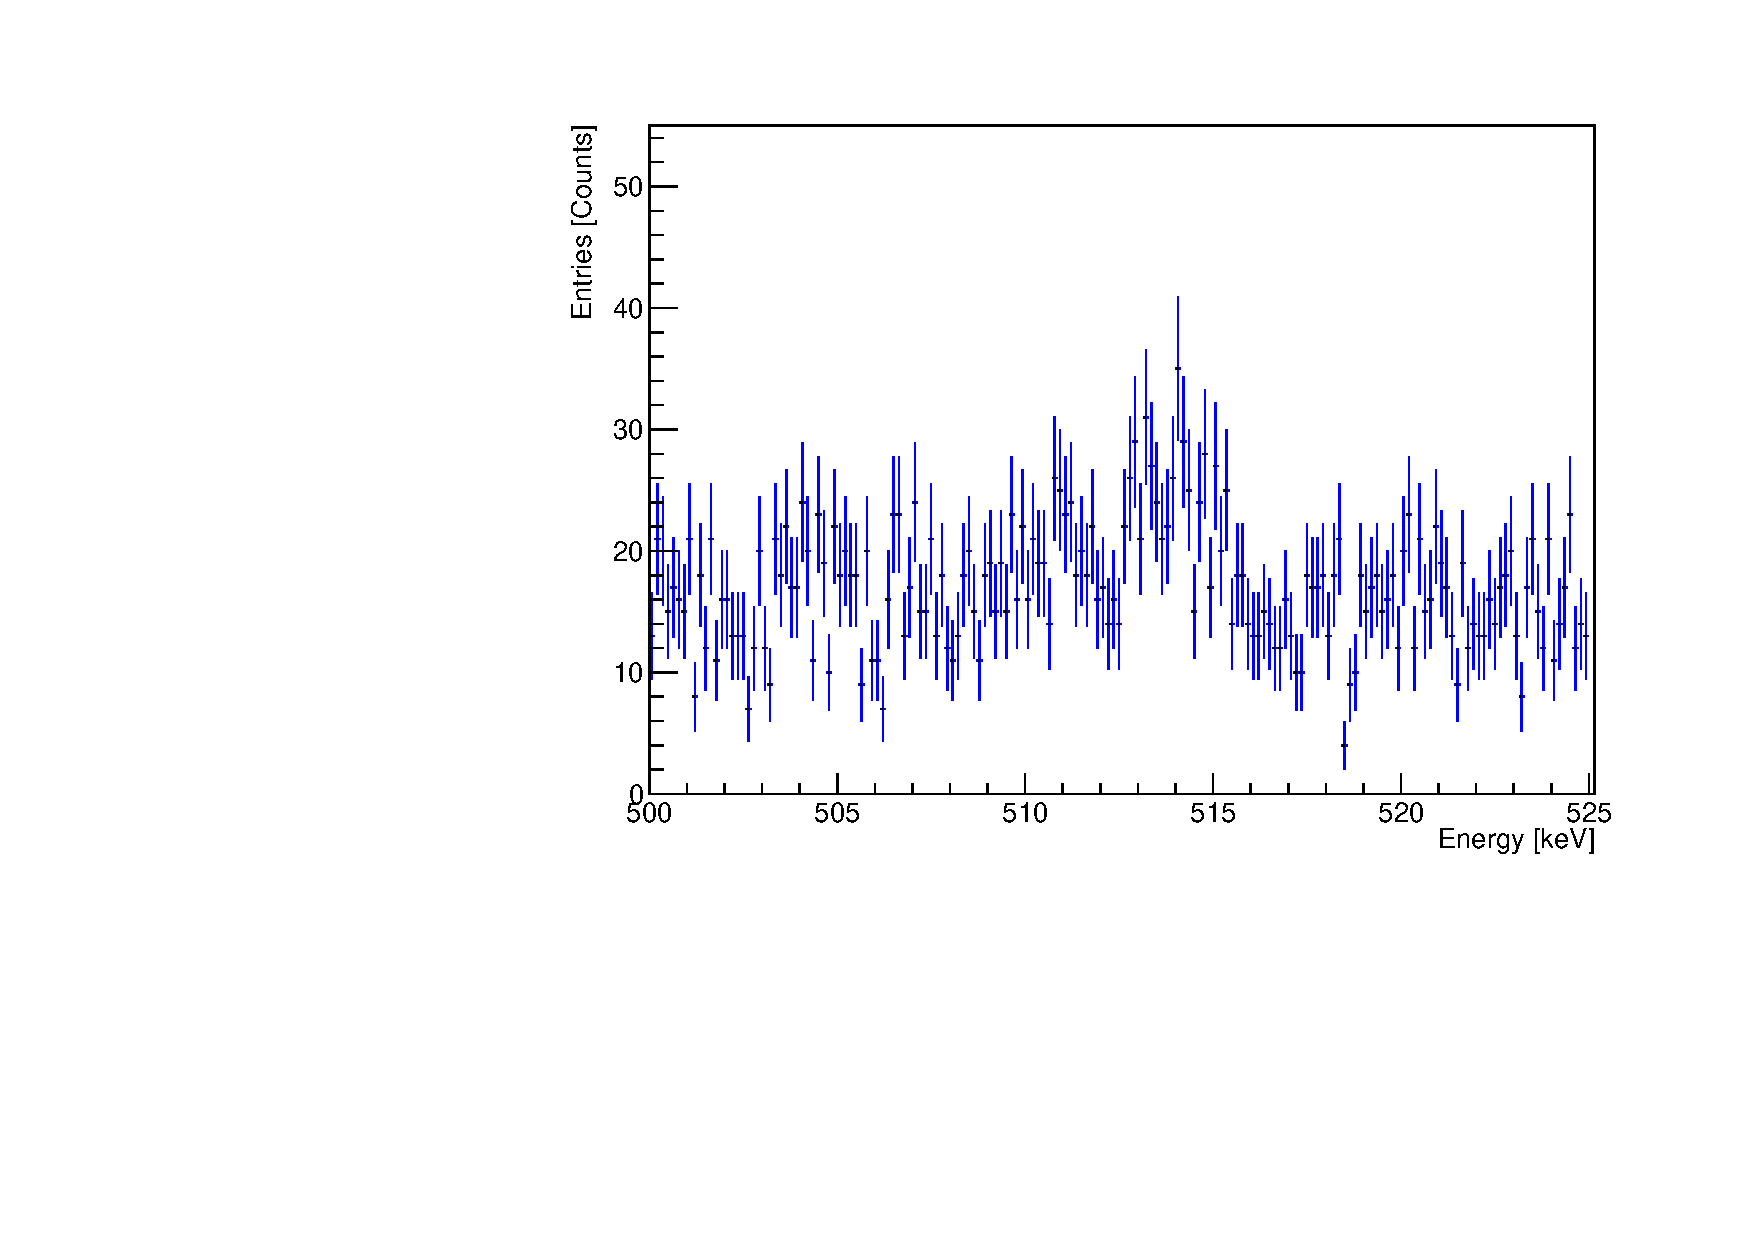
\includegraphics[width=75mm]{./Bilder/500525NoFilterBEGes.pdf}
  \label{fig:NoFilterBEGes}
  \caption{BEGes}
\end{subfigure}%
\begin{subfigure}{.5\textwidth}
  \centering
	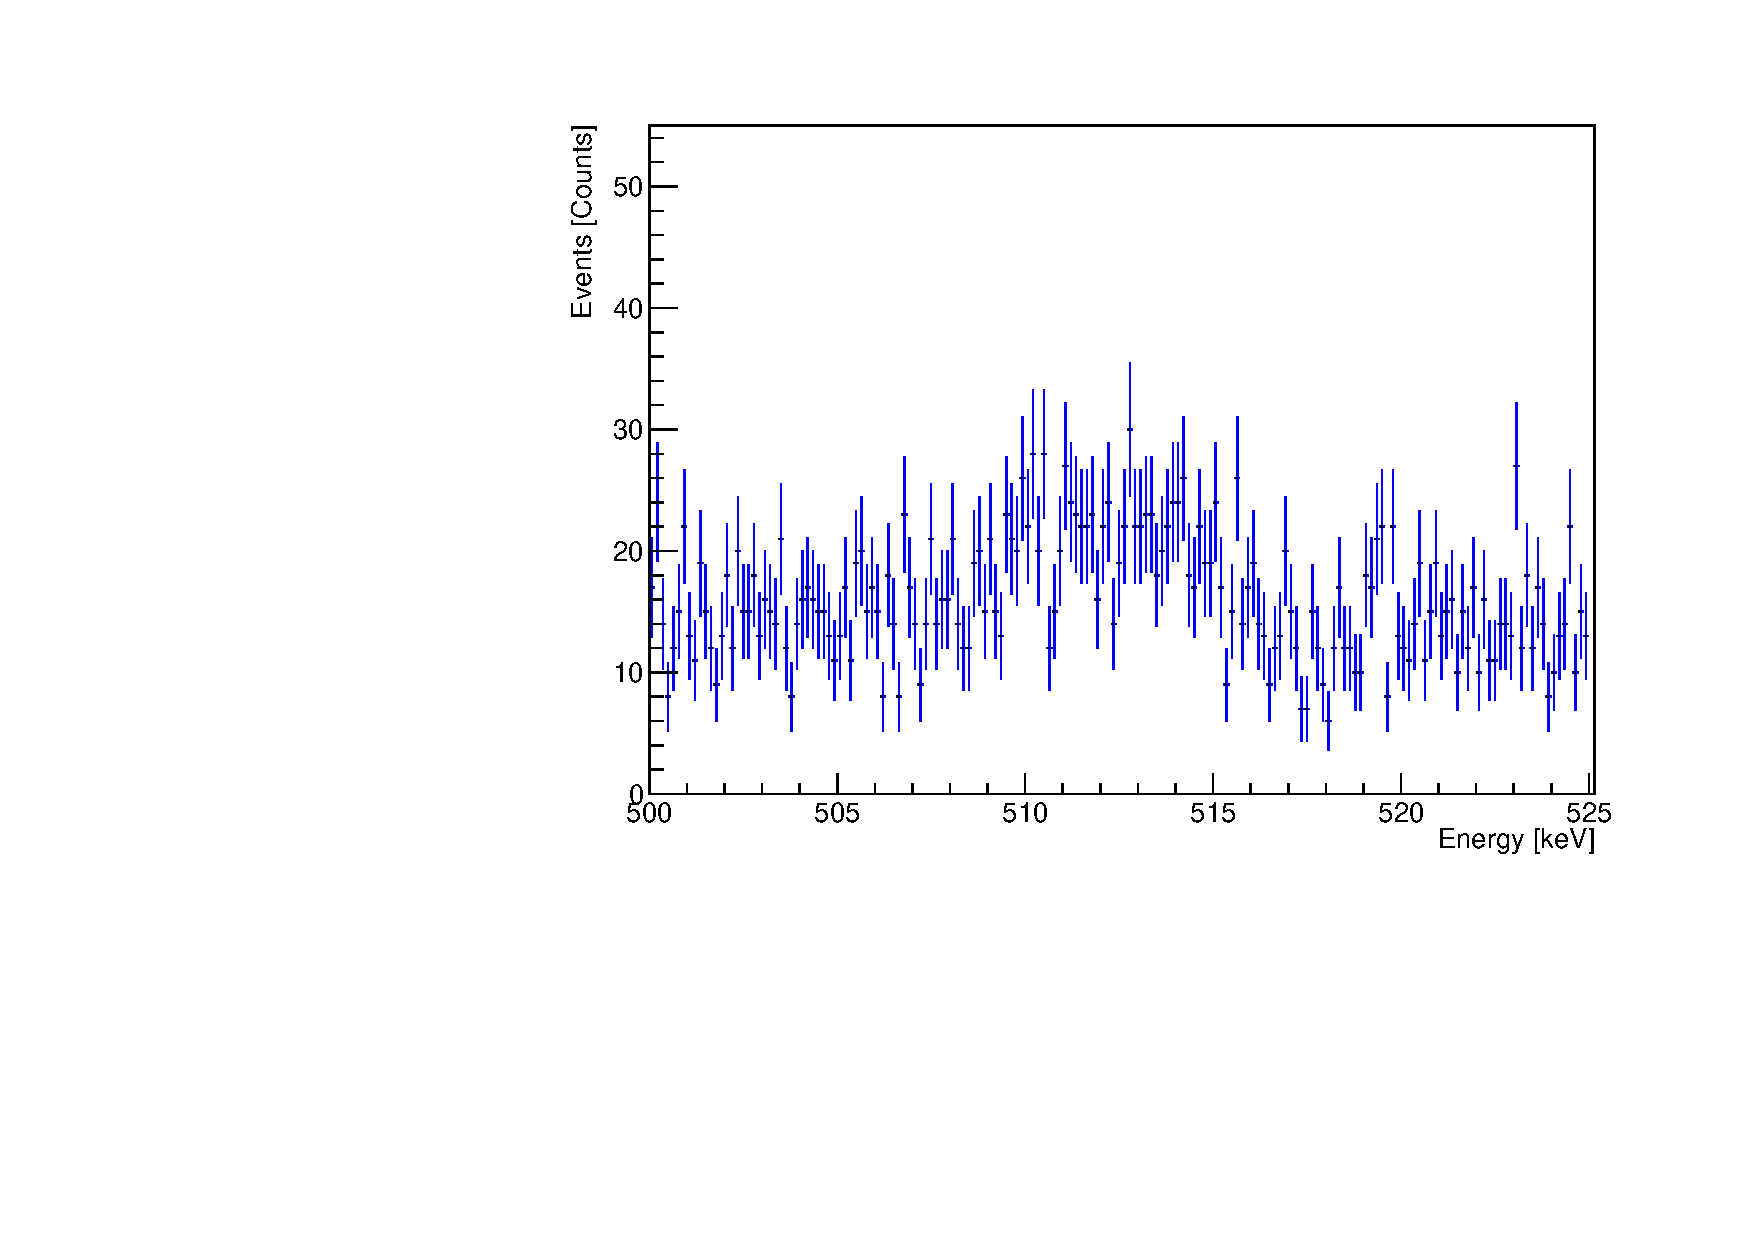
\includegraphics[width=75mm]{./Bilder/500525NoFilterCOAX.pdf}
  \caption{COAX}
  \label{fig:NoFilterCOAX}
\end{subfigure}
    \\
	\vspace{0.5cm}
	\caption{All events measured by the respective detectors in the range of 500keV to 525keV.}
\end{figure}

Now that we have the two spectra of the corresponding detectors, we have two possible ways of how we can determine the number of measured events around the 514keV peak.
The easier way is to just use the spectra as they are and only change the used fit function so that it also takes the second peak into account when fitting.
Another possible approach tries to suppress the annihilation peak and then fit the spectrum with only one Gaussian peak.
This can hopefully be done by using the liquid argon veto of GERDA and the precoincidence of the electron scintillation in the photomultipliers. 
\\ 

In this theses we will try to go both ways separately and later compare their resulting values.
We will probably end up using the unsuppressed spectra to determine the amount of events measured and only use the other method as a crosscheck.
As we will see later this is because the used filter also filters out events from the 514keV line peak.
This results in a lower amount of events measured at this energy and therefore, in the end, gives us a lower activity than there is in actuality. 
But to understand why this filter also filters out these false positives we have to discuss how this filter works first.
This will be the topic of the following section.
\\

\section{Annihilation Peak Suppression}
\label{sec:APS}

As mentioned above, it should be theoretically possible to filter out the majority of the positron electron annihilation events by using the scintillation property of the liquid argon.
In the case of the \Kr decay into the excited \nuc{Rb}{85m} the emitted electron has a very low mean kinetic energy of E\(_{mean}=47.65\)keV.
!!!!! hier die abgeschätzte Anzahl an Photonen angeben !!!!!
This means that in the majority of these decays no light should be seen in the detectors, because the low amount of photons are unlikely to trigger any of them.
In contrast to that you can expect a very strong light signal every time a positron electron annihilation occurs. 
One should therefor be able to filter out almost all of the annihilation events while keeping the majority of the \Kr decay by only using events where this flag is not triggered.
This chapter tries to implement a filter that uses this mechanism and discusses in the end how successful the repression really was.
\\

Among other things, each event in tier 4 was given a flag called "isLArVetoed".
This flag is always triggered whenever an event in the Germanium detectors coincides with a scintillation signal of at least 0.5phe in one of the photomultipliers positioned in the liquid argon tank \cite{agostini_background_2017}.
If one plots all events in which this flag has not been set one gets figure \ref{fig:LArBEGes} for the BEGes and figure \ref{fig:LArCOAX} for the COAX detectors.
You can see that the positron electron annihilation peak can not be identified any longer while the 514keV peak seems almost unchanged.
\\

\begin{figure}[t!]
\centering
\begin{subfigure}{0.5\textwidth}
	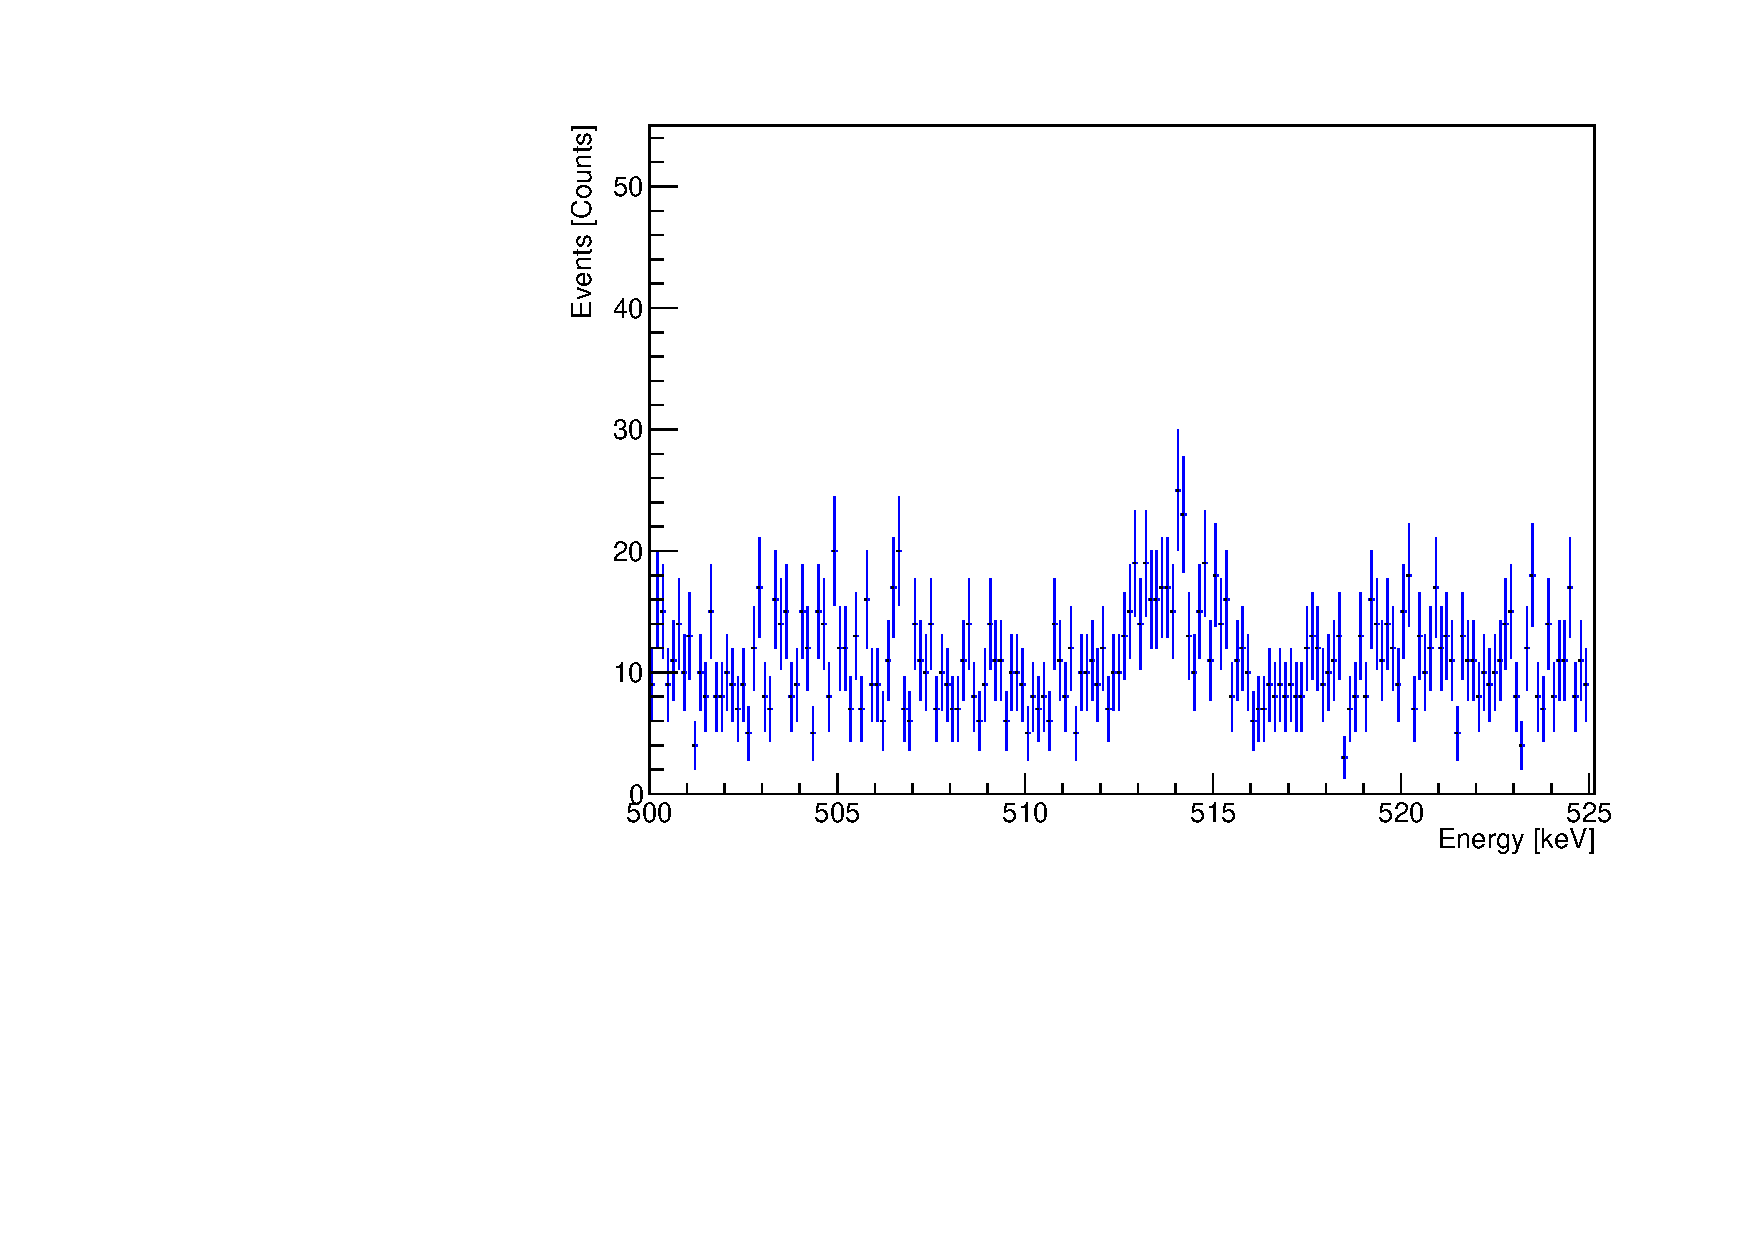
\includegraphics[width=75mm]{./Bilder/500525LArVetoBEGes.pdf}
    \caption{BEGes}
  \label{fig:LArBEGes}
\end{subfigure}%
\begin{subfigure}{0.5\textwidth}
	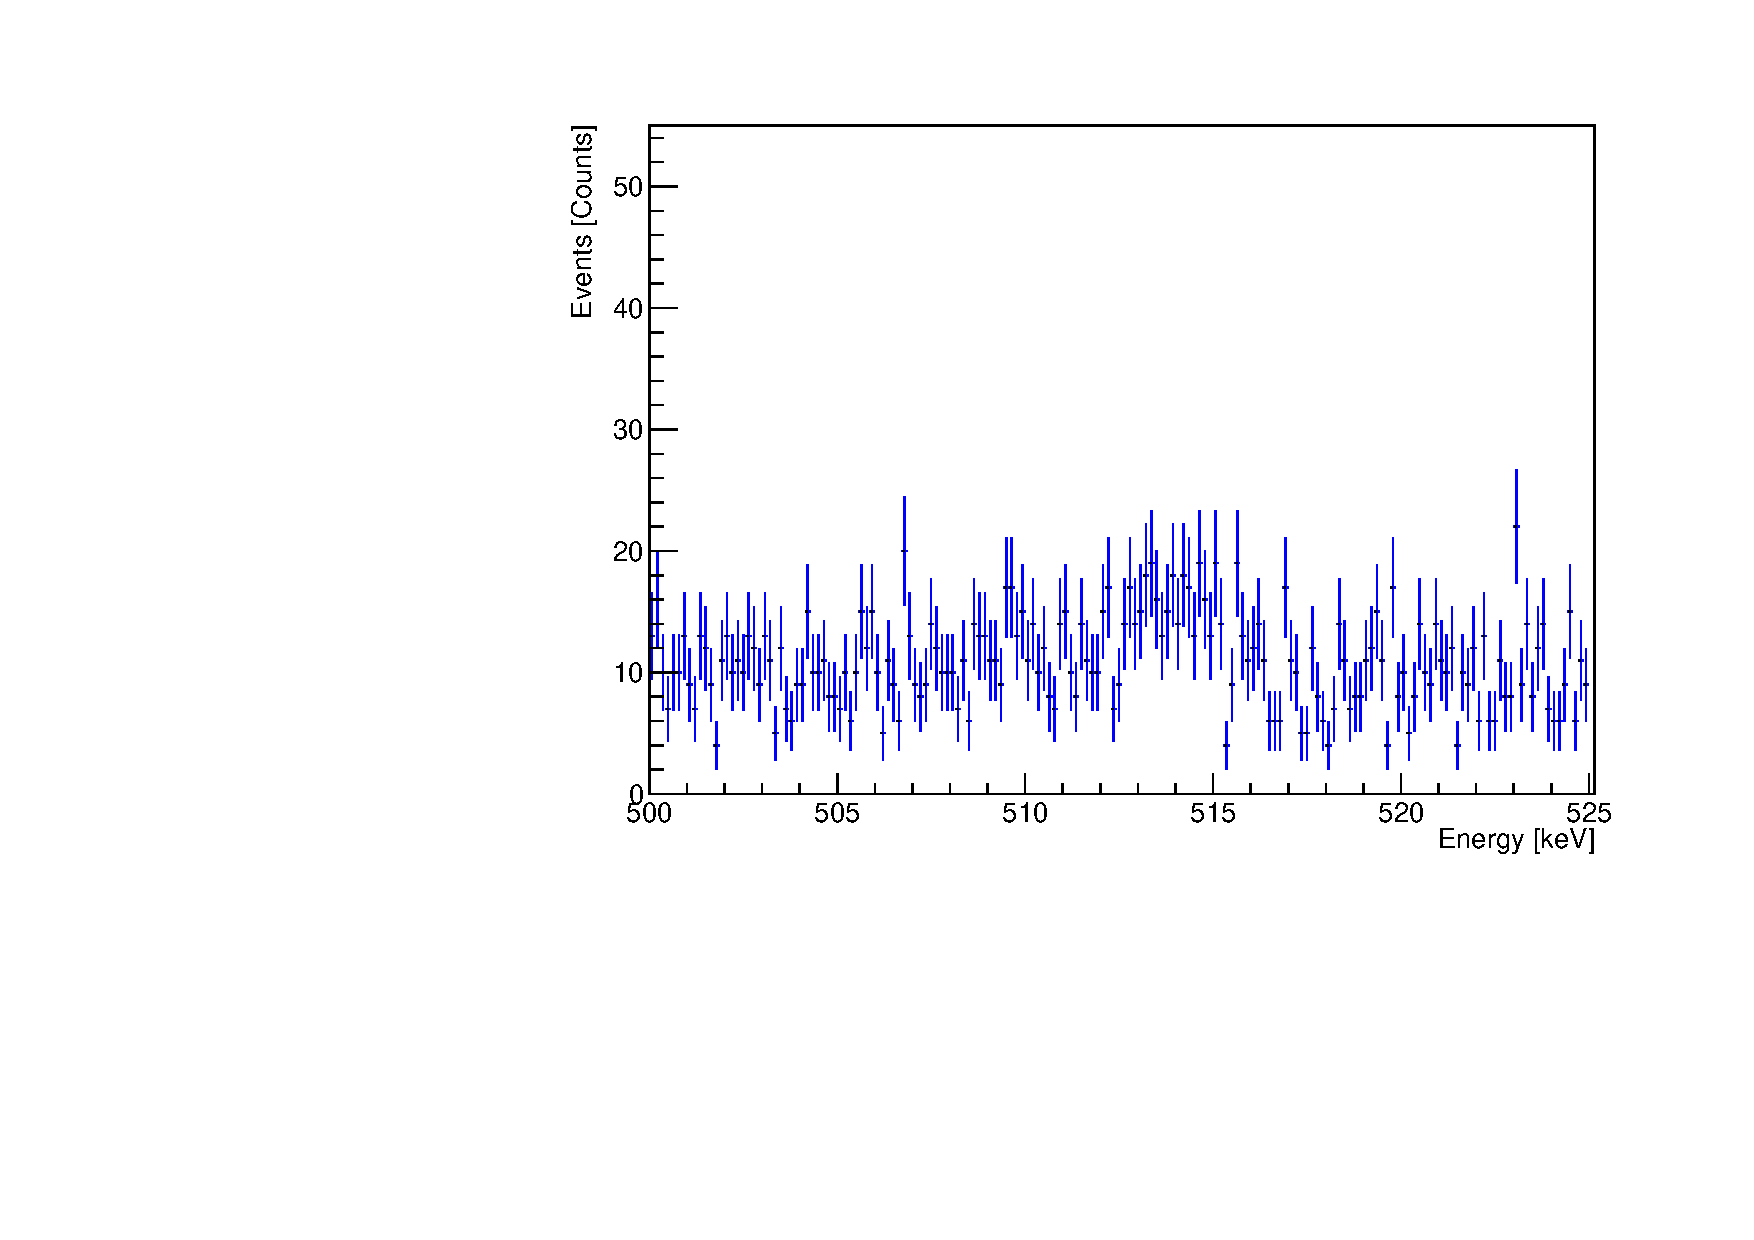
\includegraphics[width=75mm]{./Bilder/500525LArVetoCOAX.pdf}
  \caption{COAX}
  \label{fig:LArCOAX}
\end{subfigure}
    \\
	\vspace{0.5cm}
    \caption{All events measured by the respective detectors with the LAr filter applied in the range of 500keV to 525keV.}
\end{figure}

\begin{figure}[t!]
	\centering
	\begin{subfigure}{.5\textwidth}
		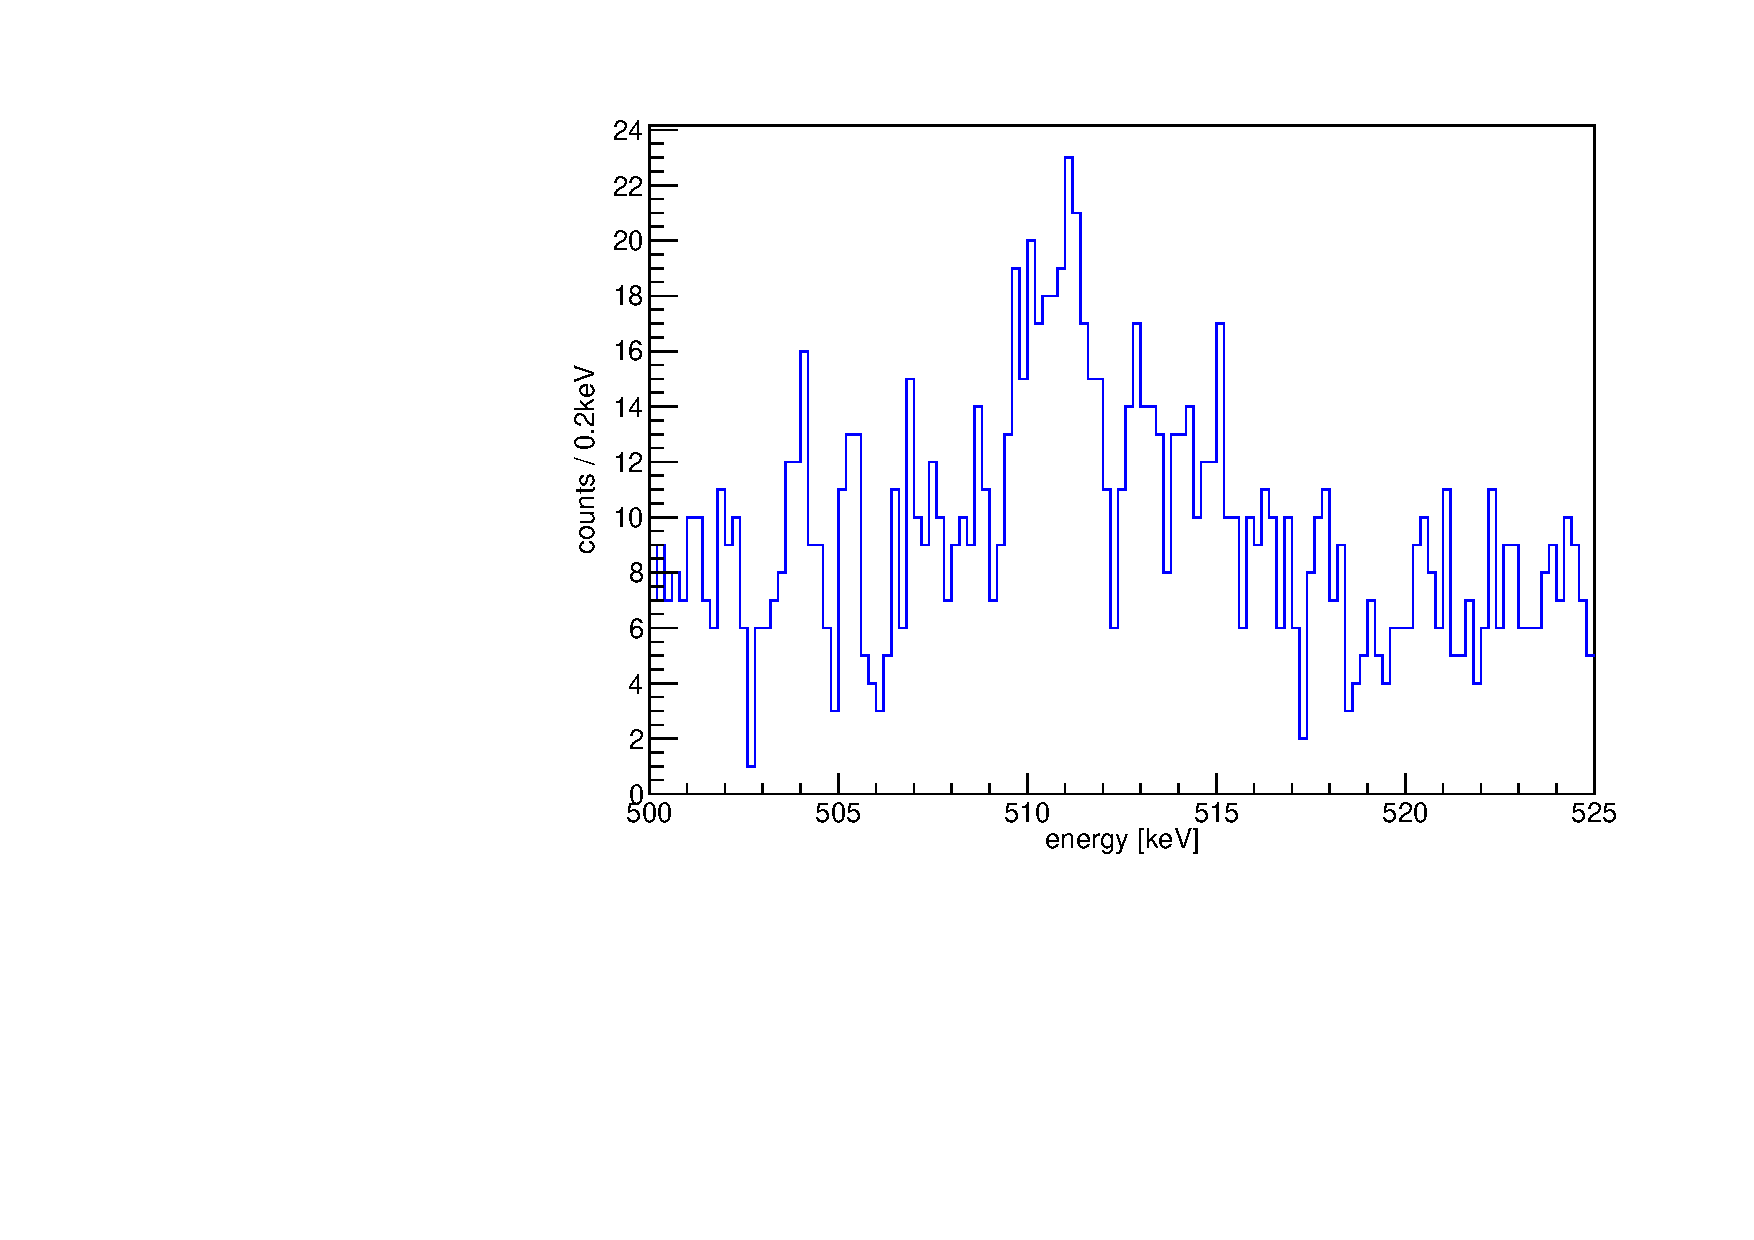
\includegraphics[width=75mm]{./Bilder/AntiLArBEGe.pdf}
		\caption{BEGes}
		\label{fig:AntiLArBEGes}
	\end{subfigure}%
	\begin{subfigure}{.5\textwidth}
		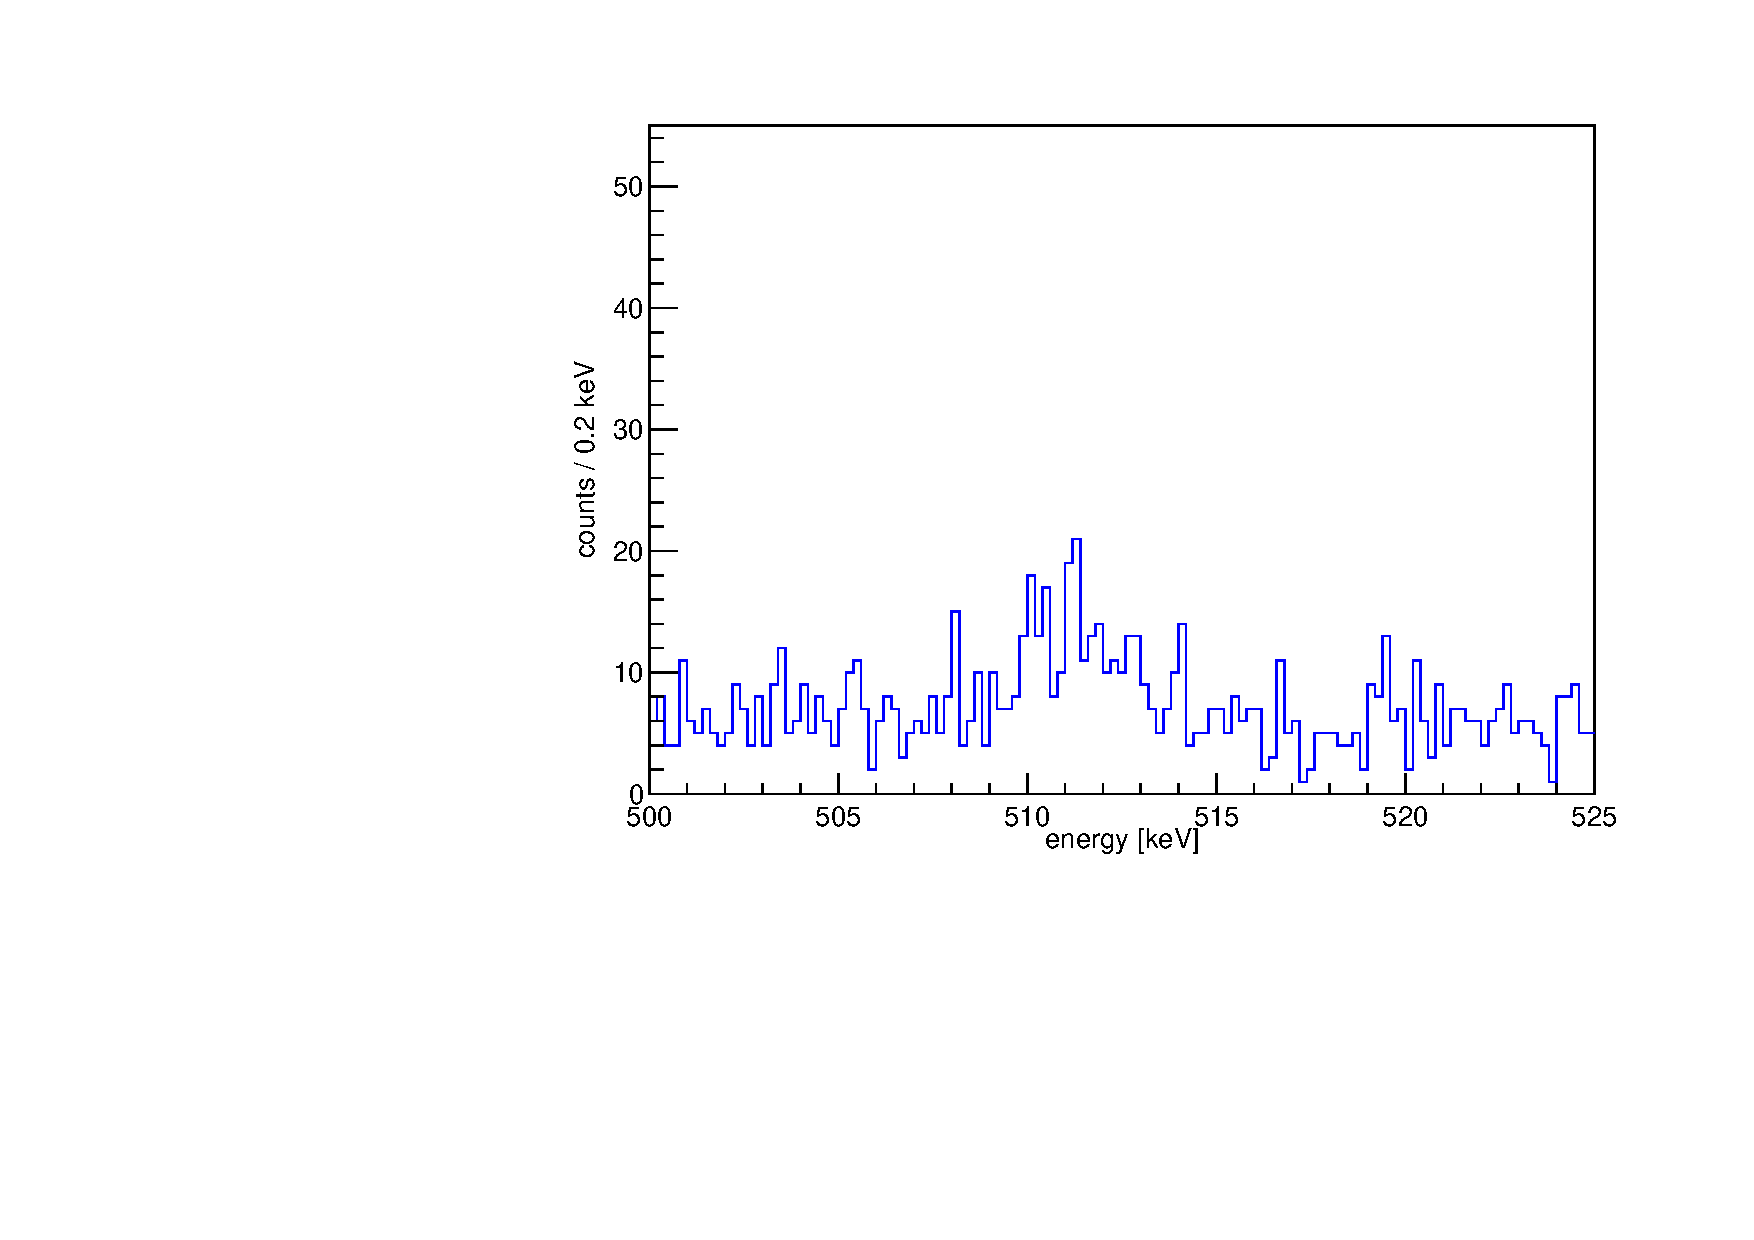
\includegraphics[width=75mm]{./Bilder/AntiLArCOAX.pdf}
		\caption{COAX}
		\label{fig:AntiLArCOAX}
	\end{subfigure}
	\\
	\vspace{0.5cm}
	\caption{All events measured by the respective detectors with the LAr filter applied in the range of 500keV to 525keV.}
\end{figure}

In comparison, when you take only those events in which the liquid argon veto was triggered you get figure \ref{fig:AntiLArBEGes} and \ref{fig:AntiLArCOAX}.
From those you can see that the majority of not background events that got filtered out have an energy around the 511keV.
But one can already see that there are also a small deviation from the background level around the 514keV marks.
This means that some of events caused by \Kr decays must have also triggered the liquid argon veto.
\\

It is therefor of interest to investigate how many of the \Kr decay caused events were filtered out by accident and whether it is possible to recover them.
The absolute number of events filtered out by the liquid argon veto in the energy range of 509 to 519 keV is 1728.
This number is way too big to look at every individual case.
\\

Luckily we can use the fact that the excited \nuc{Rb}{85m} state has a half life of 1.015 \(\unit{\mus}\).
This means that theoretically we should be able to measure a pre-coincedence event of the beta creating scintillation light which can then be measured before even a signal in the germanium detectors could be seen.
This way we can hopefully identify the majority of events created by \Kr decays from the rest of the filtered signals.
To do this, we have to limit the events used for our investigation to those events that have a negative time difference between these two events respective to the Germanium detector signal.
The time difference for each individual liquid argon events is already analyzed and stored in the vector $"$triggerLAr$"$ of the tier 3 data set.
This vector has the same number of dimensions as there are photomultipliers and every entry is indexed with the corresponding input channel of the respective photomultiplier.
The entries of this vector are again vectors themselves storing the time difference for every signal that triggered the liquid argon veto in the corresponding channel.
Since the events are listed in ascending order and we are interested in the first trigger event of the photomultiplier, we use only the first entry of this inner vector here for simplicity reasons.
From now on we only use events in which at least one photomultiplier measured a negative time difference.
\\

In addition, we also know that the energy of the released beta electron is relatively low.
This means that we can expect that only a small number of photomultipliers will measure a signal of a \Kr decay if any at all.
In the case of a measured signal we will only use those events that have a maximum of four different triggered photomultipliers.
Allowing events with a maximum of four different triggered photomultipliers is already a lot for a \Kr decay. 
But we wanted to do a more detailed manually investigation later anyways which is why the filter can be a little coarser here.
\\

\begin{figure}[t!]
	\centering
	\ifmakefigures%
	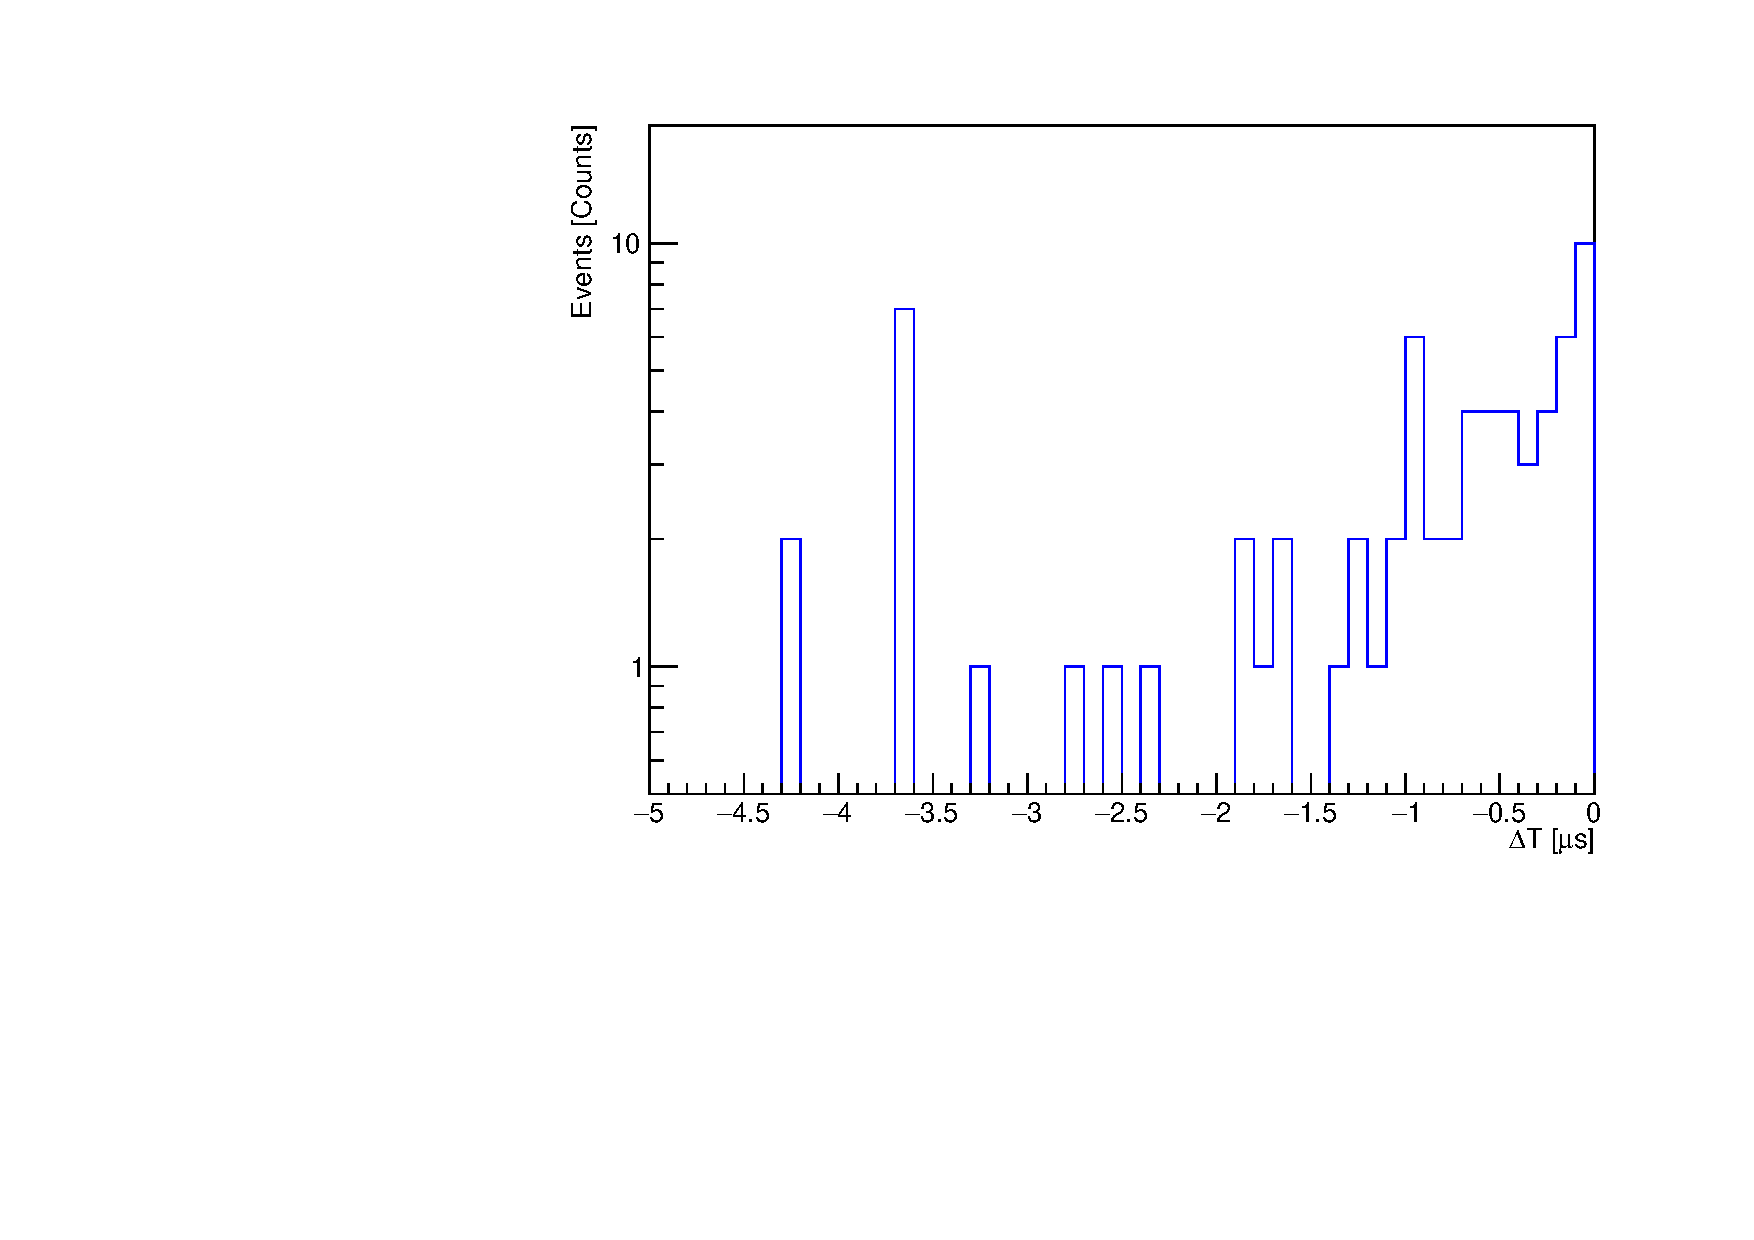
\includegraphics[width=100mm]{./Bilder/TriggerTimeOnly4.pdf}
	\fi%
	\label{fig:Trigger4}
	\caption{
		All liquid argon filtered events with a negative time difference between the event in the Germanium detector and a signal in the photomultipliers in the liquid argon tank.
	}
\end{figure}

If you apply these two restrictions to the liquid argon filtered events and only take those photomuliplier signals with a signal strength of at least 0.5 phe you get a distributions as seen in figure \ref{fig:Trigger4}.
We are only interested in the signals that measured at least 0.5 phe because, as mentioned above, this is the necessary intensity to trigger the LAr veto making them the signals of interest. 
The x axis is the time difference of the events in the photomultipliers from the signal measured in one of the Germanium detectors.
Theoretically it should now be possible to see a exponential increase from the negative scale towards a vanishing time difference.
But because of the small number of events however, it is almost impossible to make any statements about the course of these events.
\\

!!!!! diesen Teil noch Überarbeiten wenn nicht weglassen !!!!!

Interestingly, the majority of all signals with a negative time difference were measured by the PMTs. 
This could perhaps be due to the better temporal resolution of the PMTs. 
The signals of all PMTs are recorded with a resolution of 10ns and the SiPM with a resolution of 80ns but over a larger range than the PMTs \cite{agostini_background_2017}. 
However, since the expected time difference is in the order of \(\mu\)s, this is no reason for the reduced number of measured events. 
Another difference between the photomultiplier types is that the PMTs have a faster reaction time than the SiPMs. 
As we will see, practically all deflections in the measured intensity of the PMT signal caused by procoincedents have already subsided before the signal was measured in the germanium detectors. 
Thus a clear maximum should be recognizable before the germanium detector events.
In contrast, the measured signal of the SiPMs increases exponentially with a characteristic time in the order of 10\(\mu\)s. 
The trigger positions are then determined by software. 
However, this should still be able to determine the trigger position of the signals for procoincedence events with sufficient accuracy.
!!!!! Hier dir noch was genaueres ausdenken, wenn überhaupt !!!!!
\\

!!!!! bis hier hin !!!!!

Nevertheless we were able to lower the number of potential 514keV photons from \Kr decay events from 1728 down to only 55.  
These remaining events can now be manually examined with a software called GerLa written by GERDA employees.
This tool allows you to search for a specific event and see all recorded signals of the Germanium detectors and the photomultipliers around the time frame of this event.
\\

With this program one can now perform a manual filter by looking at the remaining 55 events individually and perform a specific procedure to determine whether they are signals from a \Kr decay or not.
This procedure consists of filtering out every event that has a combined light intensity of over 5 phe and every event that only has a negative time difference in a signal weaker than 0.5 phe.
The upper limit of the light intensity comes from the fact that the mean kinetic energy of the electron released from the decay is 47.65keV. 
With the luminosity of liquid argon of about 50 photons/MeV one can expect about 2.5 photons at these energies. 
It can then be assumed that the predominant part of all betas released in the investigated decay only emit 5 photons at best.
\\

\begin{figure}[t!]
	\centering
	\ifmakefigures%
	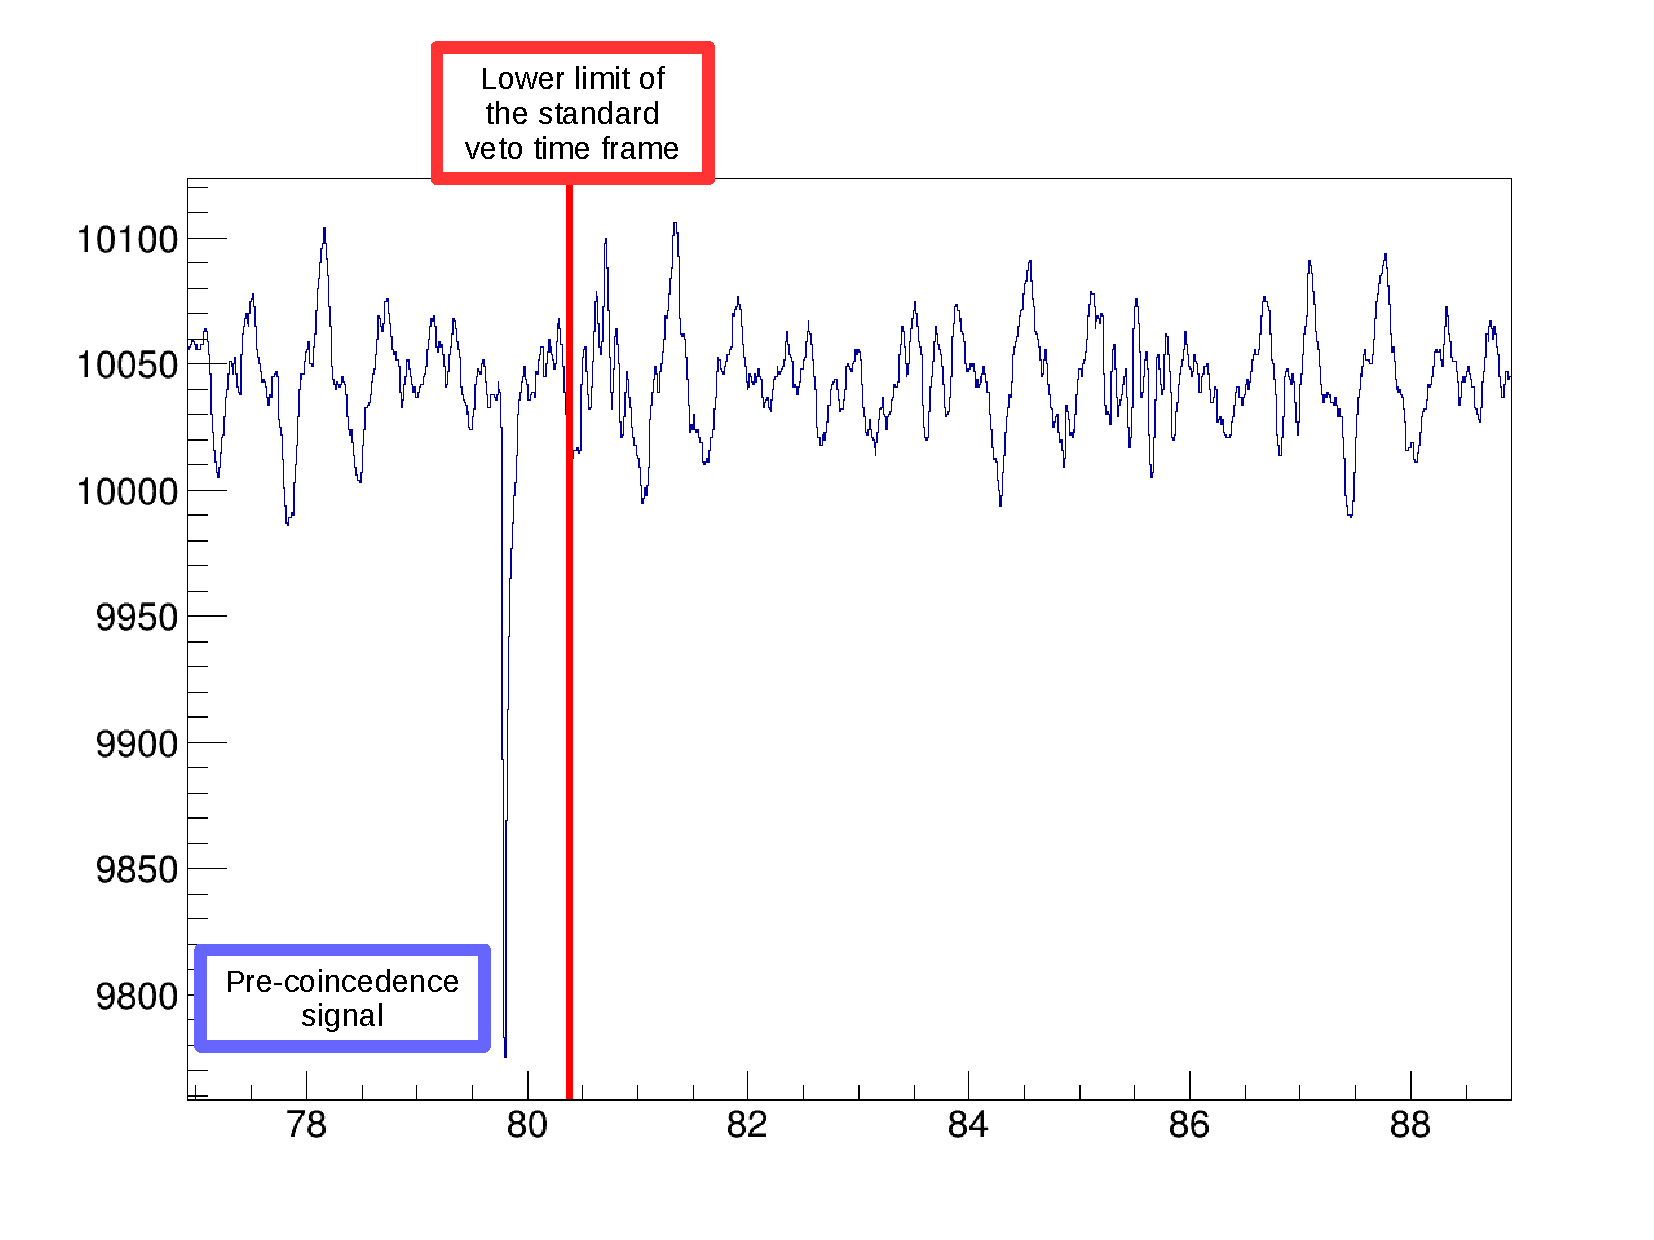
\includegraphics[width=100mm]{./Bilder/BeispielSignal.pdf}
	\fi%
	\label{fig:Trigger4}
	\caption{
    The recorded signal of the photomultiplier tube P4 from the event with event number 1614036. !!!!!Hier noch was zu den Achsen!!!!!. 
    The blue bar represents the moment in time in which a signal in the Germanium detector was measured.
	}
\end{figure}

At this point we realized that this procedure does not really work as well as we hoped it would.
From the remaining 55 only a few events really were unambiguous enough that one could claim that they are the photons we expected.
After this much filtering we can assume that probably all of these events are in fact caused by a \Kr decays.
Signals like the one shown in figure \ref{fig:Trigger4} are a rare example of an almost model signal that we wanted to see.
The great majority of other events were either background events in the SiPM that randomly triggered the LAr veto or their measured signal was too strong.  
\\

With this it was now determined that the majority of events with a negative time difference are in fact not caused by a \Kr decay.
This means that the remaining \Kr decay events must have a positive time difference.
But it is practically impossible to recover them from there due to the great amount of individual events that have to be looked at.
Our recovery attempt has therefor failed.
\\

!!!!! DAS HIER IST AUCH NOCH EINE PROBLEMSTELLE !!!!!

Nevertheless we are still able to make some qualitative estimations about why approach did not work. 
When trying to make a more realistic estimation one can see qualitatively that the actual portion of recovered events must be smaller.
An important factor limiting this recovery rate originates from an estimation applied in this approach.
It was approximated that the electrons created scintillation light instantaneously after being released.
In reality, the moment an electron emits scintillation light is determined by many complex mechanisms. 
However, its behavior can be approximated by a relaxation approach. 
This gives you a new characteristic time with which you can describe how many electrons have already created scintillation light after what time. 
But this not spontaneous behavior means, that the measured signal depends on both the relaxation time of the \nuc{Rb}{85} and the scintillation light of the electron.
It is therefor quite possible, that a number of \Kr decay events can have a positive effective time difference.
Those are then lost in our analysis due to us filtering out every event that has a positive time difference.
This results in a lower recovery rate.
\\

Now that we have seen that we were not able to recover any of the falsely filtered \Kr caused events it is justified to also question whether the majority of the rare \Kr decays can even pass through the liquid argon filter itself.
But we only get a satisfactory answer with a quantitative analysis which will be performed in the following chapter.
\\

\section{Fitting}
\label{sec:Fitting}

Our strategy to calculate the activity of \Kr through the 514keV peak involves determining the absolute amount of measured \Kr decays events over all of \PII.
Due to the still enormous amount of events from other sources that can not be suppressed, for example the \nuc{Ge}{76} decays, it is necessary to fit the 514keV peak with a suitable fit function.
The amount of measured \Kr decay events can then be calculated by integrating over the found fit function and dividing by the probability of the specific decay into \nuc{Rb}{85m}.
\\

The not liquid argon filtered spectrum \ref{fig:NoFilterBEGes} and \ref{fig:NoFilterCOAX} show two peaks.
This requires the fit function to include two Gaussian functions from which only the parameters of the second peak will then be analyzed.
Additionally to the two Gaussian peaks a constant and an exponential background function will be added.
When looking at the not liquid argon filtered spectra again we can see that over the course of the displayed interval no real change in count rate over energy can be seen (see figure \ref{fig:NoFilterBEGes} and \ref{fig:NoFilterCOAX}).
But theoretically we expect the distribution of the germanium events to behave like its phase-space function and therefor change with energy.
It is therefor necessary to also consider this change in count rate over energy in the fit function.
The phase-space function of \nuc{Ge}{76} is very complex however.
In this case however is the energy interval relatively small compared to the complete spectrum of \nuc{Ge}{76}.
This allows the approximation that its phase-space function changes like an exponential decrease due to the general form of the measured spectrum in this energy range.
The resulting fit function is shown in equation \ref{equ:FitNoFilters}.
\\

\begin{equation}
\mathrm{f}(x) = \mathrm{A}\frac{1}{\sqrt{2\pi}\mathrm{C}}\exp\left(-\frac{(x-\mathrm{B})^2}{2\mathrm{C}^2}\right) + \mathrm{D}\frac{1}{\sqrt{2\pi}\mathrm{F}}\exp\left(-\frac{(x-\mathrm{E})^2}{2\mathrm{F}^2}\right) + \mathrm{G}\exp\left(\mathrm{H}x\right) + \mathrm{I}
\label{equ:FitNoFilters}
\end{equation}
\\

In the course of the fitting process it has to be mentioned that some fitness parameters have only been left free for rather small interval.
Most notably the values C and F, being the variances of two Gaussian peaks, were each only left free on a very small range around the values derived from the resolutions of the detectors at their specific energies (see appendix section \ref{sec:ResDetermination}).
When you apply the fit function to the two different spectra of the two kinds of detectors you get the graphs displayed in figure \ref{fig:FitNoFilterBEGes} and \ref{fig:FitNoFilterCOAX}.
The resulting fit parameters are listed in table \ref{tab:FitParNoFilter}. 
\\

\begin{figure}[t!]
	\centering
	\begin{subfigure}{.5\textwidth}
		\centering
		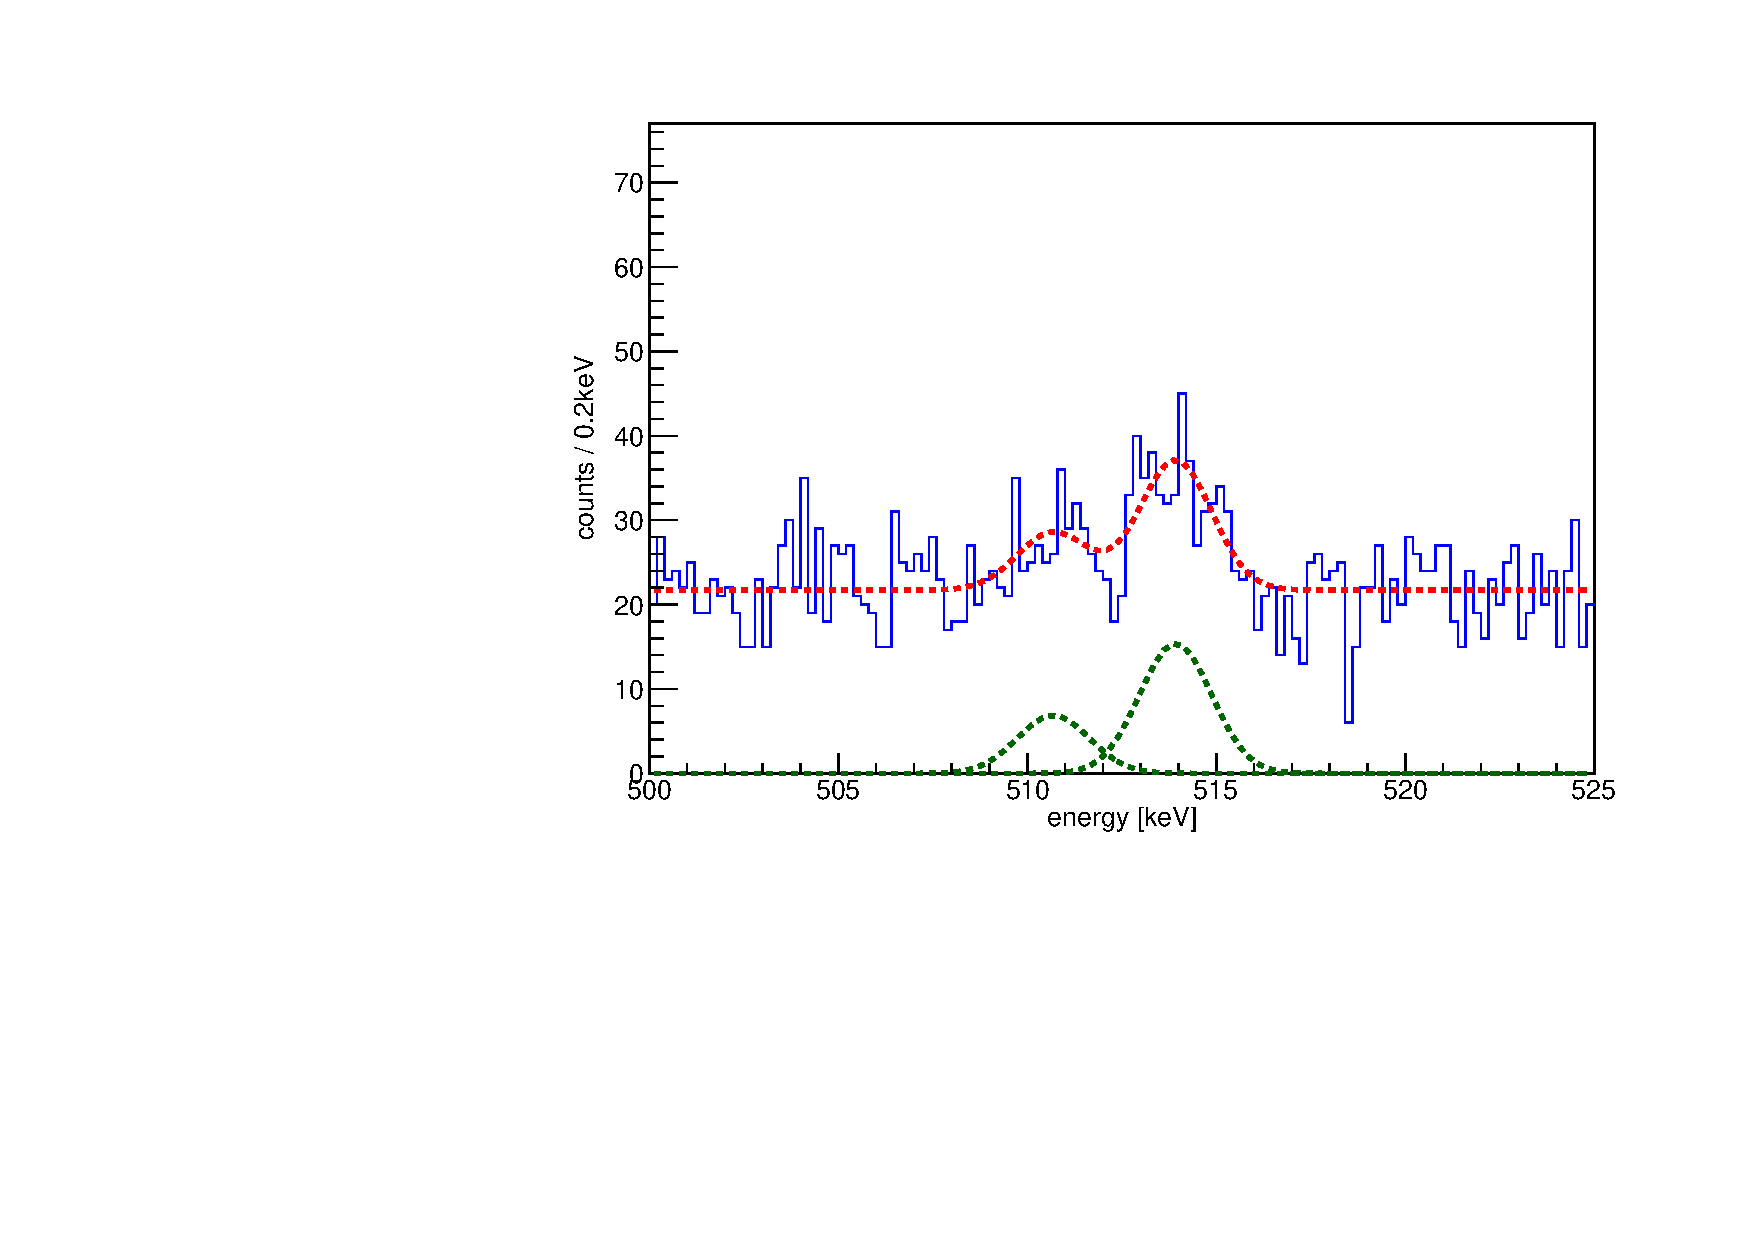
\includegraphics[width=75mm]{./Bilder/500525FitNoFilterBEGes.pdf}
		\caption{BEGes}
		\label{fig:FitNoFilterBEGes}
	\end{subfigure}%
	\begin{subfigure}{.5\textwidth}
		\centering
		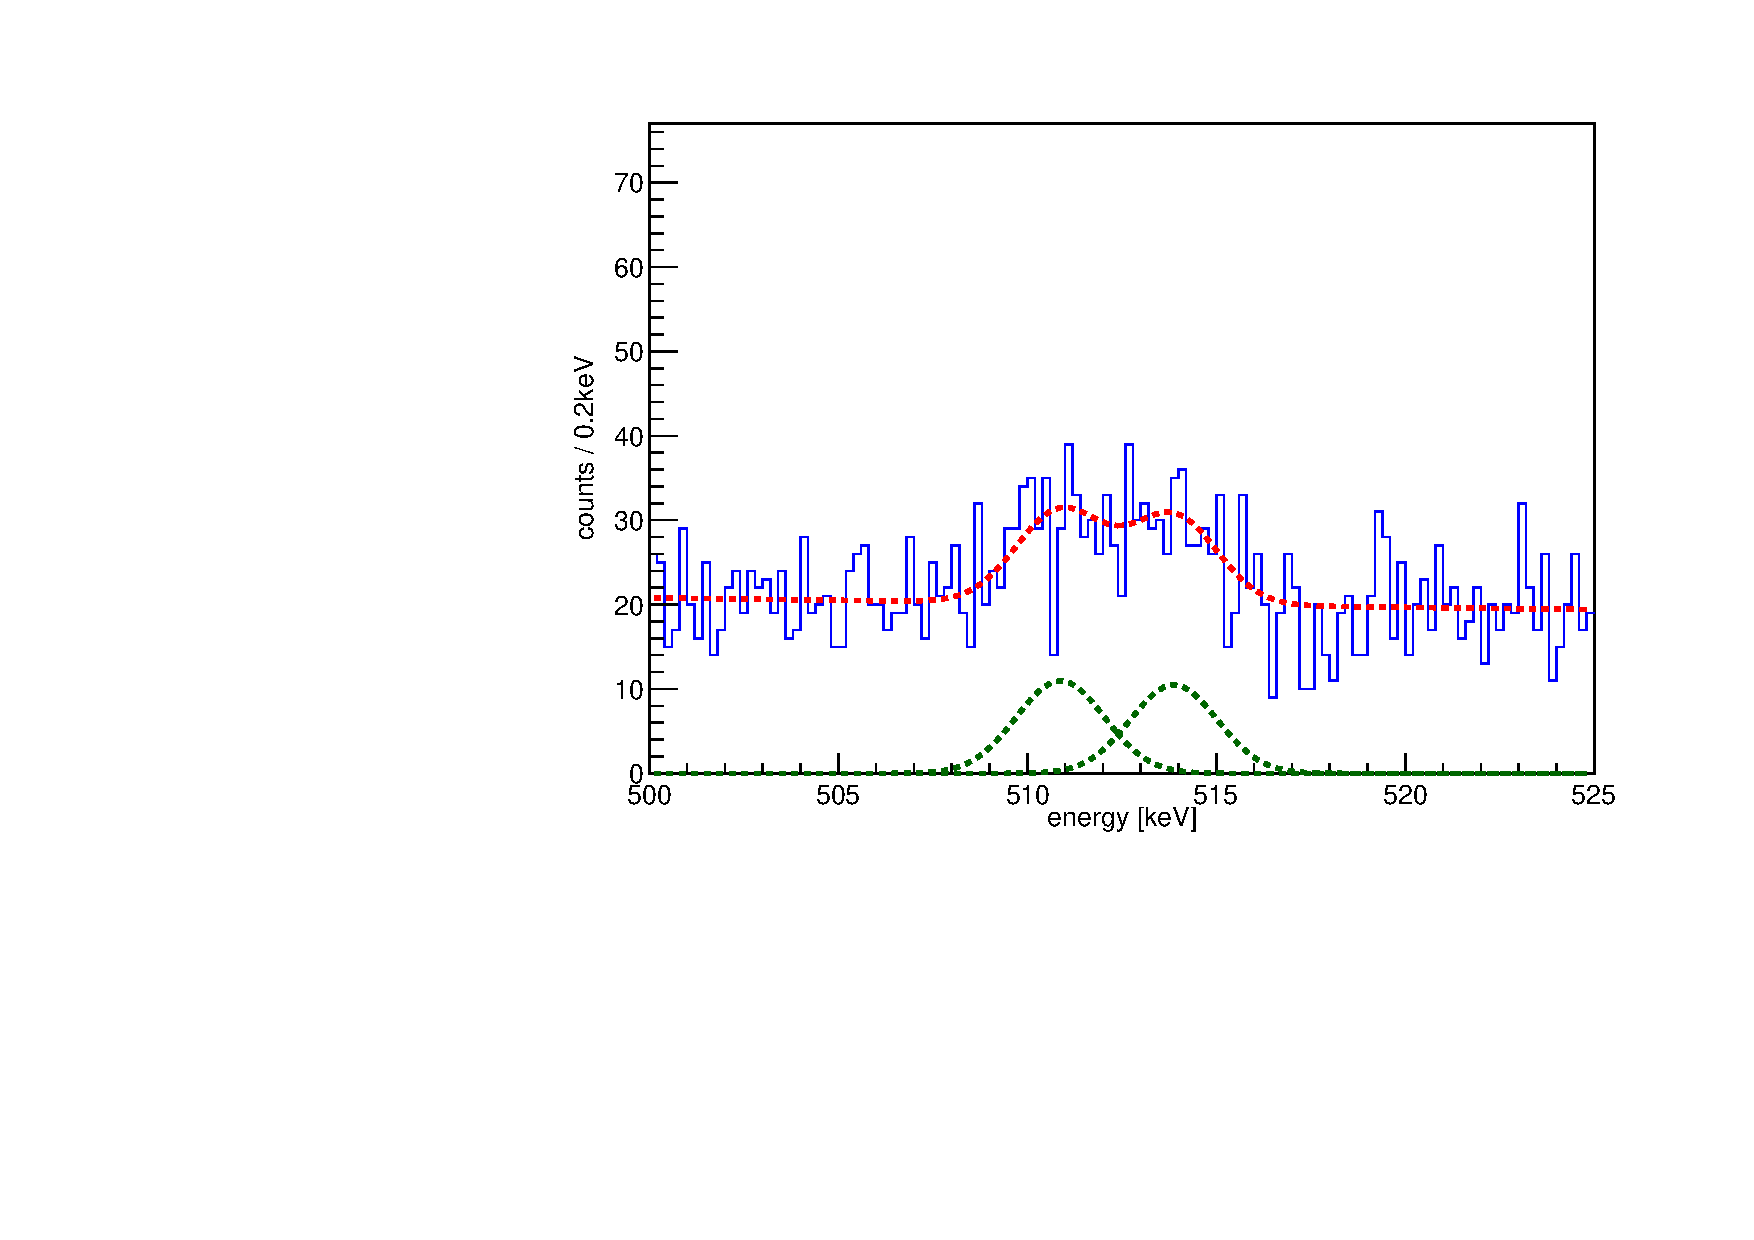
\includegraphics[width=75mm]{./Bilder/500525FitNoFilterCOAX.pdf}
		\caption{COAX}
		\label{fig:FitNoFilterCOAX}
	\end{subfigure}
    \\
	\vspace{0.5cm}
	\caption{All events measured by the respective detectors in the range of 500keV to 525keV fitted with a fit function in the form seen in equation \ref{equ:FitNoFilters}. The green function represent the two Gaussian peaks independently using the determined fit parameters.}
\vspace{0.5cm}
\end{figure}
\\

\begin{figure}[t!]
\centering
\begin{tabular}{|c|c|c|}
\hline
Name	& Value [BEGes] & Valuse [COAX]\\ 
\hline
A  &	(16.384684 \(\pm\)	4.229890	)&	(29.842 \(\pm\)	3.968)	\\	
\hline
B  &	(510.689545  \(\pm\)	0.275479	)&	(510.750 \(\pm\)	0.265)\\	
\hline
C  &	(0.952063 \(\pm\)	0.010154	)	&	(1.564 \(\pm\)	0.236	)	\\
\hline
D  &	(36.757652 \(\pm\)	4.743389)	&	(20.463 \(\pm\)	3.279	)	\\
\hline
E  &	(513.923462 \(\pm\)	0.153953	)	&	(513.858 \(\pm\)	0.213)	\\
\hline
F  &	(0.952731 \(\pm\)	0.011750	)	&	(1.017 \(\pm\)	0.173	)	\\
\hline
G  &	(21.714308 \(\pm\)	0.432063)	&	(13.123 \(\pm\)	0.289	)	\\
\hline
H  &	(-224175.656250 \(\pm\)	0.000424)	&	(-384995.062 \(\pm\)	2.592)	\\
\hline
I  &	(-0.655847 \(\pm\) 0.399776)	&	(-40.573 \(\pm\)	1.414)\\
\hline

\end{tabular}
\label{tab:FitParNoFilter}
\captionof{table}[]{Fit parameters of fit function \ref{equ:FitNoFilters} applied on the spectra of the respective detectors.}
\end{figure}
\\



The only values of these fit parameters that is of real interest for the determination of the activity is variable D.
Its value is the amplitude of the second Gaussian peak.
Because the Gaussian peak was chosen in the normalized form this value also represents the amount of \Kr decays measured per binning of the histogram.
But we only want the amount of counts in the peak independently of the binning of the histogram.
We therefor have to multiply these values with $\frac{1}{0.2}\unit{keV}$.
Finally, we can conclude that in the BEGes an amount of !!!!! events was measured and in the COAX detectors a number !!!!! of events.
\\


From the fit parameter value H and I we can also see that as expected the change of the background over the inspected energy interval is neglactable.
Parameter I defines the change in energy and its value so small that the exponential function in the range that is investigated in has no real impact on the overall fit function.
But as mentioned before it would have been wrong to leave out the fit functions possibility to change over energy because otherwise it might have ruined our whole fitting process. 
\\


After finding the fit parameter for the not liquid argon filtered spectrum we now go to the filtered spectrum.
As mentioned above we can assumed that the positron electron annihilation peak is fully suppressed.
Additionally in the ideal case, that the majority of all \Kr decay events got through the liquid argon filter, we expect the amplitude of the Gaussian peak to be similar to the amplitude in the not liquid argon filtered case.
Therefor only one Gaussian peak has to be fitted together with the background function.
The fit results in the function displayed in equation \ref{equ:FitFilters}.
\\ 

\begin{equation}
\mathrm{f}(x) = \mathrm{A}\frac{1}{\sqrt{2\pi}\mathrm{C}}\exp\left(-\frac{(x-\mathrm{B})^2}{2\mathrm{C}^2}\right) + \mathrm{D}\exp\left(\mathrm{E}x\right) + \mathrm{F}
\label{equ:FitFilters}
\end{equation}
\\

After applying the fit to the spectra seen in figure \ref to \ref, you get the fit parameters displayed in table \ref.
As above, the amplitude A of the Gaussian peak correspond to the number of events measured in the area of the peak per binning.
This results in an amount of !!!! for the BEGe and !!!!! for the COAX spectrum.
As mentioned above these values are only planned to be a crosscheck for the not argon filtered values. 
Compared to those values, it can be seen that the number of events in the BEGe and in the COAX detectors has dropped considerably.
This means that some of the \Kr decay events must have been filtered out and a recovery of these falsely filtered \Kr decays is necessary.
But due to that not being possible we can not use those results in our analysis nor for a real crosscheck..
\\

\begin{figure}[t!]
	\centering
	\begin{subfigure}{.5\textwidth}
		\centering
		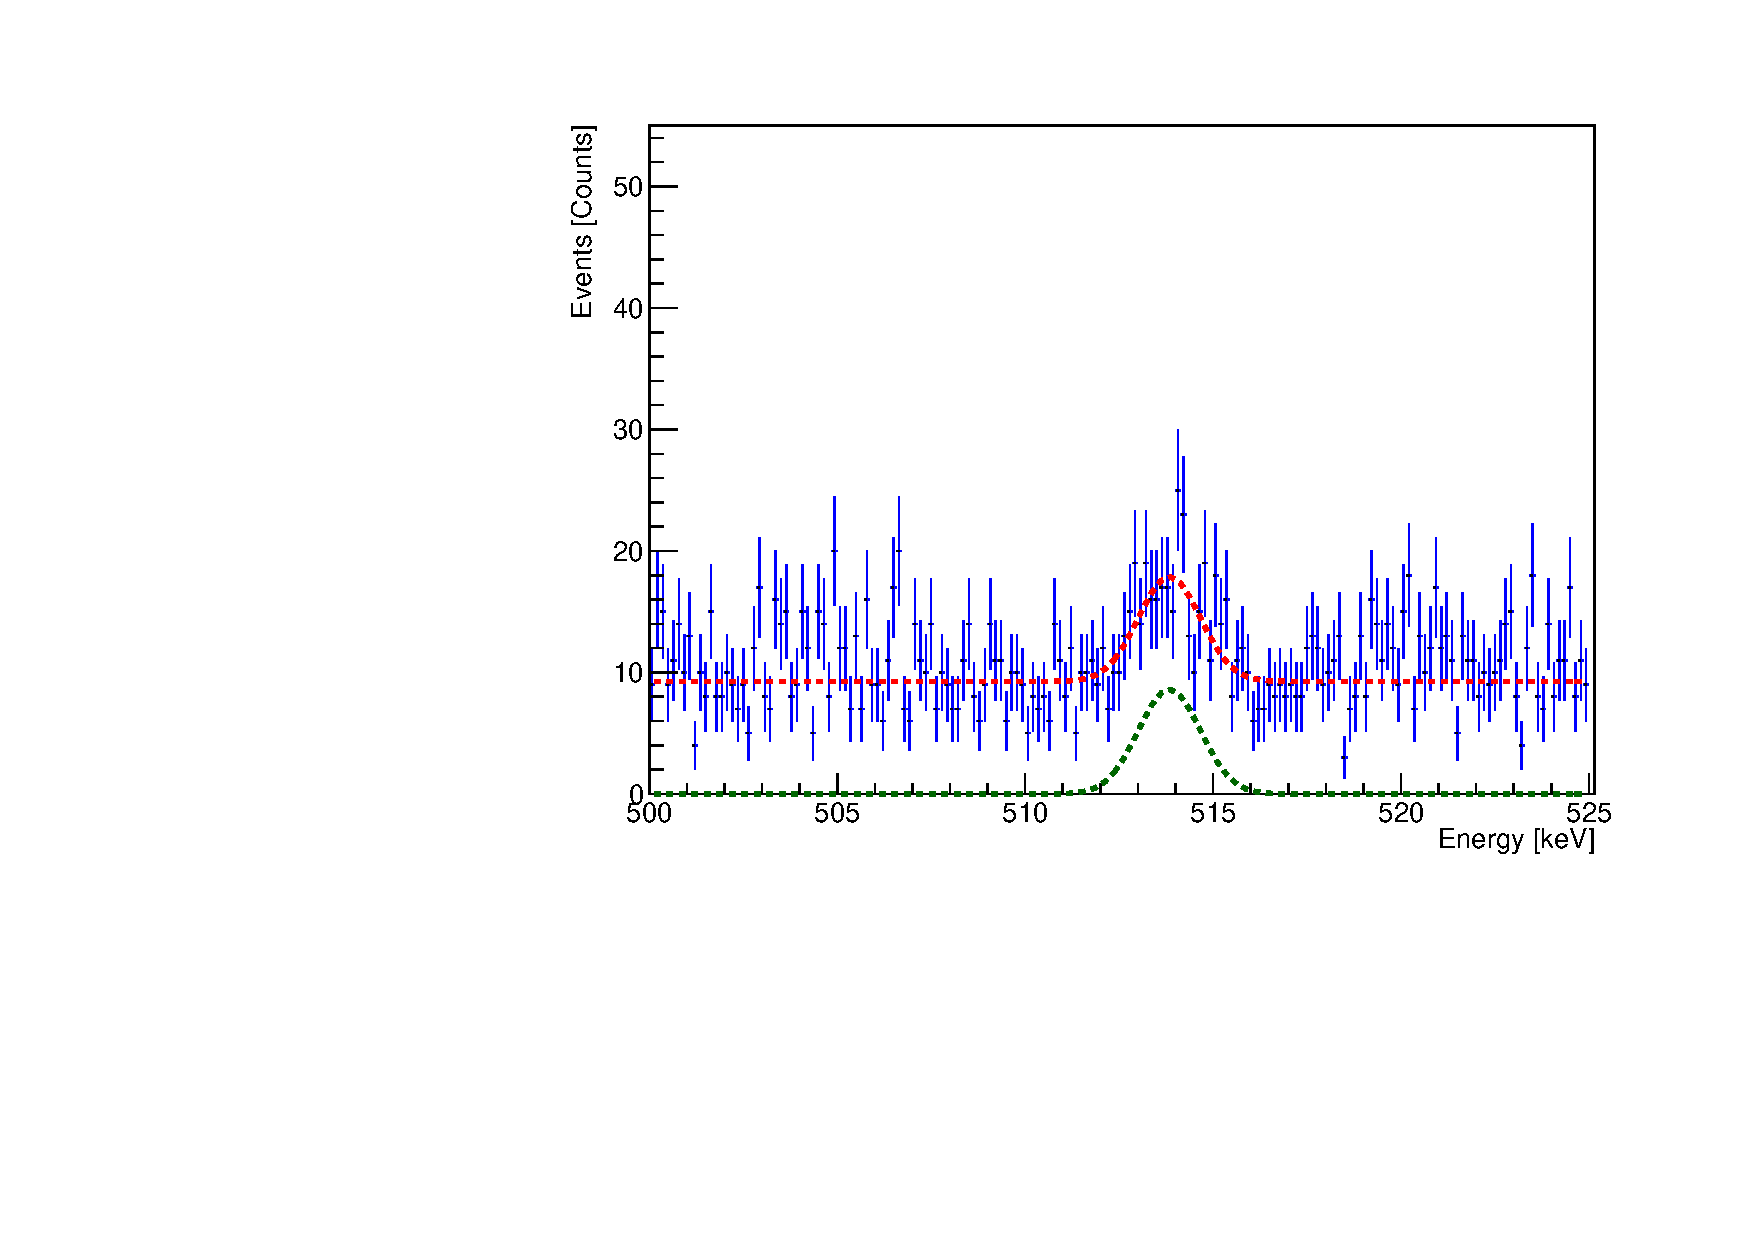
\includegraphics[width=75mm]{./Bilder/500525FitLArVetoBEGes.pdf}
		\caption{BEGes}
		\label{fig:FitLArVetoBEGes}
	\end{subfigure}%
	\begin{subfigure}{.5\textwidth}
		\centering
		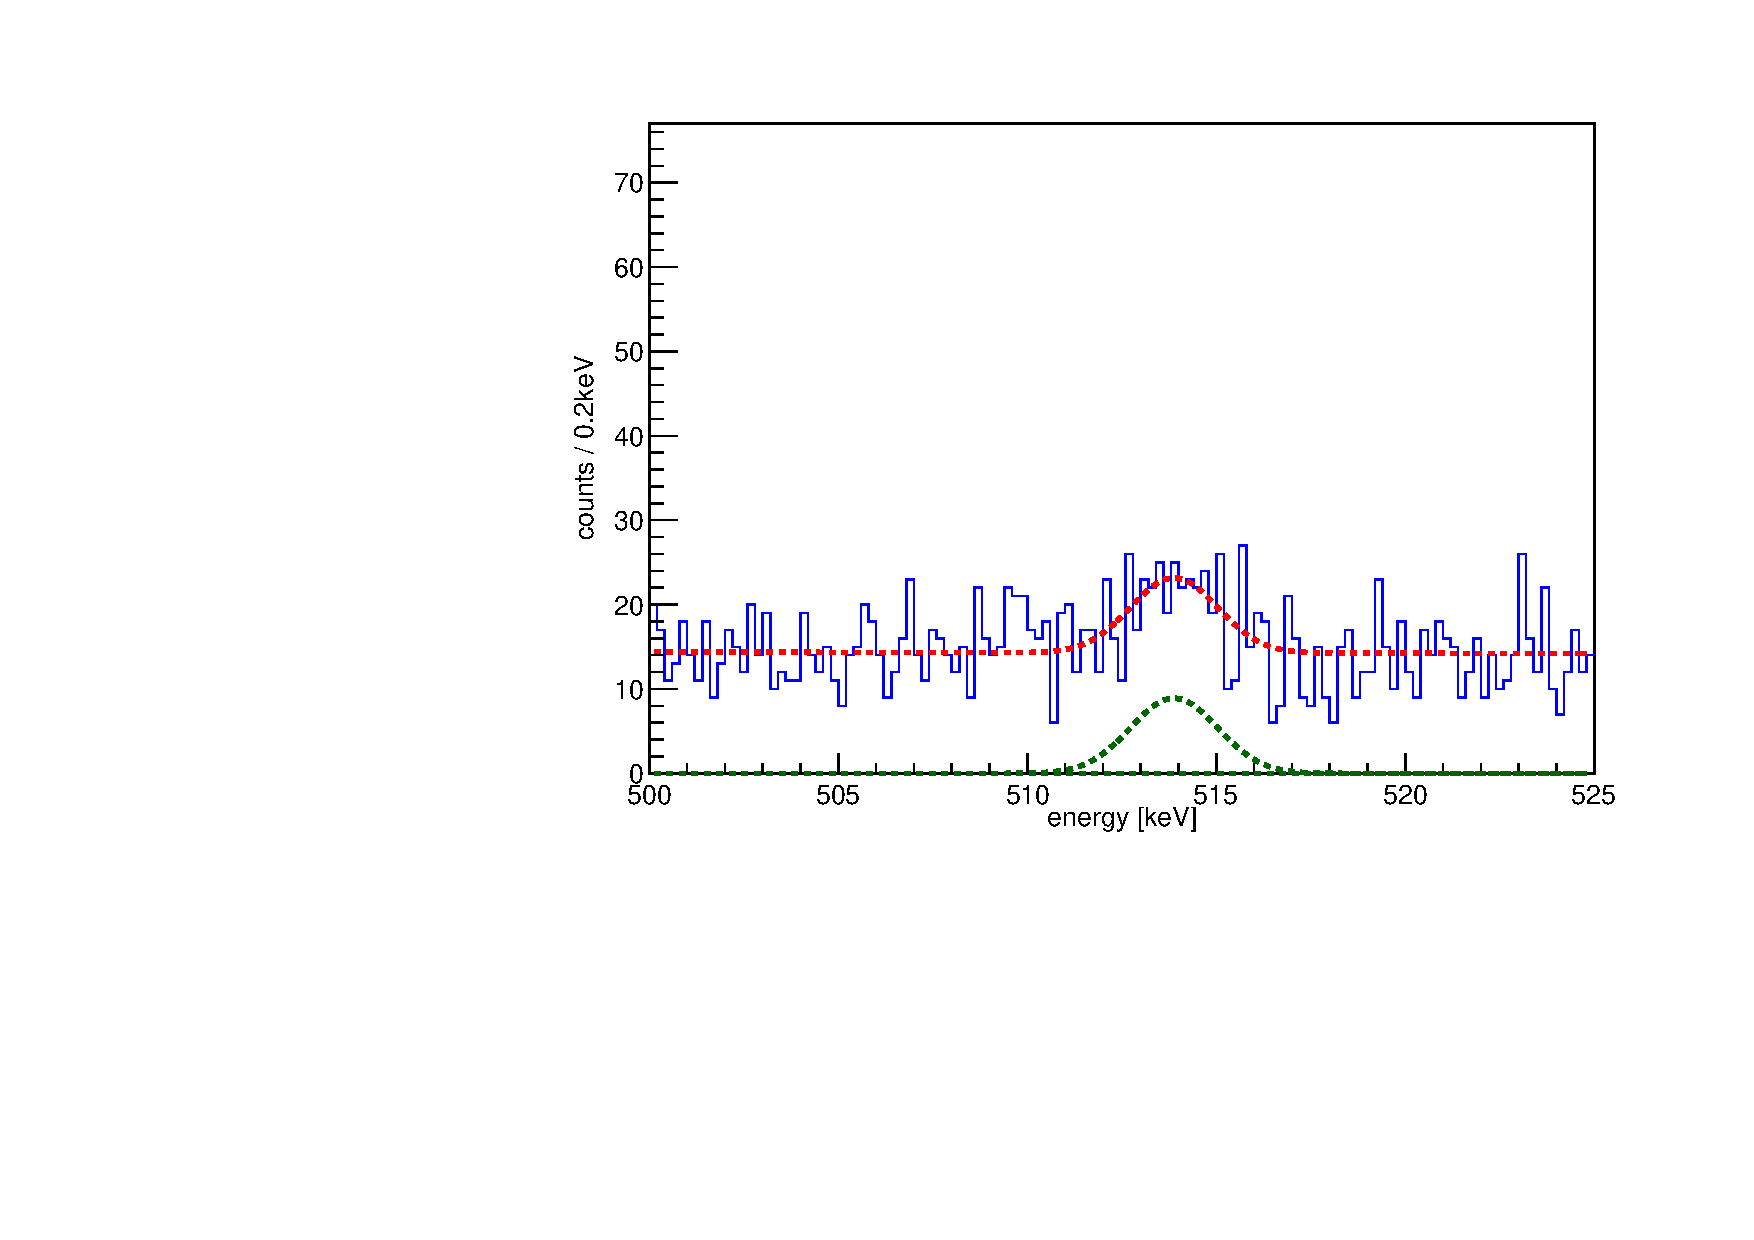
\includegraphics[width=75mm]{./Bilder/500525FitLArVetoCOAX.pdf}
		\caption{COAX}
		\label{fig:FitLArVetoCOAX}
	\end{subfigure}
	\caption{All events measured by the respective detectors  with the liquid argon veto applied in the range of 500keV to 525keV fitted with a fit function in the form seen in equation \ref{equ:FitFilters}.}
\end{figure}

\begin{figure}[t!]
	\centering
	\begin{tabular}{|l|r|r|r|r|}
		\hline
		Name	& Value [BEGes] \\ 
		\hline
		A  &	(17.844639 \(\pm\)	3.179471)&	(17.914476 \(\pm\)	2.683260)	&	(19.847330\(\pm\)	2.688415)&	(18.851511 \(\pm\)	2.696000)\\	
		\hline
		B  &	(513.838989 \(\pm\)	0.665171)&	(513.748535 \(\pm\)	0.179167)&	(513.849854 \(\pm\)	0.152052)&	(513.737183	\(\pm\) 0.167941)\\	
		\hline
		C  &	(0.828315 \(\pm\)	1.377836)	&	(0.940856 \(\pm\)	0.160788	)	&	(0.865958\(\pm\) 0.108436)&	(0.923679 \(\pm\)	0.149867)\\
		\hline
		D  &	(9.265341 \(\pm\)	1.032088)	&	(9.073170 \(\pm\)	0.233725	)	&	(9.307535\(\pm\)	0.236841)&	(9.076473 \(\pm\)	0.233940)\\
		\hline
		E  &	(18.142975 \(\pm\)	1.833031)	&	(-401772.843750 \(\pm\)	3.666062)	&	(-394189.968750\(\pm\)	45.660984)&	(-796827.062500 \(\pm\)	64.574379)\\
		\hline	
		F  &	(-26.647284 \(\pm\)	1.000000)	&	(-43.877174 \(\pm\)	1.414214	)	&	(-55.546192\(\pm\)	1.414214)&	(-55.546192 \(\pm\)	1.414214)\\
		\hline
	\end{tabular}
	\label{tab:FitParNoFilter}
	\captionof{table}[]{Fit parameters of fit function \ref{equ:FitNoFilters} applied on the spectra of the respective detectors.}
\end{figure}

Now that we have a number of the special \Kr events measured in the respective detectors.
But what we need for the determination of the activity is not the amount of measured events but actually the amount of \Kr decays in the whole liquid argon tank.
Luckily we can calculate the amount of actual events in the liquid argon tank by determining the detector efficiency of the two detector types.
This can be done by running a Monte Carlo simulation simulating a great amount of 514keV photon emissions in a cylindrical volume with a detector therein with the same design as used in GERDA.
From the amount of measured events in these simulated detectors and the absolute amount of simulated events one can then calculate the efficiency with which the detectors measure any \Kr events. 
How exactly this was implemented is the topic of the next chapter.
\\

\section{Monte Carlo Simulation}
\label{sec:MonteCarlo514}

As described above, we want to determine a conversion factor between the measured 514keV events and the decay density of \Kr necessary to create this signal.
Such a conversion factor can be determined with the help of a Monte Carlo simulation.
The tool used to perform this simulation is \mage (MAjorana-GErda), a GEANT4-based physics simulation software developed jointly by MAJORANA and GERDA \cite{boswell_mage_2010}.
Both experiments aim to measure the neutrinoless double beta decay using enriched Germanium detectors.
Because it is expected that the halflife of this decay is in the order of at least \(10^{25}\) years, a lot of effort is put into finding out how big the contribution of different isotopes to the background is.
\mage is therefor specialized to simulate radioactive decays and their corresponding measured events in Germanium detectors.
\\

The simulation used here consists of a cylindrical of 2.5m of height and 3m in diameter, in which the detector structure of the GERDA experiment is placed in the middle.
The resulting volume of the liquid argon is $V_{sim} = 17.65 \mathrm{m}^3$ .
Compared with the volume of 64 m\(^3\) of liquid argon used in the GERDA experiment this volume is much smaller.
But as we will see later, this volume is by far big enough for our purpose.
A total of N = 50.000.000 photons with an energy of 514keV are now simulated in of the volume in this cylinder that is not occupied by the detectors. 
As can be seen in figure \ref{fig:CrossSecAb}, the density of the decays over the entire volume of the cylinder is relatively constant.
\\

\begin{figure}[t!]
	\centering
	\begin{subfigure}{.5\textwidth}
		\centering
		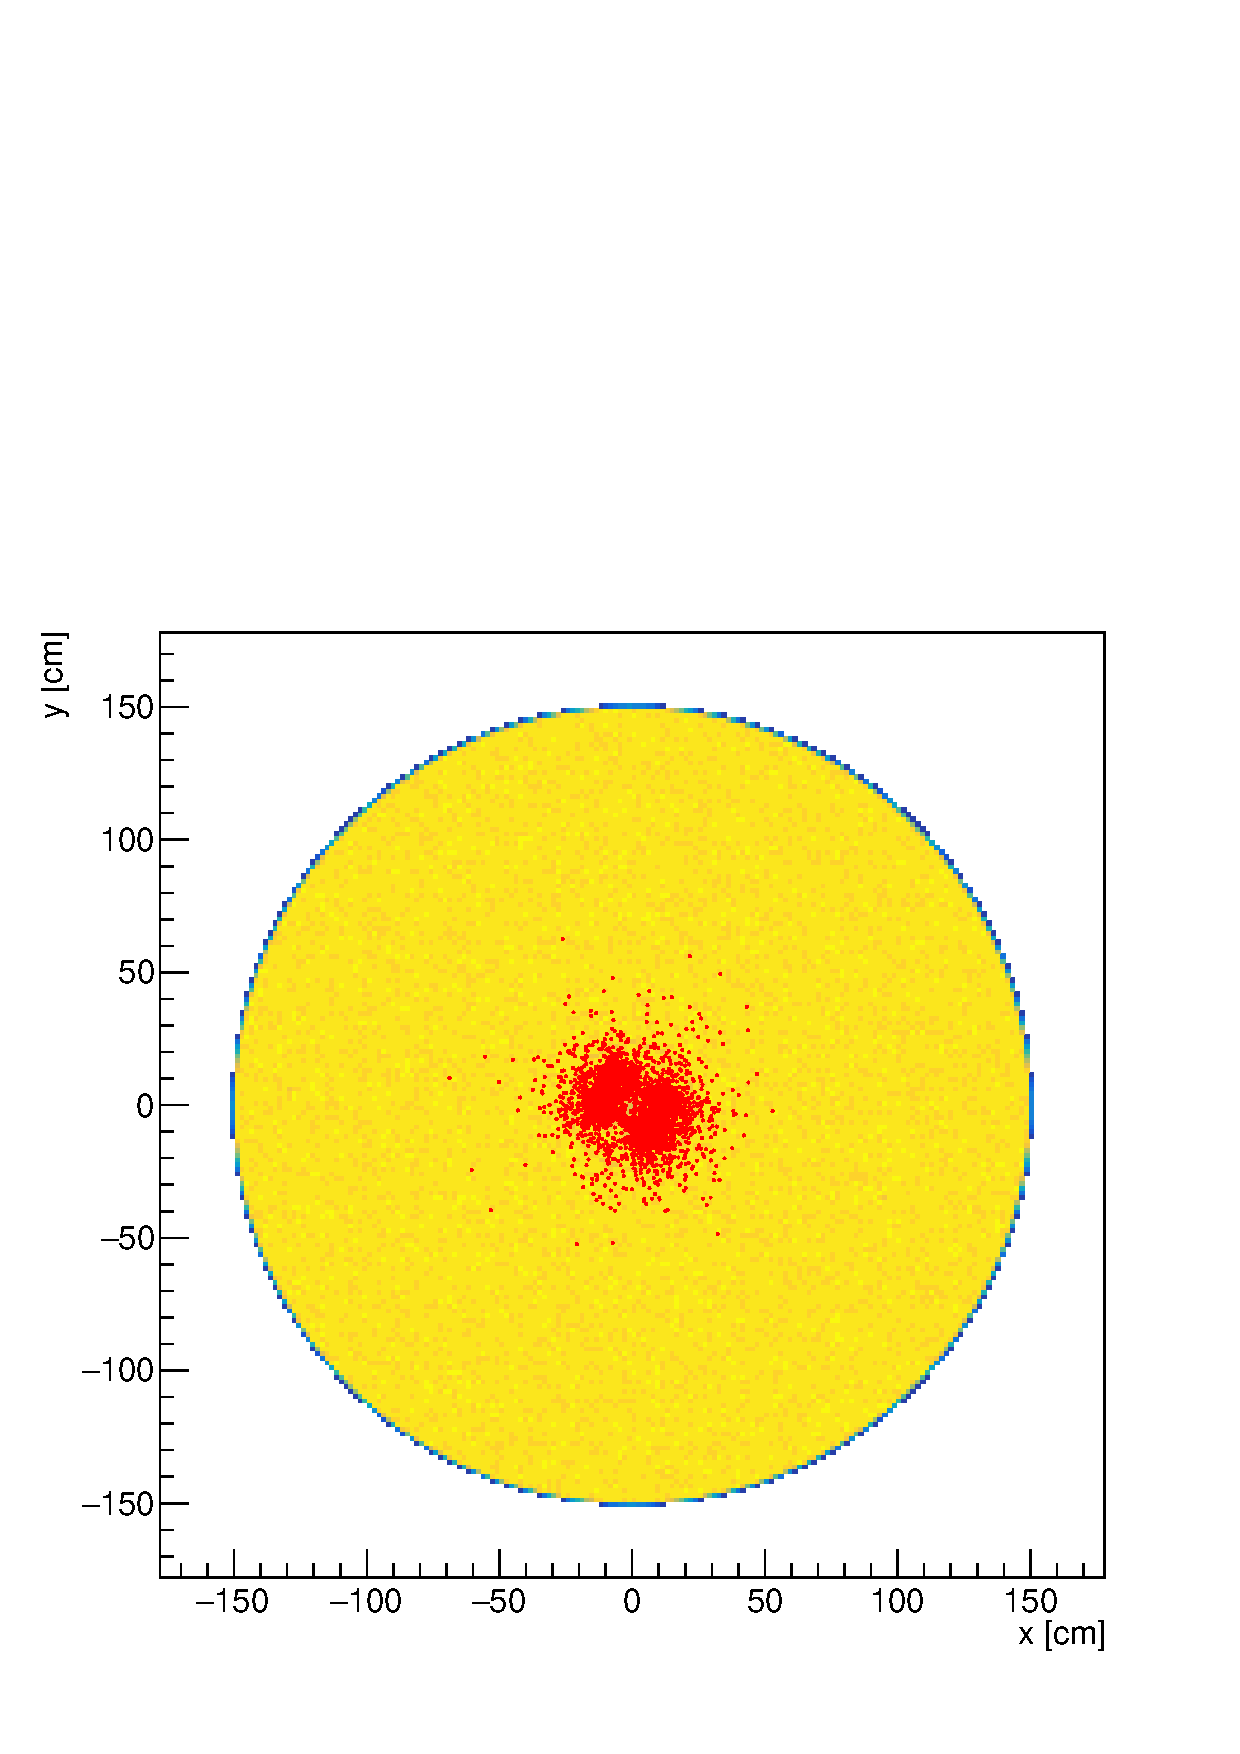
\includegraphics[height=75mm]{./Bilder/MC-Querschnitt-BEGes.pdf}
		\caption{Cross section from above}
		\label{fig:CrossSecAb}
	\end{subfigure}%
	\begin{subfigure}{.5\textwidth}
		\centering
		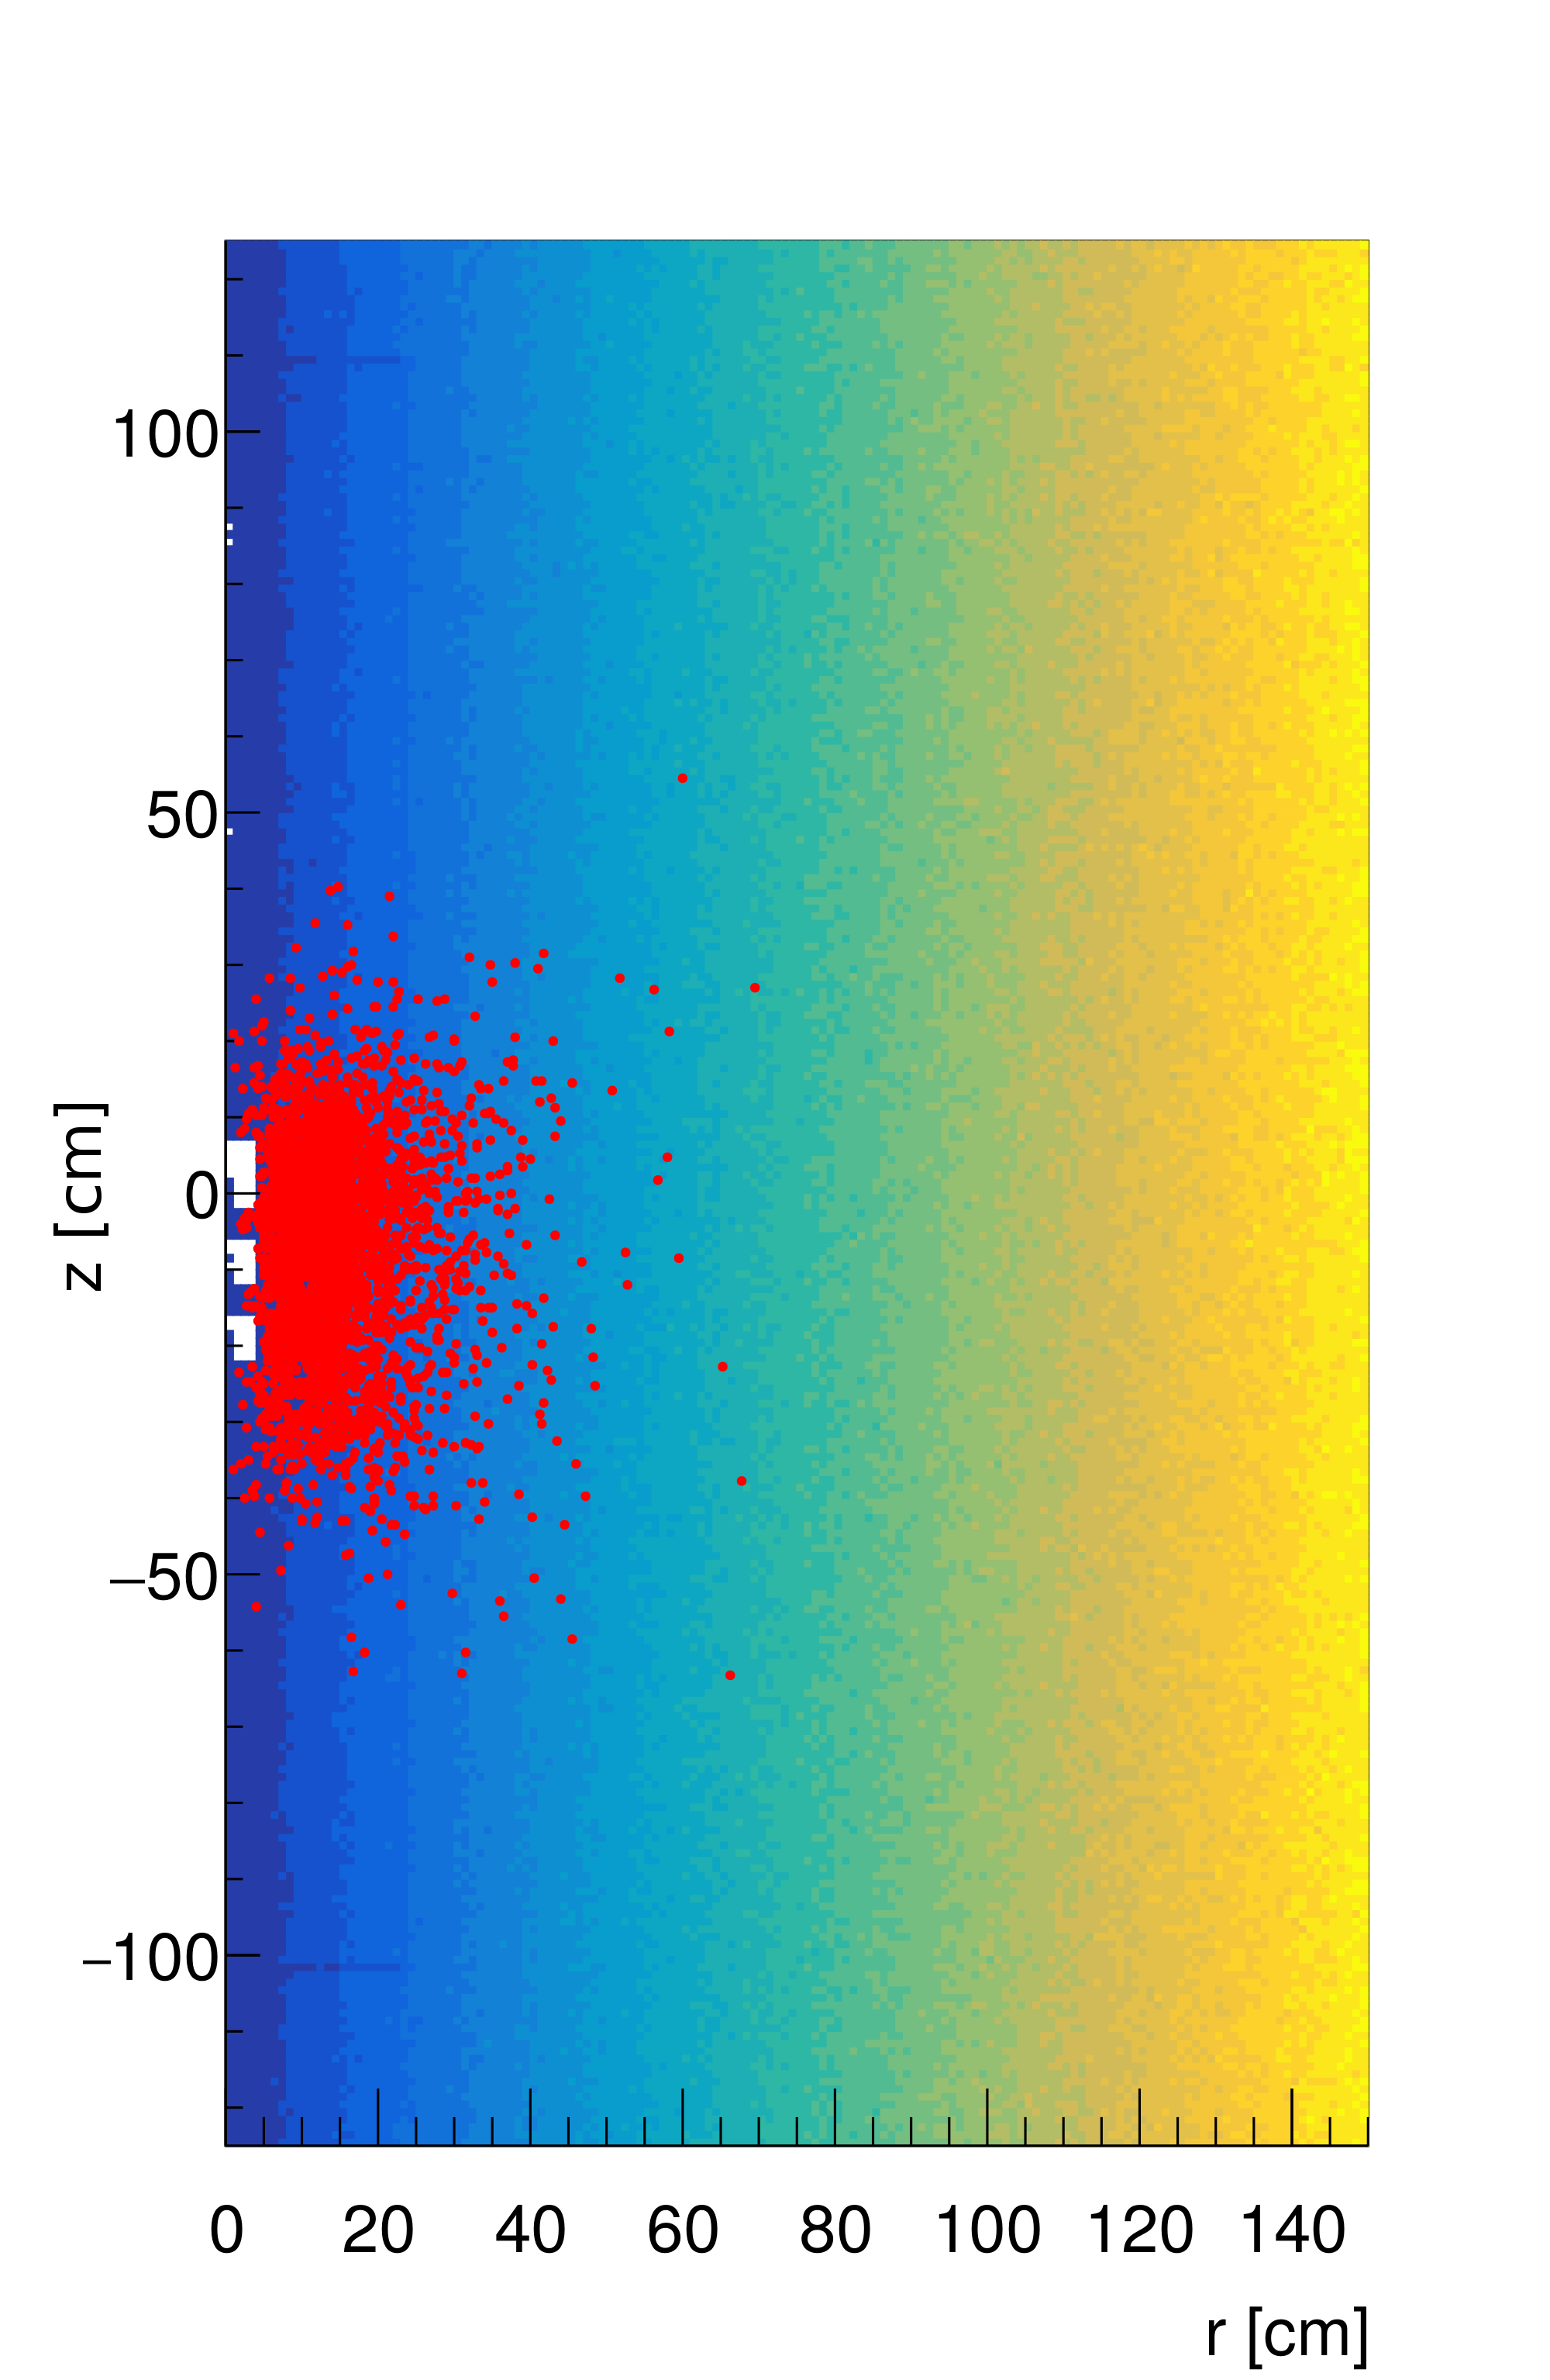
\includegraphics[height=75mm]{./Bilder/MC-Radius-BEGes.png}
		\caption{Radial cross section}
		\label{fig:CrossSecRa}
	\end{subfigure}
    \\
	\vspace{0.5cm}
    \caption{Cross section from above and a radial cross section showing the density of simulated decays in the cylindrical volume. The red points indicate all events that were measured by the BEGe detectors.}
\vspace{0.5cm}
\end{figure}
\\

From these 50 million simulated decays only about 90 thousand were actually detected by any of the detectors, only 30.465 of them crated a signal in one of the BEGe and 24.902 in the COAX under the condition that one already uses an anti-coincedence filter.
The spatial distribution of all measured events in the respective detectors can be seen as red dots in Figure \ref{fig:CrossSecAb} and \ref{fig:CrossSecRa} for the BEGe detectors and Figure blah and blah for the COAX detectors, depending on the detector type.
From their position one can see that in both detector types the overwhelming majority of the detected events were positioned close to the detectors themselves.
Already at a distance of about 60cm from the detectors the majority of all decays were no longer measured.
This means that the amount of measured events should not change when one enlarges the volume of the tank, provided that the density of decays stays constant.
But that would also mean that the detector efficiency $\epsilon$ would have a reciprocal proportionality to the simulated volume.
Therefore, we expect the ratio $\frac{1}{\epsilon V_{sim}}$ to be invariant with change of volume, provided that the volume is large enough.   
This is the reason why we are able to use a smaller volume of liquid argon in the Monte Carlo simulation than was actually used in the experiment.
At the same time, this ratio is also a conversion factor between the amount of measured 514keV photons and the density of \Kr necessary to create the measured peak, which is exactly what we want to determine with this simulation.
\\

The spectrum of all the events detected in BEGe detectors is shown in figure \ref{fig:PhasenraumMC514}.
From it one can be seen that only a small amount of all measured events are direct signals from a rare \Kr decay. 
The great majority of photons measured were scattered before they arrived in the detector and therefor have a lower energy.
Among other things, the Compton edge of the photons at about 343 keV can be seen.
But to calculate the detector efficiency, only the measured events at the 514keV peak have to be used.
In the case of the BEGe detectors this peak contains a total of \(\Delta\mathrm{N} = 4511\pm67\) events while the COAX peak contains  \(\Delta\mathrm{N} = 3706\pm60\) .
With a total of 50 million initial decays, this results in a efficiency of 
\begin{equation*}
\epsilon_{\gamma\mathrm{,BEGe}} = \frac{\Delta\mathrm{N_{BEGe}}}{\mathrm{N}} = (9.02\pm0.13) \times 10^{-5}  \frac{\mathrm{event}}{\mathrm{decay(rare)}}
\end{equation*}
\begin{equation*}
\epsilon_{\gamma\mathrm{,COAX}} = \frac{\Delta\mathrm{N_{COAX}}}{\mathrm{N}} = (7.412\pm0.12) \times 10^{-5}  \frac{\mathrm{event}}{\mathrm{decay(rare)}}
\end{equation*}
for the volume of the simulated cylinder.
\\

This means that if a 514keV photon is emitted at any location in the liquid argon container, it has a probability \(\epsilon_{\gamma,\mathrm{,BEGe}}\) of being measured by one of the BEGe detectors.
On the other hand, it can also be said, that for every measured 514keV photon in one of the BEGe detectors an amount of about $\frac{1}{\epsilon_\gamma} = 10515 \frac{\mathrm{decay(rare)}}{\mathrm{event}}$ \nuc{Rb}{85m} relaxations must occur.
In other words, the value $\frac{1}{\epsilon_\gamma}$ is a factor from the measured entries to the actual amount of \nuc{Rb}{85m} relaxations.
If you divide this factor by the simulated volume you get the conversion factor you want to determine with this simulation.

\begin{equation*}
\frac{1}{\epsilon_{\gamma\mathrm{,BEGe}} V_{sim}} = (5.955\pm0.086) \times 10^{-1} \frac{\mathrm{photon}}{\mathrm{event} \times l}
\end{equation*}
\begin{equation*}
\frac{1}{\epsilon_{\gamma\mathrm{,COAX}} V_{sim}} = (5.955\pm0.086) \times 10^{-1} \frac{\mathrm{photon}}{\mathrm{event} \times l}
\end{equation*}

As mentioned above these values are invariant with change of volume which is why we can also apply it to our real liquid argon tank volume. 
\\

\begin{figure}[t!]
	\centering
	\ifmakefigures%
	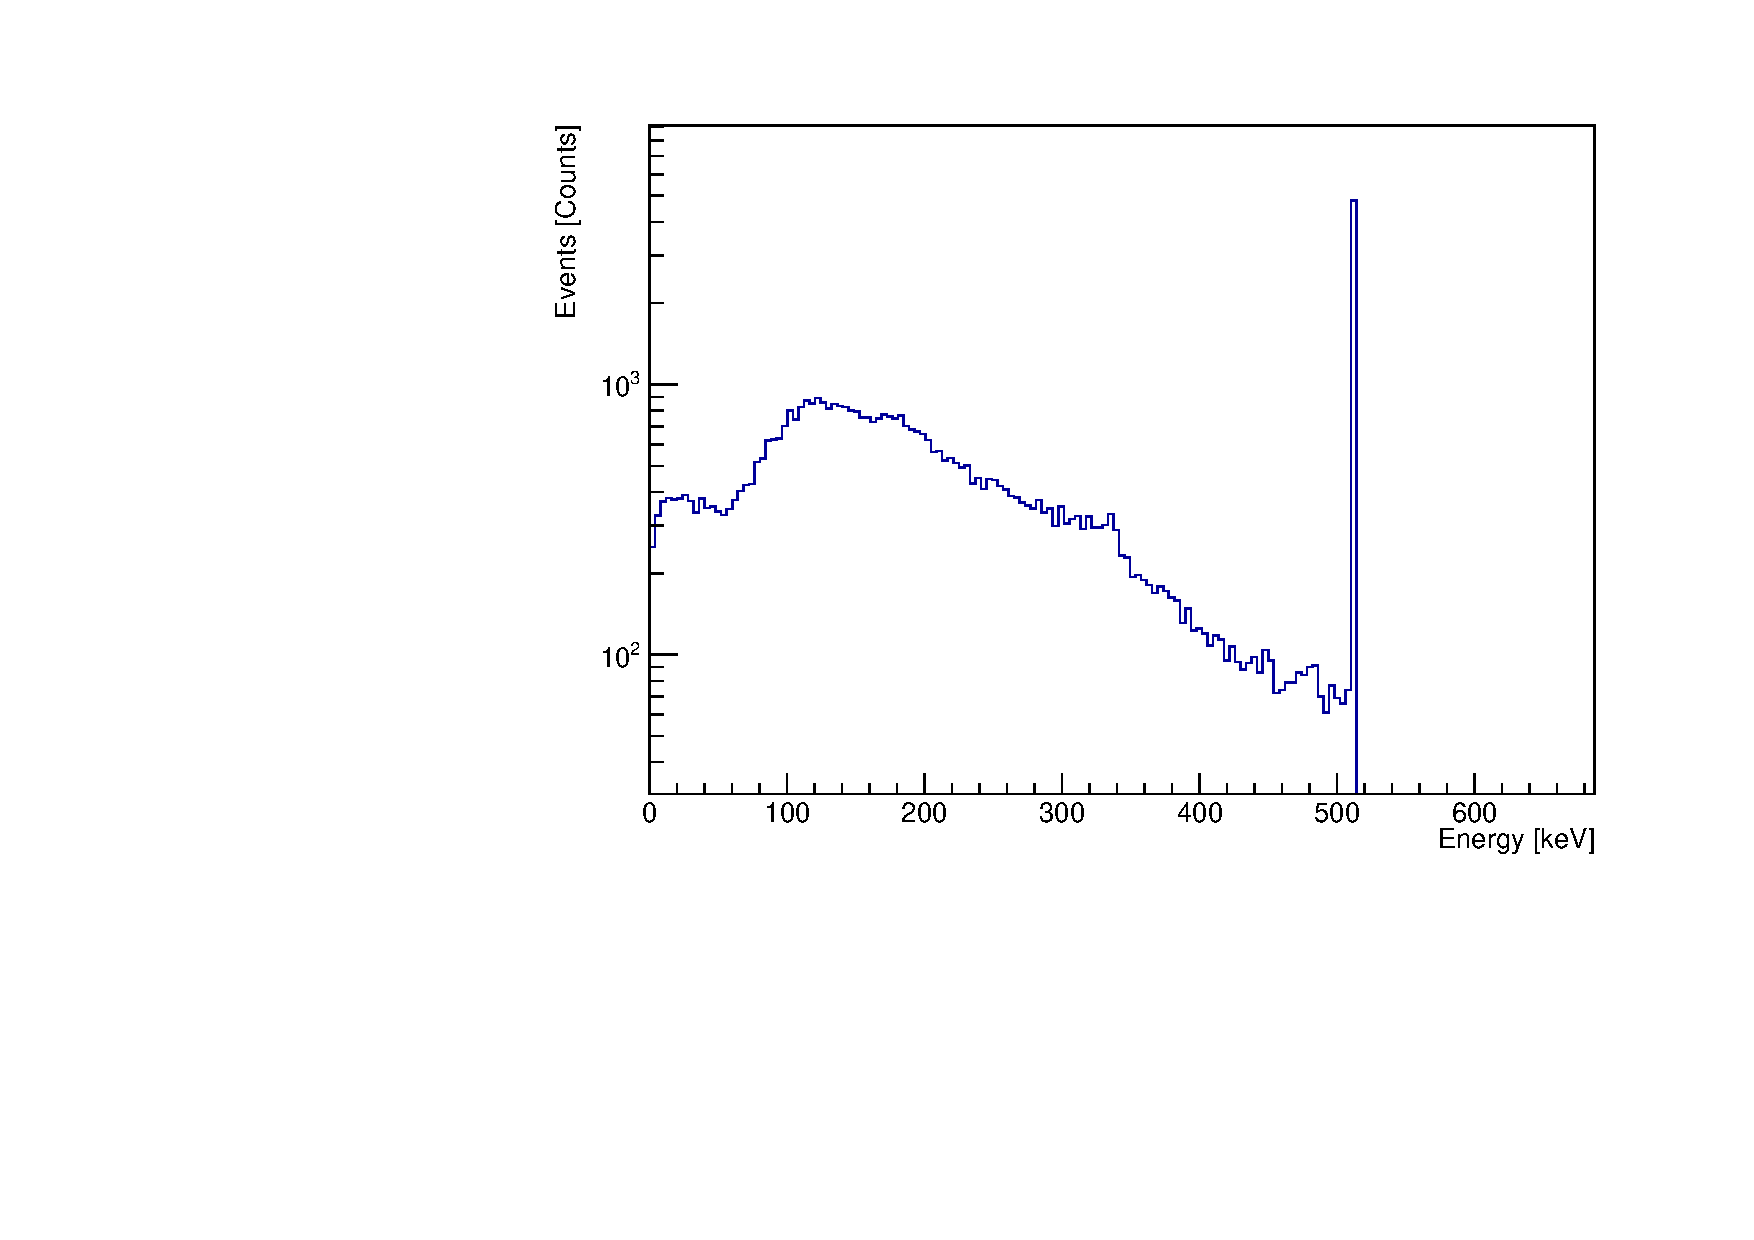
\includegraphics[width=100mm]{./Bilder/MC-514-Phasenraum.pdf}
	\fi%
	\caption{
    Spectrum of the measured rare \Kr events in all of the BEGe detectors of the Monte Carlo simulation.
	}
	\label{fig:PhasenraumMC514}
\end{figure}

Now that the conversion factors of the two types of detectors are determined we can calculate the density of all \Kr decays by applying formula \ref{equ:density}

\begin{equation}
\rho_{dec} = \frac{\mathrm{N}}{p}\times\frac{1}{\epsilon_\gamma V_{sim}}
\label{equ:density}
\end{equation}

where p = 0.434$\%$ is the probability of a \Kr to decay into the 514keV energetically raised \nuc{Rb}{85m}.
For an amount of 27.24\(\pm\)3.87 events to be measured in the BEGe detectors, it can be concluded that a density for the \Kr decay of, whereas for the COAX detectors we get a value of . 
\\


\section{Calculating the Activity}
\label{sec:CalcActiv}

All we need now to calculate the mean activity of \Kr in \PII is the measuring time of all detectors.
But this is not as easy as it seems.
Firstly we have the problem that not all detectors were measuring over the curse of \PII and that there were time intervals in which no measurement was recorded at all.
This can easily be solved by looking at the effective measuring time of each detector individually.
The effective measuring time of a detector can easily be determined by looking at how many test pule signals have been recorded by it. 
Since the test pulse signals have been set to a frequency of 0.05Hz over the entire \PII, an effective measurement time can be achieved by determining the number of detected test pulse signals and then multiply it by 20 seconds.
The individual measuring times are therefor given by
\begin{equation*}
    t_\mathrm{i} = \mathrm{N}_{TP}(\mathrm{i}) \times 20\mathrm{s}
\end{equation*}
where i is the index of the respective input channel of each BEGe detector.
\\

The second problem arises from the fact that we calculated the decay density with the assumption that we could merge all detectors of the same kind into a single detector.
But now that we want to look at the measurement time of each individual detector, this assumption does not hold true.
There are now two different workarounds we could take.
\\

In the first method we would rerun our Monte Carlo simulation, this time considering the amount of time each detector was actually measuring.
This would be very inefficient.
\\

The second method works around the merging problem by calculating an average measurement time for all detectors.
With this you could then calculate with the detector block as if all detectors of one kind were such a single detector.
This is very elegant solution because no new computation of a simulation is necessary.
\\

For this average measuring time one has to consider the fact that we also have to apply a weigh on every individual measuring time.
This arises from the fact that every BEGe detector has an individual mass.
As we know, the detector efficiency of a single detector is directly dependent on its mass.
If we want to combine all single detectors into one large detector, we have to consider that heavier detectors contribute more to the measured decay rate than lighter detectors.
It is therefore necessary to weight the measuring time of each detector with its individual mass.
Coincidentally, the multiplication of the individual measuring time of a detector with its mass is also the exposure this  single detector.
This means that to calculate the mean measuring time, we just have to divide the combined exposure of all detectors of the same kind by their combined mass.
\\

No matter what approach you take, you can now determine the mean measuring times using equation \ref{meanmeauringtime}.

\begin{equation*}
    \bar{t} = \frac{\sum_\mathrm{i} t_\mathrm{i} \times m_\mathrm{i}}{\sum_\mathrm{i} m_\mathrm{i}} = 1.592
\label{meanmeauringtime}
\end{equation*}

From this, an average measurement time for the BEGes of  and for the COAX of can be calculated.
With these mean measuring times we can now finally calculate the mean specific activity $\bar{a}$ of \Kr over the curse of all of \PII by applying
\begin{equation*}
    \bar{a} = \frac{\rho_{dec} }{\bar{t}} = \frac{\mathrm{N}}{p}\times\frac{1}{\epsilon_\gamma V_{sim}}\times\frac{1}{\bar{t}}
\end{equation*}


With the line count rate analysis we are now finally able to determine an activity of $\bar{a}_{\mathrm{1,BEGe}} = (5.46\pm0.827)\times10^{-4}	\frac{\unit{Bq}}{\unit{l}}$ in the BEGes and a specific activity of $\bar{a}_{\mathrm{1,COAX}} = (4.70\pm0.887)\times10^{-4}	\frac{\unit{Bq}}{\unit{l}}$ in the COAX.
These two values differ only inside their range of uncertainty which is why these results are of good quality.
Of these two value we can now also calculate a mean specific activity $\bar{a}_{1} = (5.08\pm0.857)\times10^{-4}\frac{\unit{Bq}}{\unit{l}}$.
\\

We can now make some comparisons of this value with the WARP and the Darkside experiments.
In the case of the WARP experiment a specific activity of $(160\pm130)\frac{\unit{mBq}}{\unit{l}}$ \label{} was measured for the \Kr.
On the other hand, an specific activity of $(2.8577 \pm 0.18122) \frac{\unit{mBq}}{\unit{l}}$ was measured in the Darkside experiment.
Our determined value of $(0.508\pm0.085)\frac{\unit{mBq}}{\unit{l}}$ is about one order of magnitude smaller than the specific activity in the Darkside and whole three orders of magnitude smaller than the WARP experiment.
From these comparisons we can see that our results seem to verify the first approximations mentioned in the introduction predicting that the \Kr activity seems to be much smaller than in other experiments using liquid argon.
\\

What we can also do now is take the specific activities of the other two experiments and determine how many counts we would have measured if the \Kr had their specific activity.
As simplification we restrict ourselves here to the theoretical values that could be measured in the BEGe detectors. 
How many counts the corresponds activity would induce in the BEGe detectors we can determine with the help of formula \ref{equ:correspondingEvents}.
\begin{equation}
\mathrm{N} = \bar{a} \times p \times \epsilon_\gamma V_{sim} \times \bar{t}
\label{equ:correspondingEvents}
\end{equation}
With the activity and the values determined from the analysis above we can calculate a corresponding amount of about 76152 events for the WARP experiment and 1360 in the Darkside experiment.
In the case of the WARP experiment one could expect with such a high activity that the count rate is also much higher than the 183 events determined from the actual measurement.
Again for the Darkside experiment we calculate a amount of counts about one order of magnitude higher than the here measured events.
From these comparisons we can see that for a much higher specific activity of \Kr to have actually been present a much bigger amount of events should have been counted.
As a graphical representation, the peaks that one would have been able to be seen in the measured spectrum are displayed in figure \ref{fig:WARP} and \ref{fig:Darkside}.
In both diagrams the actually measured spectra are also displayed, even if they are not recognizable as in the case of the WARP peak.
\\

\begin{figure}[t!]
	\centering
	\begin{subfigure}{.5\textwidth}
		\centering
		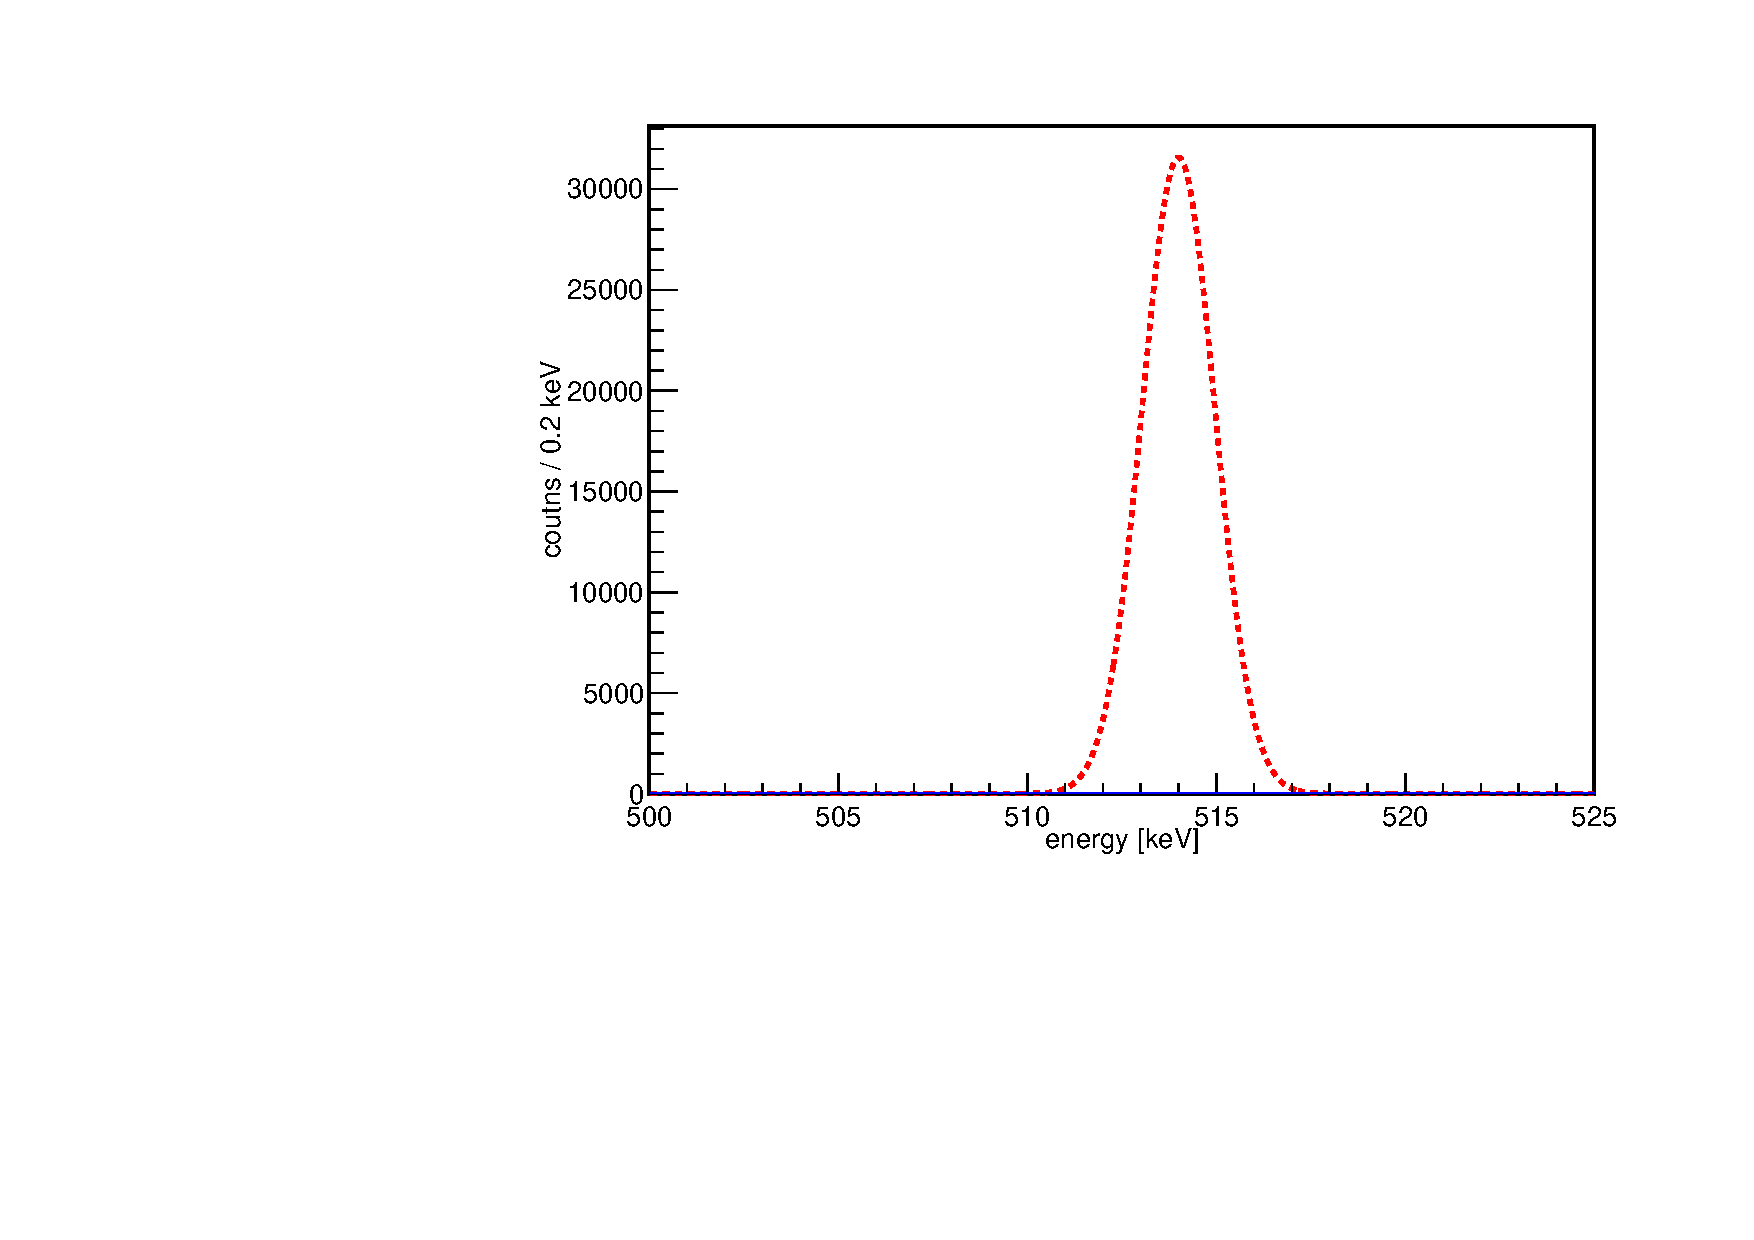
\includegraphics[width=75mm]{./Bilder/WARP.pdf}
		\caption{Cross section from above}
		\label{fig:WARP}
	\end{subfigure}%
	\begin{subfigure}{.5\textwidth}
		\centering
		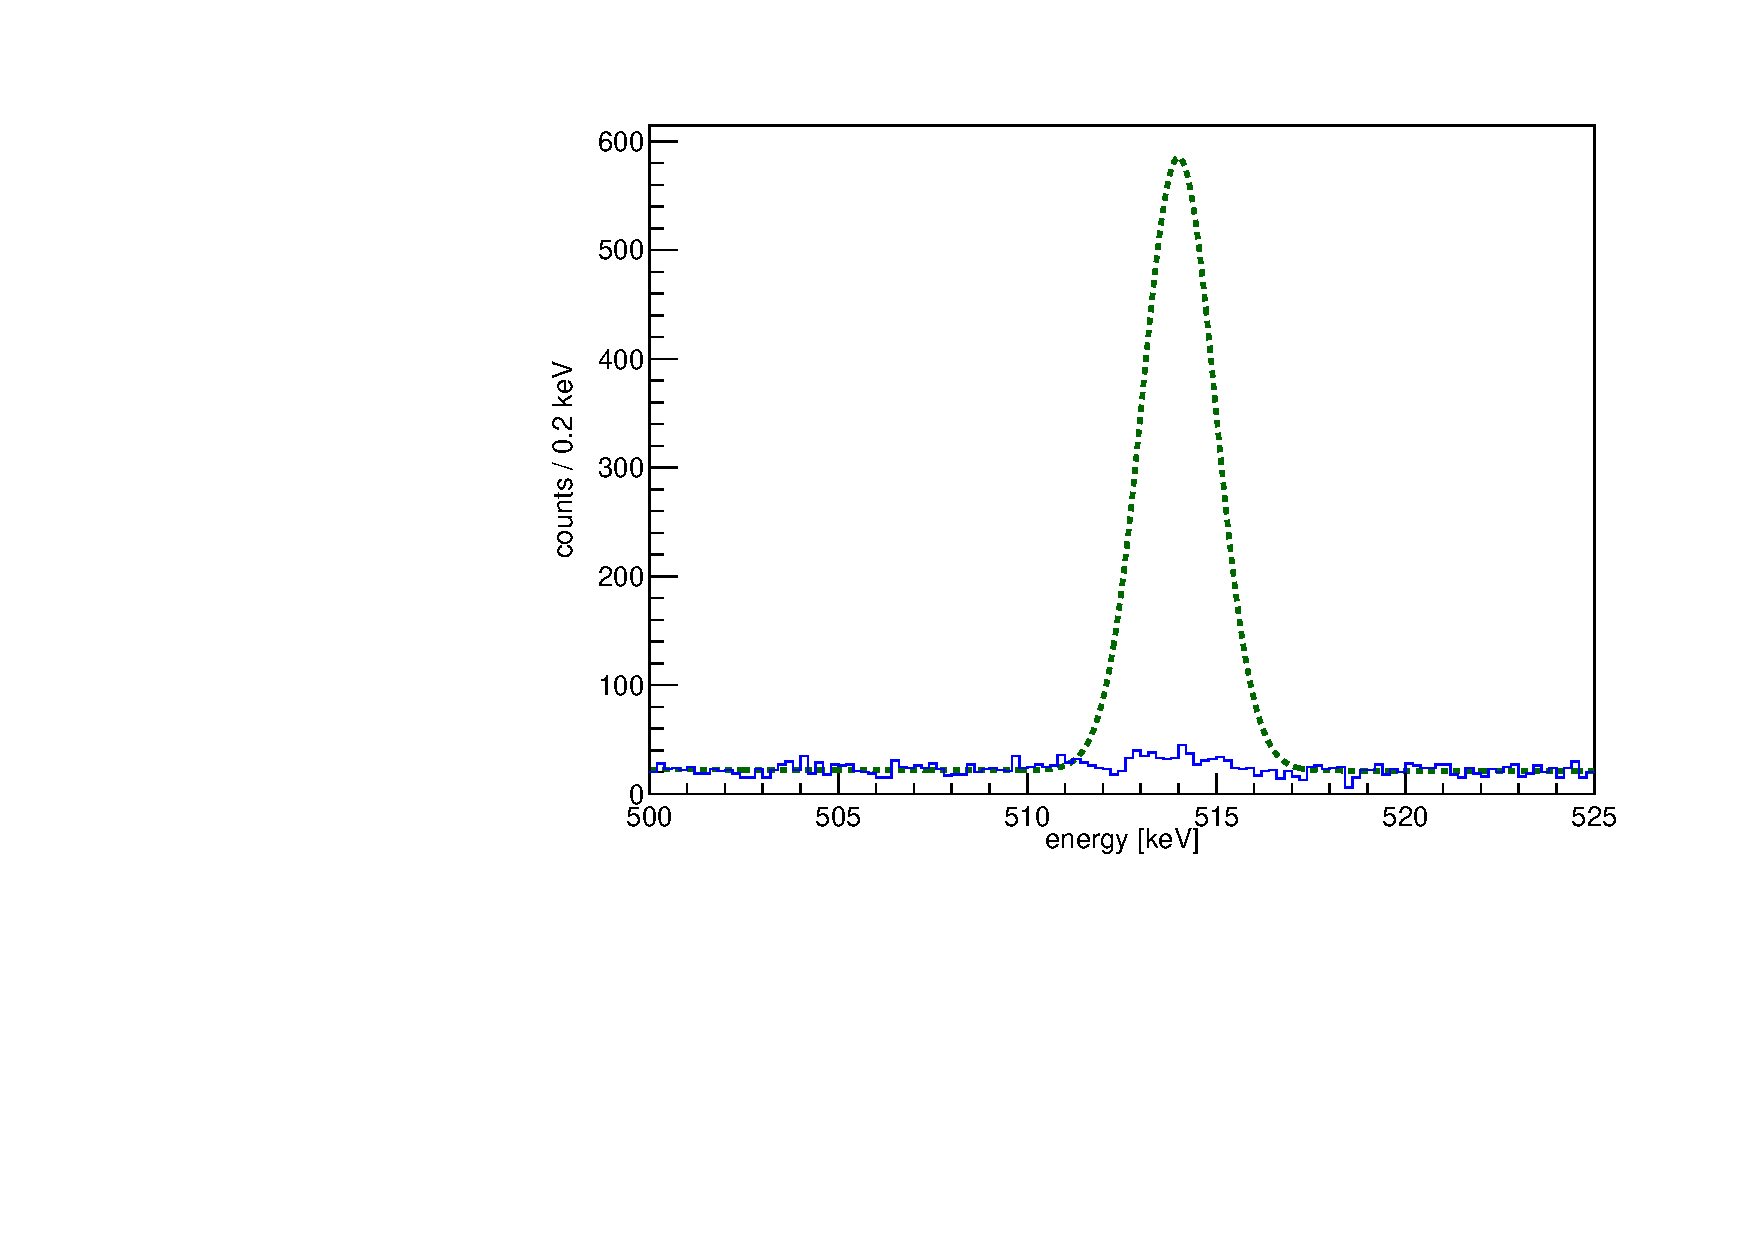
\includegraphics[width=75mm]{./Bilder/Darkside.pdf}
		\caption{Radial cross section}
		\label{fig:Darkside}
	\end{subfigure}
    \\
	\vspace{0.5cm}
    \caption{}
\vspace{0.5cm}
\end{figure}
\\

Now that we have determined a concrete value for the specific activity of \Kr we now come to our second attempt to measure the specific activity as described in the next chapter.
\\  




%	4.70E-04	8,87E-05	Bq/l


% calculate Amplitude of Gauss peak at 514keV and use factor from Monte Carlo Simulation to estimate

% look at phase diagram at range of 500 to 525 keV, use different filters and fit remaining data with Gaussian function
% -> get amplitude
% make a Monte Carlo simulation to estimate actual Kr85 activity in LAr from measured activity in detectors
% -> with amplitude and factors from MC-Simulation one can calculate the specific activity

\chapter{Activity from the Decrease in Rate}
\label{sec:SAfromDecrease}

As described in the beginning of section \ref{sec:AotKr}, the line count analysis method of the rare \Kr decay was expected to be relatively precise.
By following this procedure we were able to determine the activity down to the order of 10$^{-4} \frac{\mathrm{Bq}}{\mathrm{l}}$ with reasonable uncertainty.
We will now concentrate on implementing and discussing the second approach of determining the specific activity by using the change of event rate over time.
Because this method does not rely on any of the values used in the line count rate analysis this approach is truly completely independent of the other method.
Ideally, a positive result from this method would confirm the specific activity determined in the previous chapter. 
\\

But as it was also stated above, the second method is expected to be relatively imprecise.  
This estimation came from the fact that this method relies on a great approximation.
For this method to be applied it is necessary to expect that in the time interval of all of \PII only the intensity of the \Kr isotope has a non negligible change in its intensity.
The idea behind this comes from the fact that \Kr has the lowest half life \(T = 10.739\unit{y}\) of all the other residual radioactive isotopes in the liquid argon.
In comparison, other radioactive isotopes that are of interest here are \nuc{Ar}{42} with a half-life of 32.9 y \cite{chen_nuclear_2016}, \nuc{Ar}{39} with 269 y \cite{singh_nuclear_2006} and \nuc{Po}{210} with 138d \cite{kondev_nuclear_2008}. 
\\

\nuc{Po}{210} has a much lower half life than \Kr but the energy of the escaping alpha particle much higher than the mean beta energy of all of the isotopes above.
This is important, because over the course of this chapter we will at some point begin to only consider those events in our analysis that deposited an energy between 200 and 400 keV.   
This means even though \nuc{Po}{210} has a much lower half life it would not create much of a change in event rate due to its very low probably to release an alpha particle in this energy range.
\\

On the other hand, the two different types of argon isotopes have both a mean beta energy close to \Kr's 251.59 keV.
Their change in event rate should therefor be measurable by our approach.
The change in activity of \nuc{Ar}{39} can be neglected because its half life way to big.
\nuc{Ar}{42} on the other hand has a half life that is in the same order of magnitude as \Kr.
But its specific activity has already been determined to be about $148\mui Bq/l$ \cite{becerici_schmidt_results_2014} which is about factor 3.5 smaller than the expected \Kr specific activity.
Whether or not we have to consider the influence of this isotope will be discussed later in this theses.
For now we will apply the simplification that its change will be small compared to \Kr.
\\

All other radioactive isotopes that are residual in the liquid argon have either a much longer half life than \nuc{Ar}{42}, their mean beta energy is much higher than 400keV or their specific activity is too small too small to measure any kind of change over time.
It is therefor approximated that all change in intensity should only originate from the \Kr decay.
But even if the activity determined by this method is not expected to have a much of a value for us, it can still be used as a crosscheck for the other activity determined above.
\\

We have now shown that this approach can be applied here and that it actually serves a purpose.
Now it has to be discussed how exactly the specific activity can be determined by changing the intensity.
To measure the change in rate every measured event will have to be drawn over time and through it an exponential fit applied.
The amplitude of the resulting exponential function represents an event rate with which events in the investigated energy range occur.
\\

To calculate the specific activity of \Kr with this value one again has to use a Monte Carlo simulation to calculate a fitting conversion factor. 
We cannot use the same simulation from the first method because in this case we actually have to simulate \Kr events, not only the emission of 514keV photons as it was done in the prior chapter.
That is why another Monte Carlo simulation has to be carried out.
With it a new conversion factor can be determined to calculate the \Kr decay density necessary to create the measured event activity.
\\

Finally the specific activity can be calculated from these two values.
It is important to note that this approach determines the specific activity of \Kr at the start of \PII while the first method calculates the mean specific activity over all of \PII.
To compare those two results, in the end a mean specific activity of the second method has to be determined.
The following sections will focus on the concrete implementation of this method and the values determined by them.
\\

\section{Event Rate}
\label{sec:EventAct}

\begin{figure}[t!]
	\centering
	\begin{subfigure}{.5\textwidth}
		\centering
		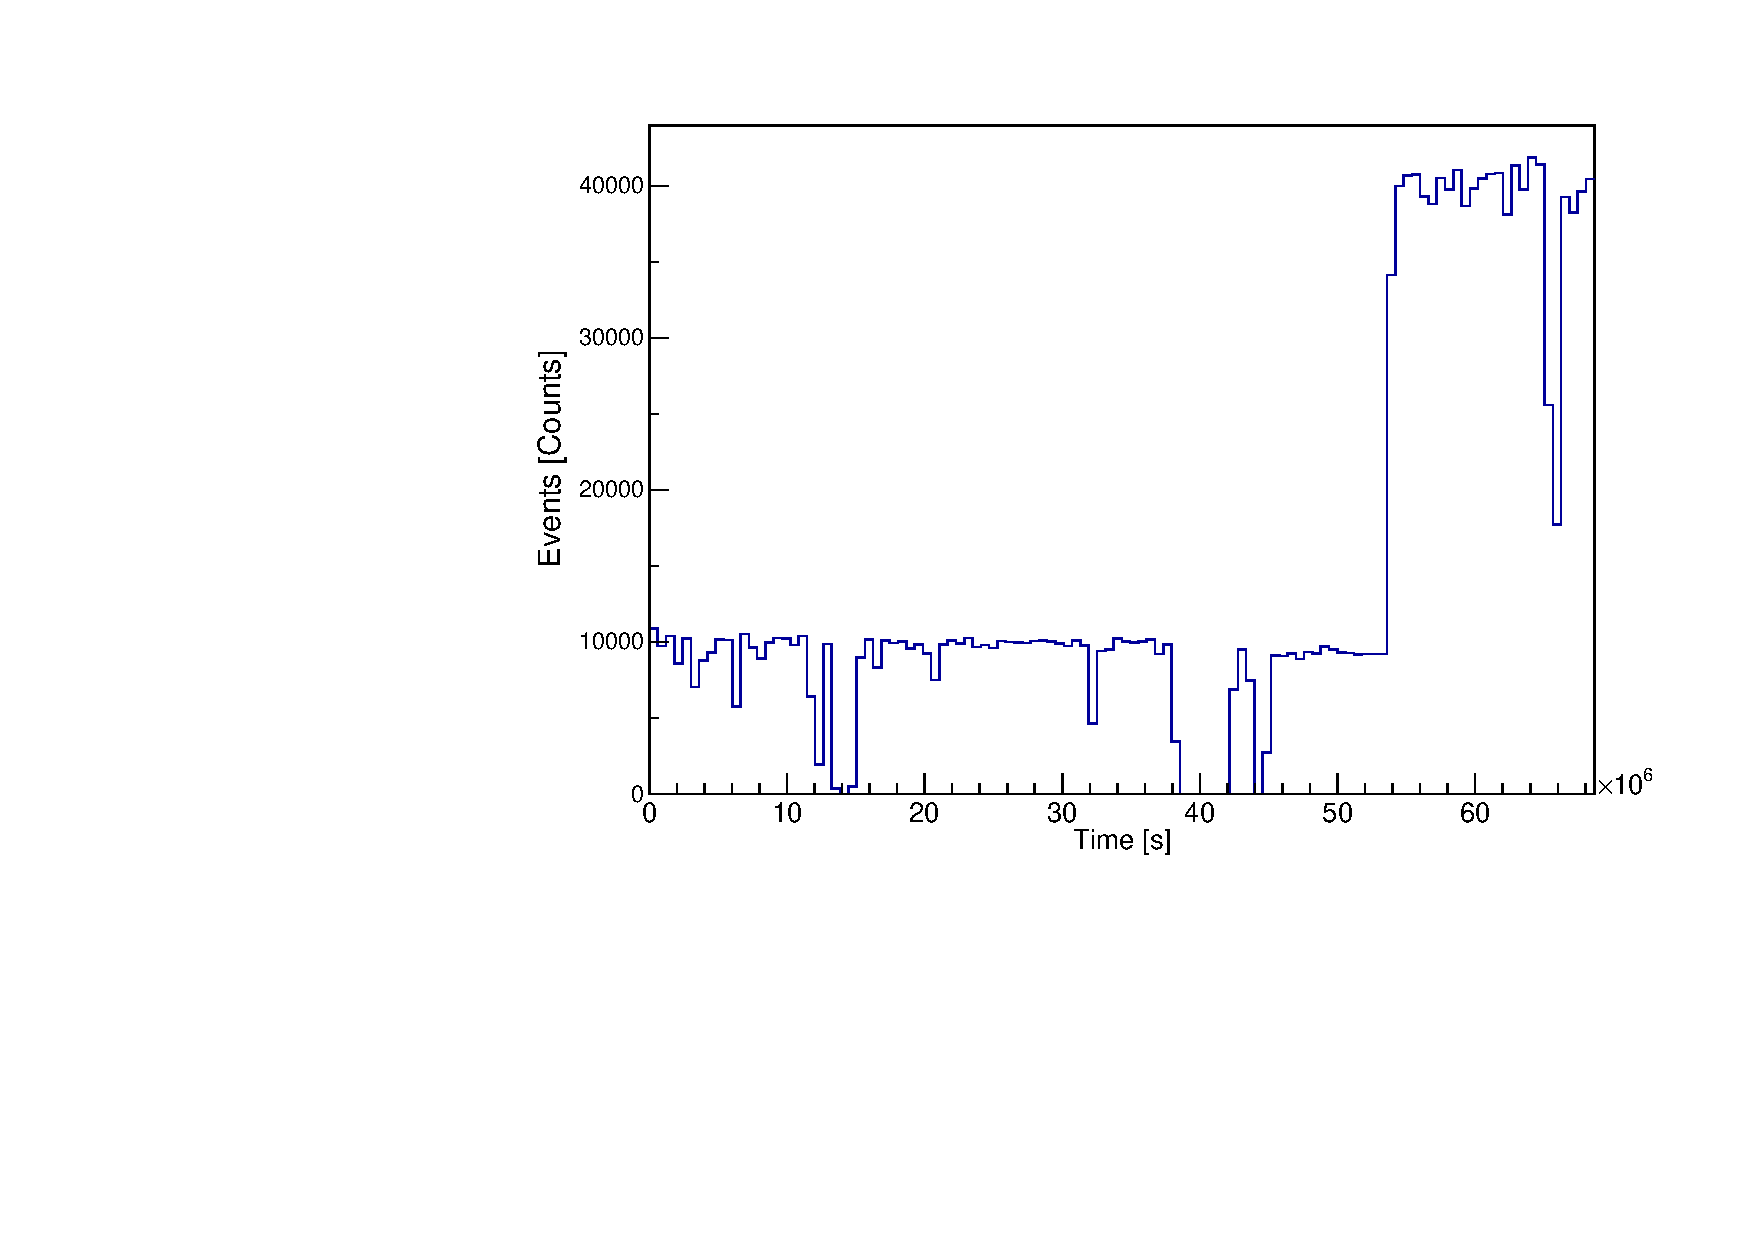
\includegraphics[width=\textwidth]{./Bilder/ZeitverlaufALLE.pdf}
		\caption{every event}
		\label{fig:ZeitAll}
	\end{subfigure}%
	\begin{subfigure}{.5\textwidth}
		\centering
		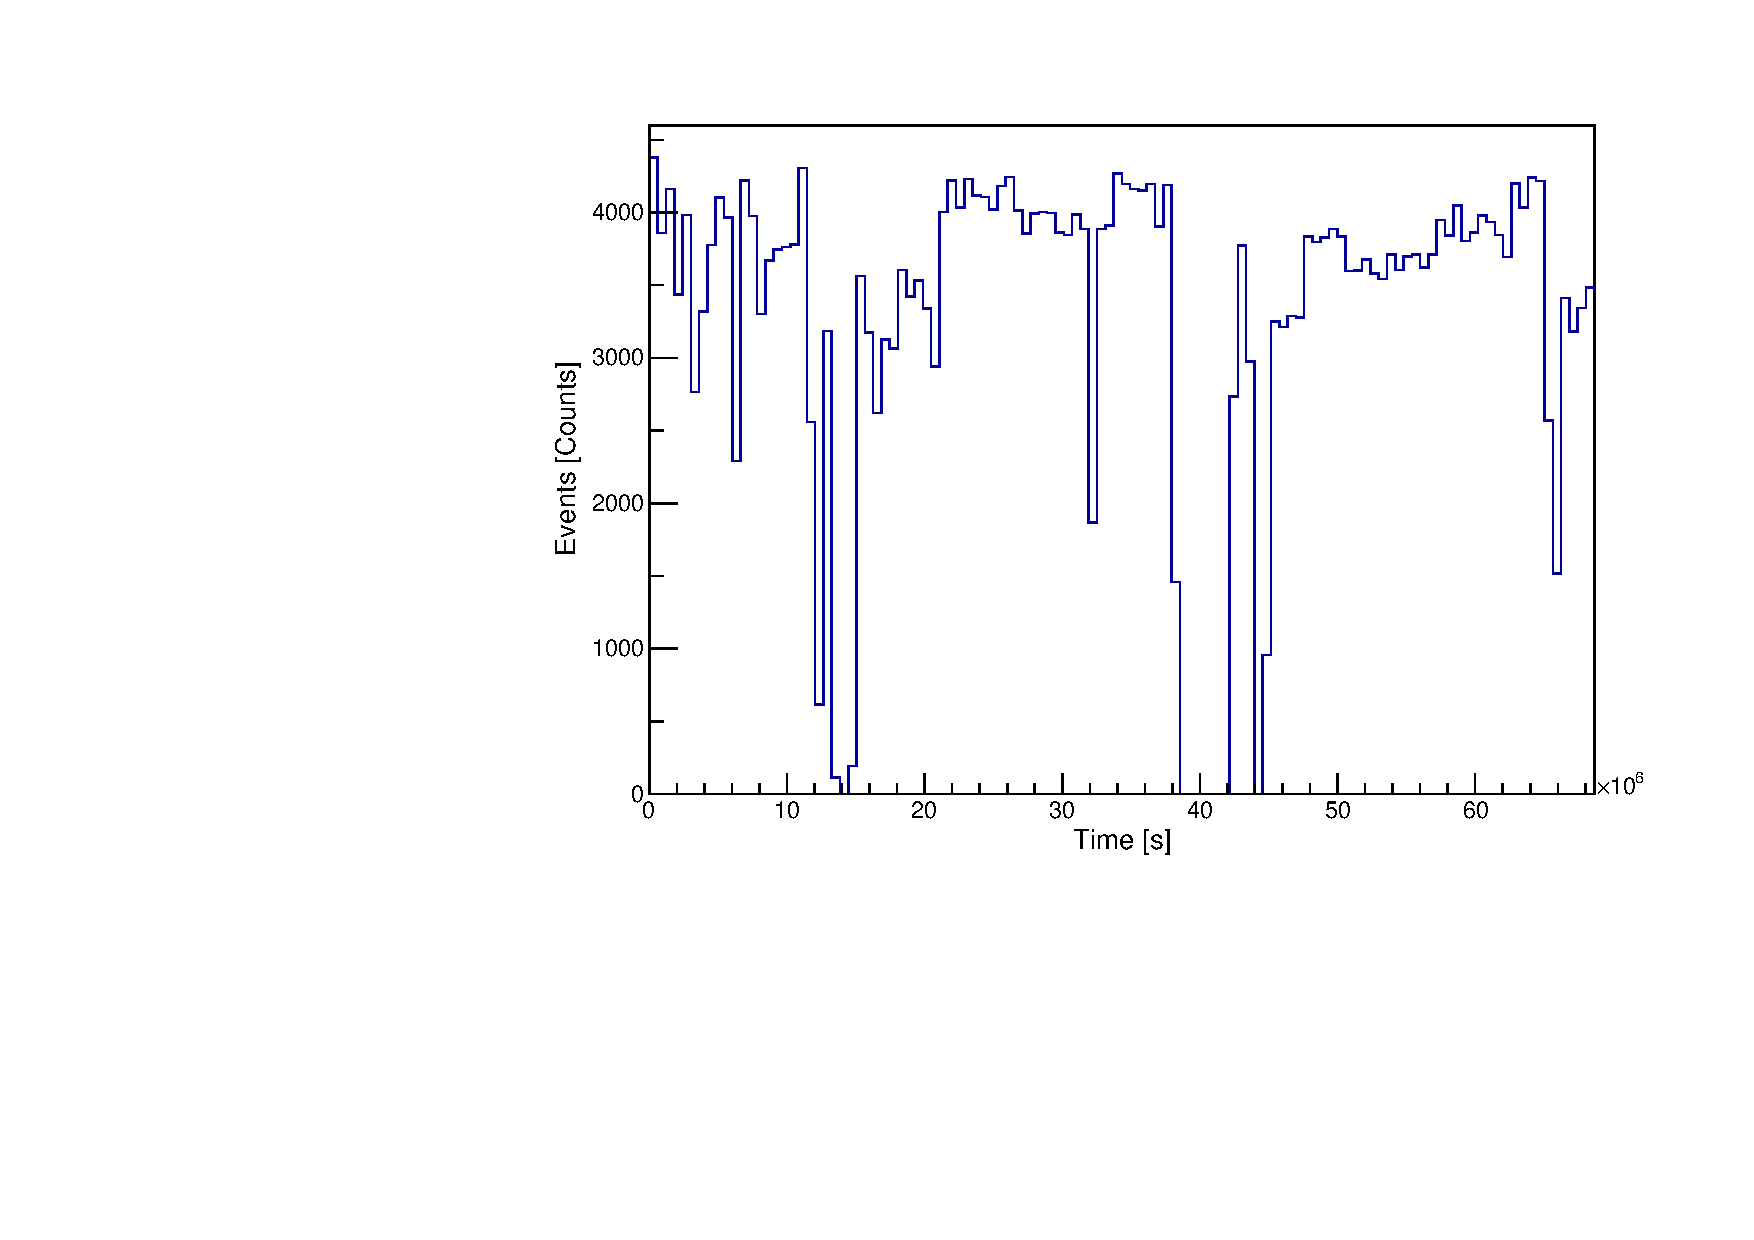
\includegraphics[width=\textwidth]{./Bilder/ZeitverlaufLimits.pdf}
		\caption{only energies between 200 and 400keV}
		\label{fig:ZeitLimits}
	\end{subfigure}
    \\
    \caption{Change of Intensity with time. In both figures are the amount of events measured in one week plotted over the whole time of \PII. In figure (a) no filters were imposed onto the displayed events while in (b) only those events are shown that have an energy between 200 and 400 keV. One can see that further precautions must be taken before an exponential decrease can be determined. }
\end{figure}

To determine the event rate one has to plot the amount of measured events over time in an event histogram with a suitable binning (see figure \ref{fig:ZeitAll}).
In this case a binning of one week per bin was chosen which results in about 114 bins for the 2.17 years of \PII.
As with the line count rate analysis, here we used only these events in the \ref{fig:ZeitAll} histogram where the Muon veto and the detector anticoincidence veto were not triggered.
When looking at the histogram for the first time two things jump into your eye.
Firtsly, there seems to be a great jump in the amount of events measured in the second half of \PII.
And secondly, there are times in which the amount of events measured drop to zero.
These two discontinuous changes to our expected outcome of an exponential decrease make it impossible for us to lay an exponential fit function throug the graph.
We therefor have to find a way to suppress them.
But for this to be done we first have to investigate where these discontinuities originate from.
\\

Firstly, we discuss the big jump in number of events measured.
This jump originates from the change of the lowering of the energy threshold on the 12.10.2017.
This reduction of the lower threshold dramatically increased the number of events measured.
Due to every detector having different characteristics, the limit was set for each detector individually.
Before the lowering the highest limit was set at about 140keV for the BEGes and at 185 for the COAX.
After the lowering all event with an energy of at least about 15keV could be recorded by all detectors.
For a more graphical representation, see the beginning of the spectra in figure \ref{fig:before} for all events measured before and figure \ref{fig:after} for all events after the lowering of the limit. 
This means that from the 12.10.2017 on a much higher event rate was measured just because more event were actually recored.
To work around this continuity problem all we have to do is limit our event used for the analysis to those that have a minimal energy of 200keV. 
While we are already at it we can also set up an upper limit on the energy.
Its purpose is to suppress events caused by isotopes with a higher end point energy than \Kr.
Even though they should only create a constant background, but their presence make a change in intensity harder to identify.
We therefor chose the upper limit to be at 400keV.
Theoretically the endpoint energy of \Kr is at 687keV, but the count rate towards the endpoint is that low that we would basically only include more constant background by setting the upper limit higher.
A new plot including only events between the energy limits of 200 and 400keV can be seen in figure \ref{fig:ZeitLimits}.
\\
\begin{figure}[t!]
	\centering
	\begin{subfigure}{.5\textwidth}
		\centering
		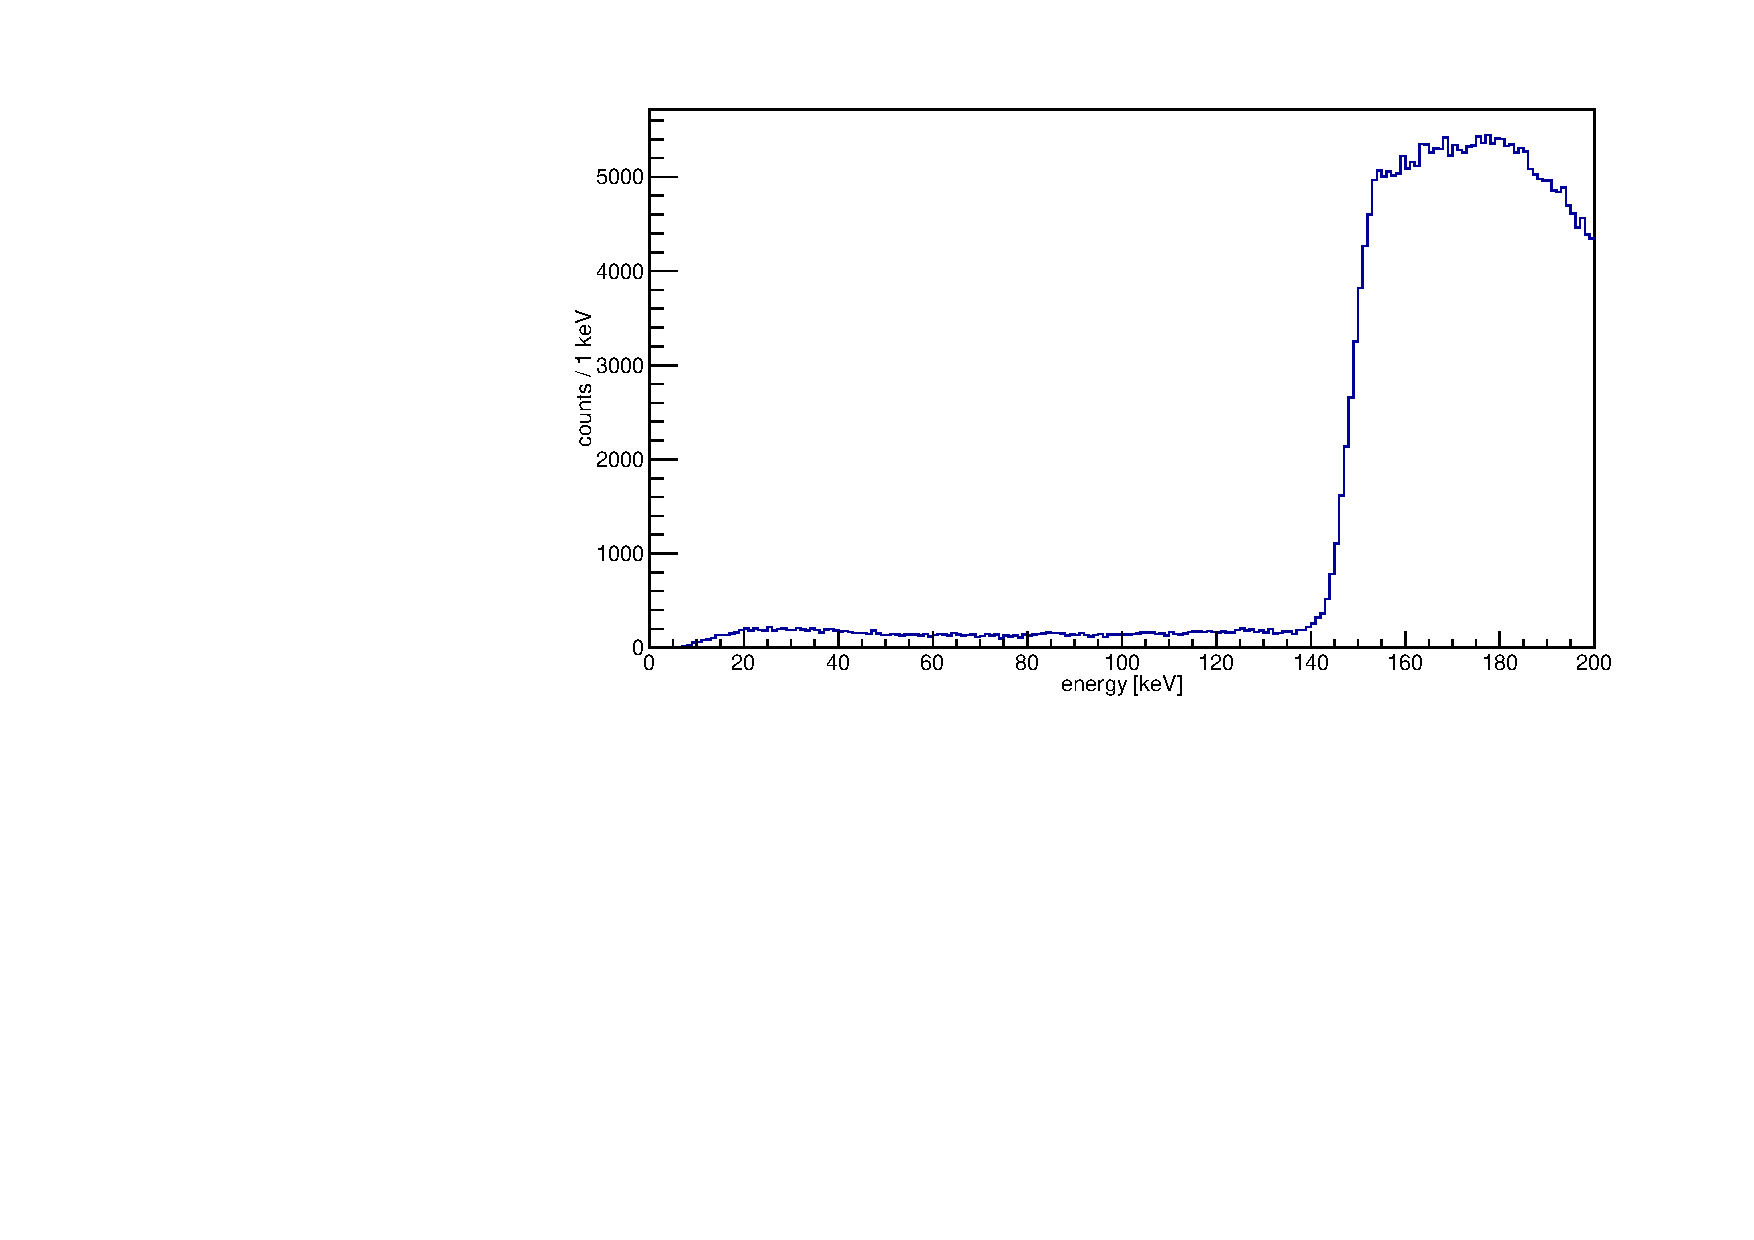
\includegraphics[width=\textwidth]{./Bilder/beforeTheFall.pdf}
		\caption{before}
		\label{fig:before}
	\end{subfigure}%
	\begin{subfigure}{.5\textwidth}
		\centering
		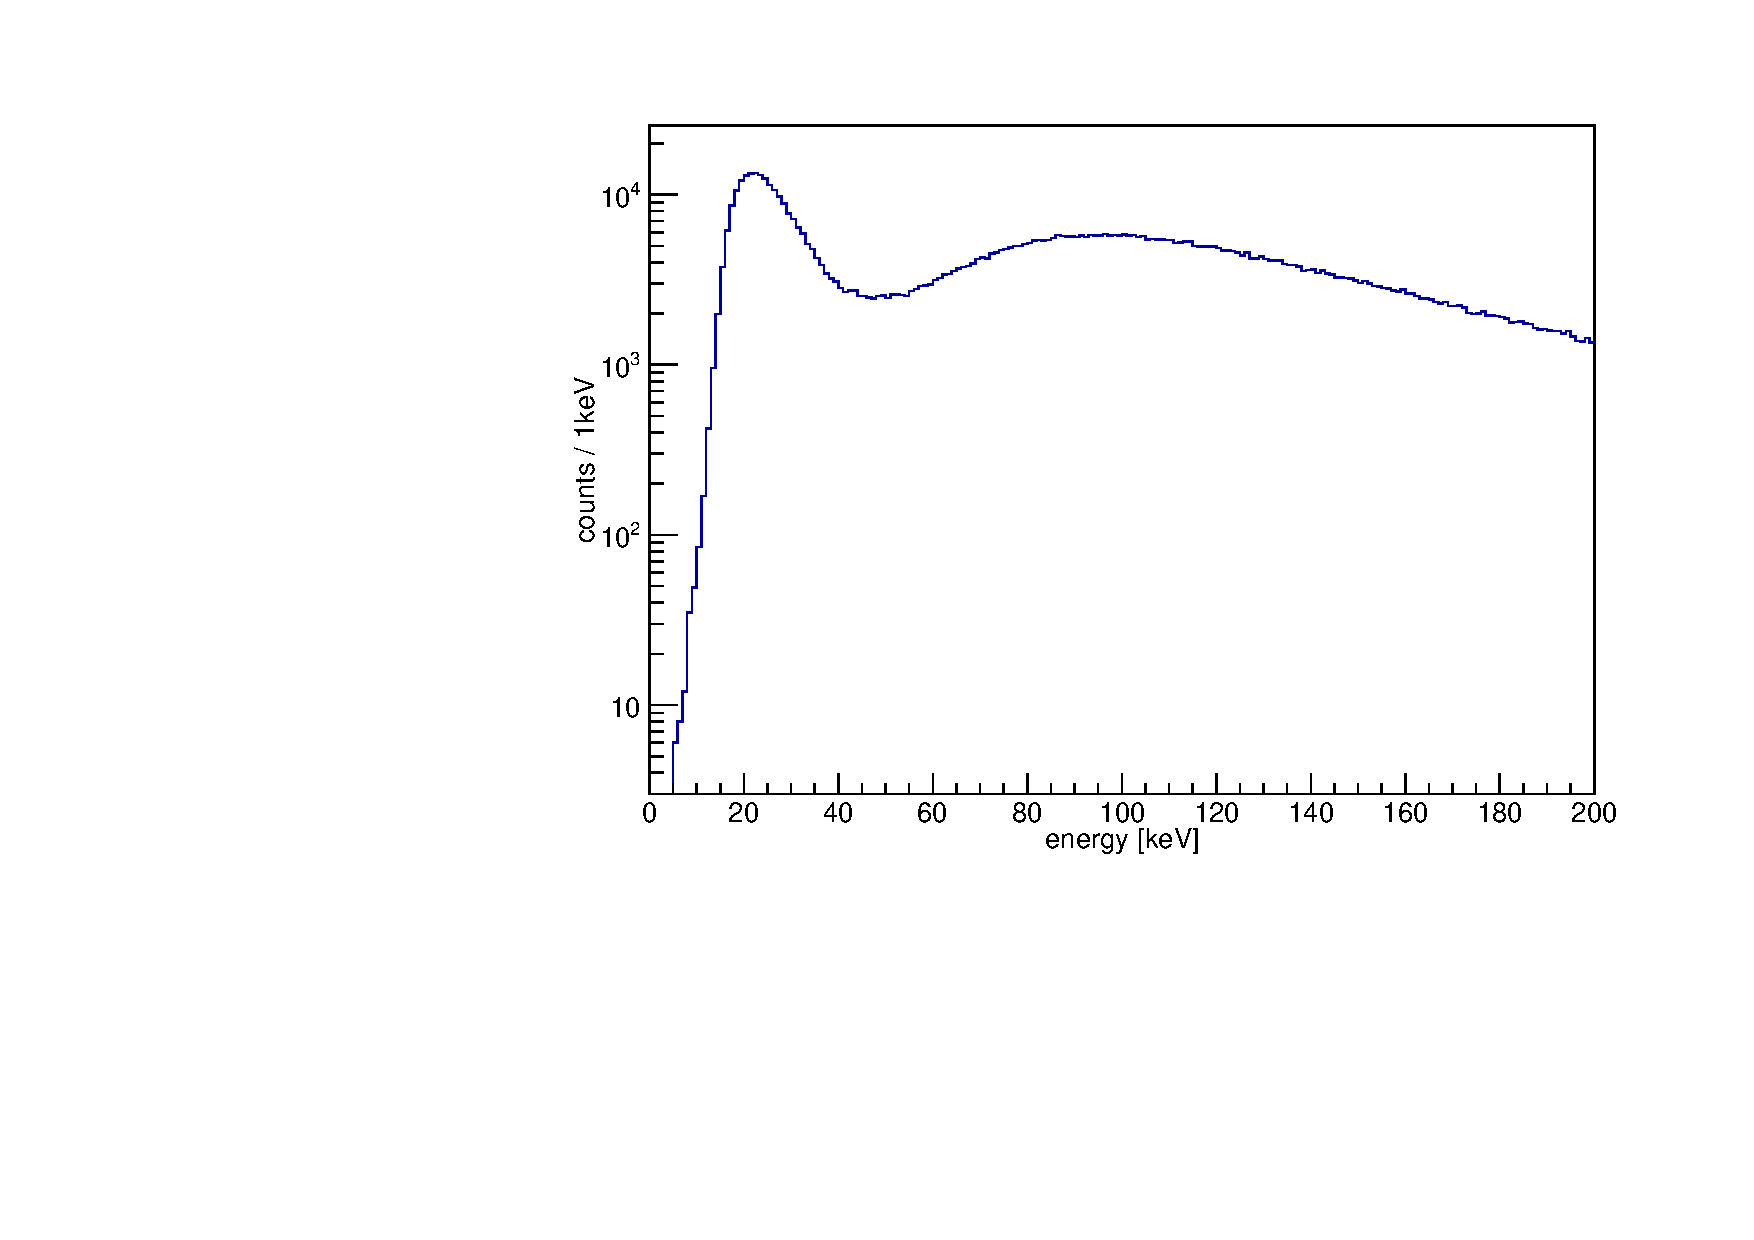
\includegraphics[width=\textwidth]{./Bilder/afterTheFall.pdf}
		\caption{after}
		\label{fig:after}
	\end{subfigure}
	\\
	\vspace{0.5cm}
	\caption{ }
	\vspace{0.5cm}
\end{figure}

The second discontinuous behavior originates from the same problem that we faced in the line count rate analysis.
Not all detectors were on all of the time and there were also time intervals in which no signal at all was recorded.
Due to the fact that some of the detectors were turned on or off over the time of \PII will result in discontinuous changes in the event rate because more or fewer events were able to be measured.
But this can easily be solved by only considering those events measured in a detector that was always turned on.
Which detector was always on over all of \PII can be seen in figure \ref in the appendix.
On the other hand due to there being time intervals in which no events were recorded the event rate drops discontinuous to zero there.
In section \ref{sec:CalcActiv} we solved this problem by calculating an effective measuring time for each detectors.
Here, however, we are not interested in an average measurement time over the entire \PII.
In this method we must find a way to weigh each individual bin of the event histogram with the corresponding effective measurement time of that bin.
This is where the test pulse signal comes in handy.
It is a clear indication of when exactly data was actually recorded.
This means that similar to the first method we can now determine effective measuring times of each time interval of the bins.
These mean measuring times can easily be calculated by plotting the test pulse signals in an histogram with the same binning as the event histogram and dividing each of these bins with the frequency of the test pulse of $f_\mathrm{TP} = 0.05\unit{Hz}$ (see figure \ref{fig:effectiveMeasuringTimes}).
The contents of these bins in the test pulse histogram correspond now to the respective measuring time in the binning intervals. 
\\

By dividing all bins of the event histogram by the corresponding bins in the test pulse histogram, you would get a new histogram showing the change of events measured in the time intervals of the bins (see figure \ref{fig:ChangeInEventRate}).
Or in other words, this new histogram shows us the event rate per week over all of \PII.
\\
\begin{figure}[t!]
	\centering
	\begin{minipage}{.5\textwidth}
		\centering
		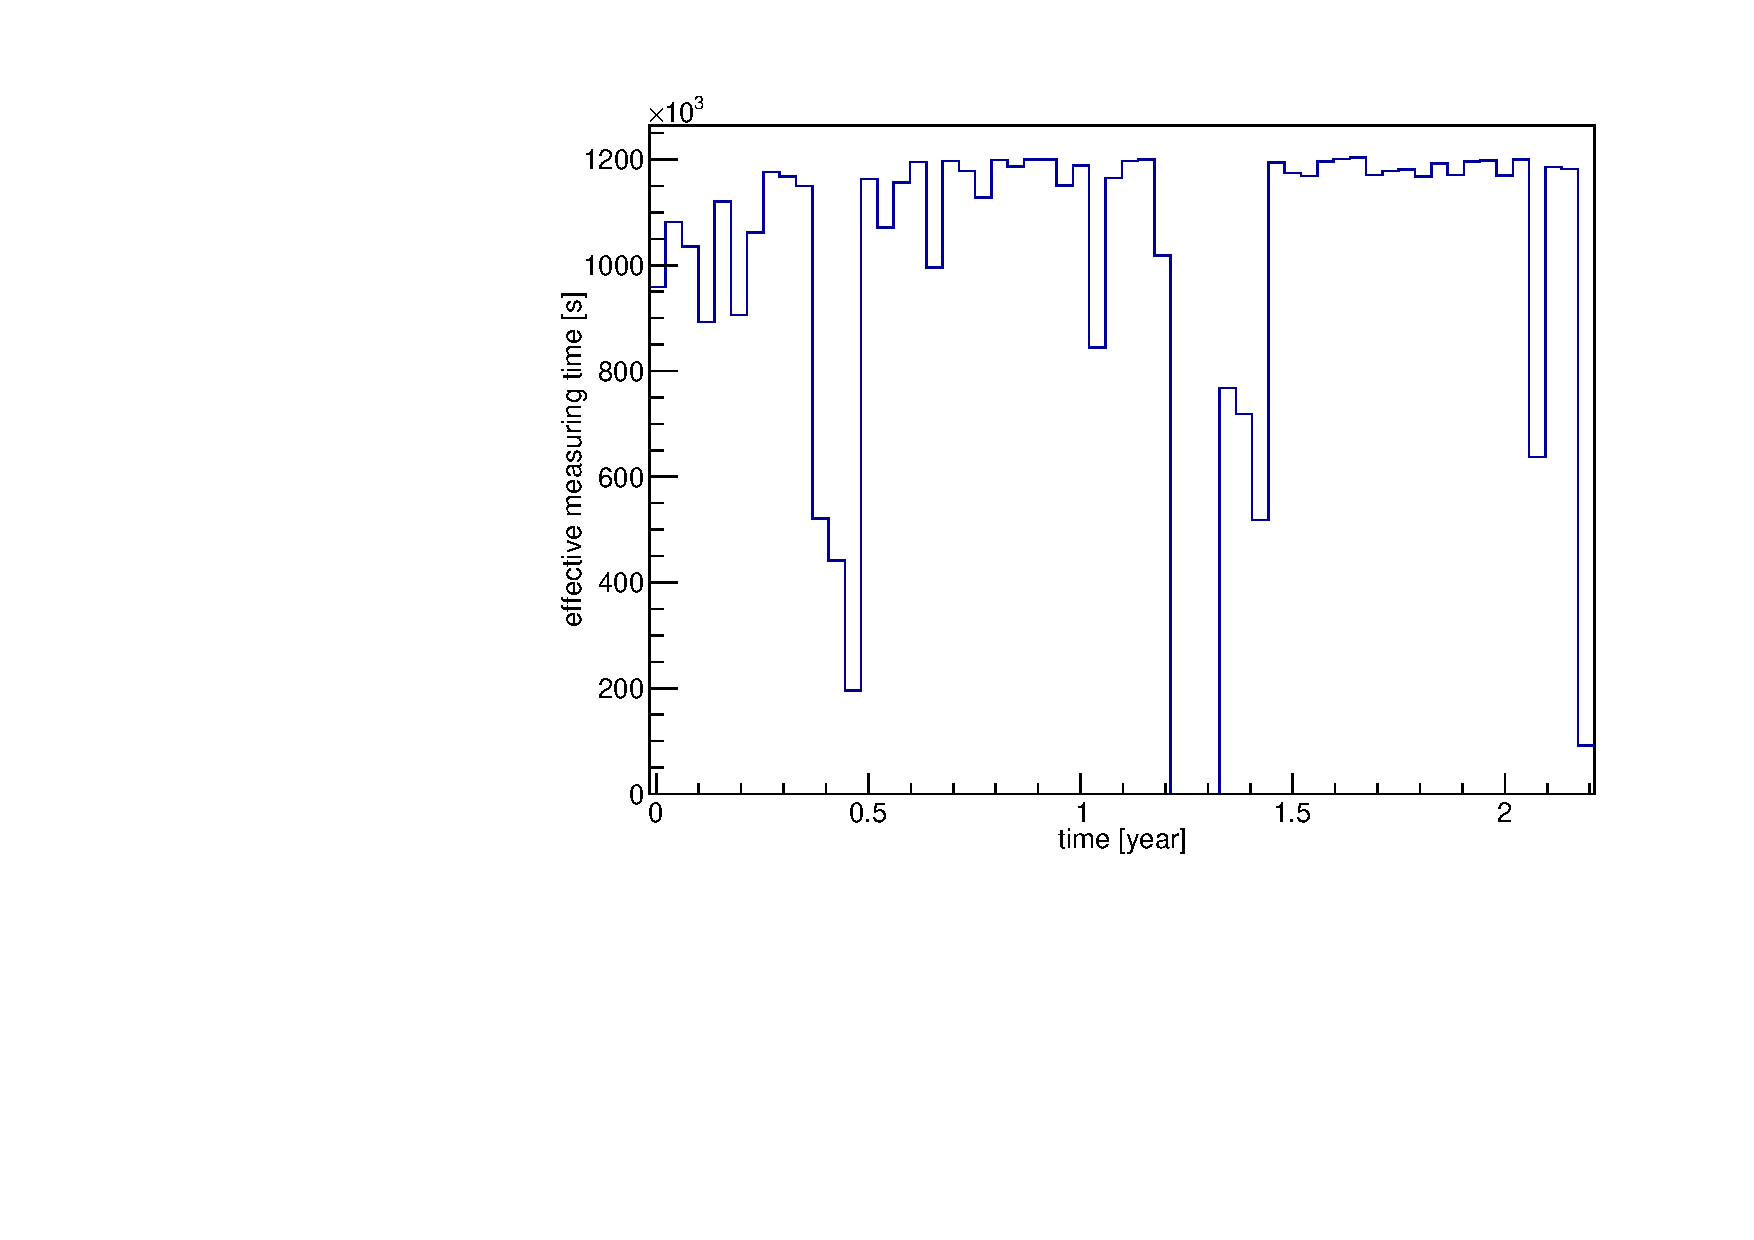
\includegraphics[width=\textwidth]{./Bilder/testpuler.pdf}
		\caption{effective measuring times}
		\label{fig:effectiveMeasuringTimes}
	\end{minipage}%
	\begin{minipage}{.5\textwidth}
		\centering
		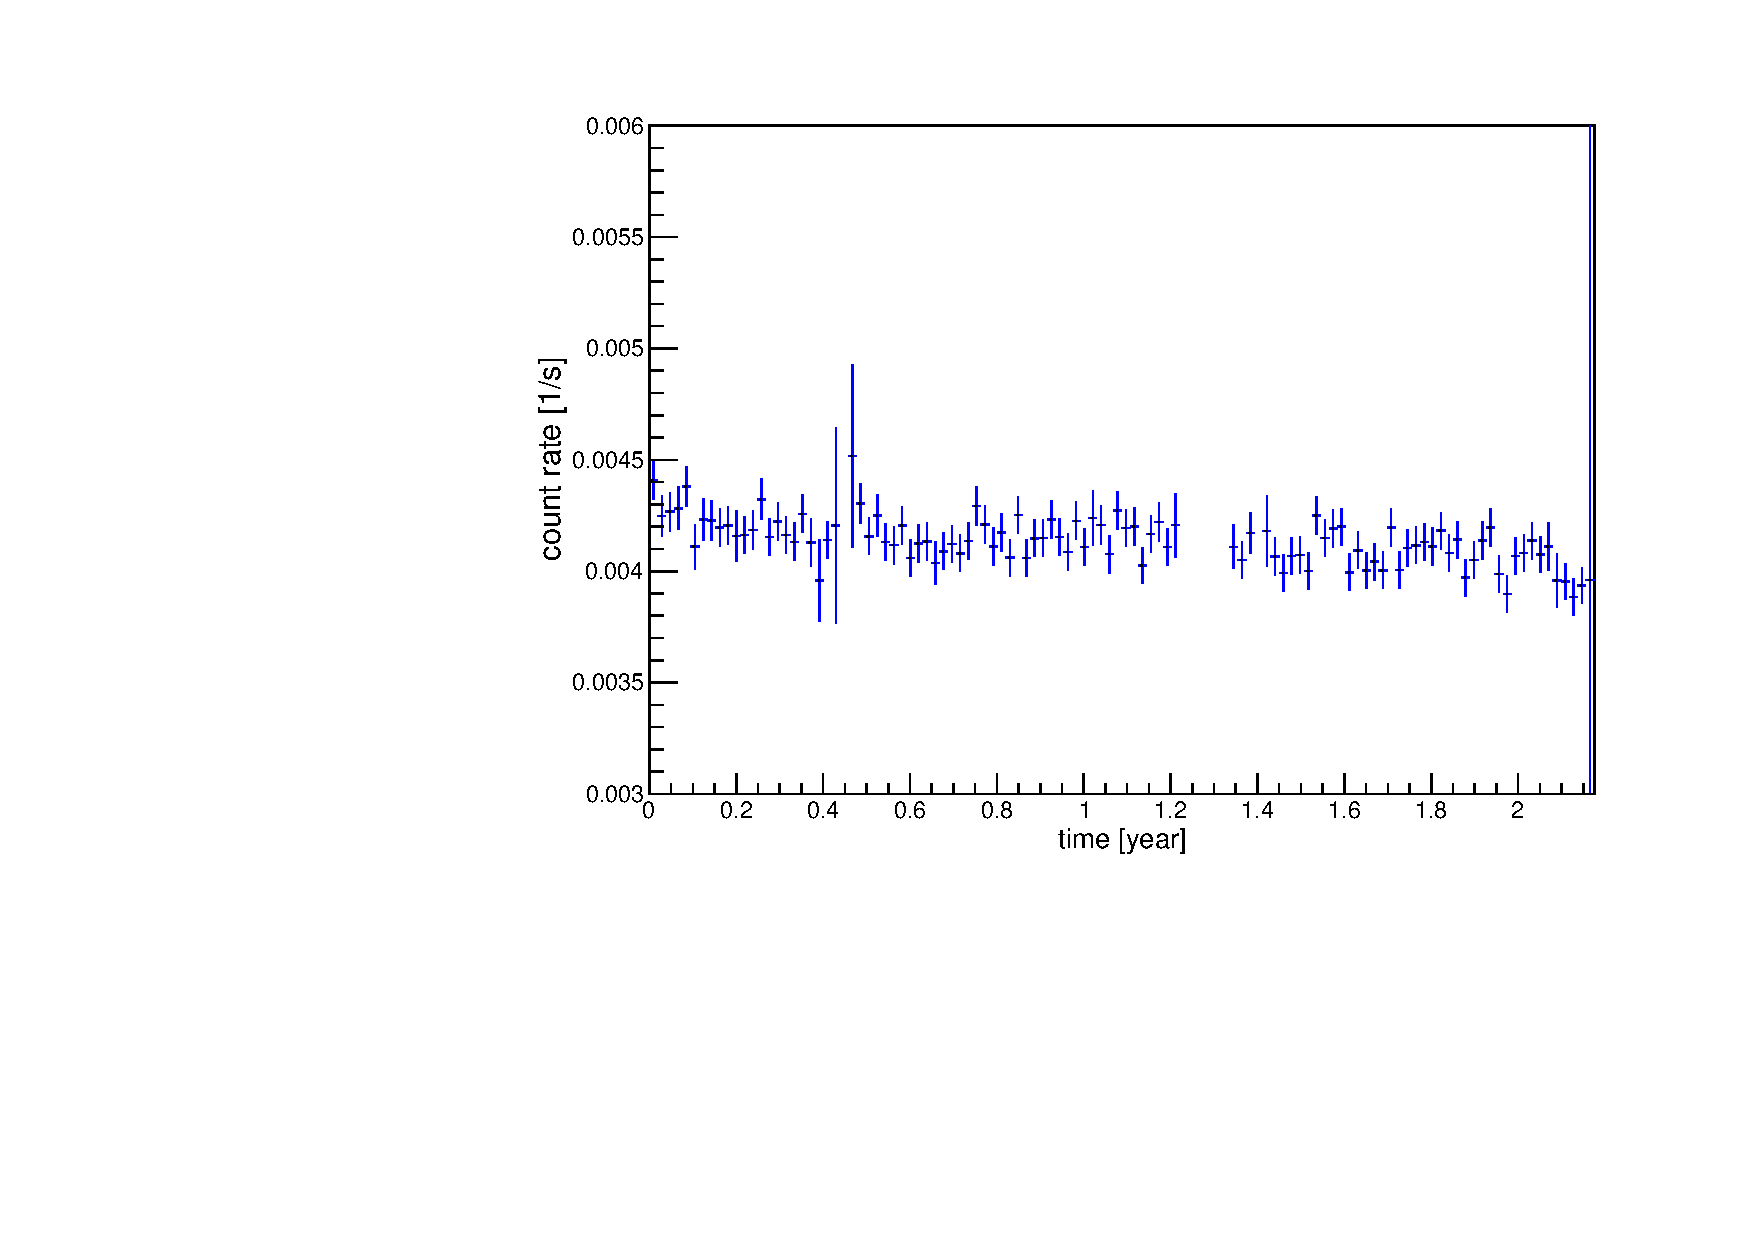
\includegraphics[width=\textwidth]{./Bilder/eventRate.pdf}
		\caption{after}
		\label{fig:ChangeInEventRate}
	\end{minipage}
	\\
\end{figure}

From this graph we now want to determine the exponential change in the event rate by applying an exponential fit function.
The exact fit function used is
\begin{equation}
\mathrm{f}(x) = \mathrm{A}\times\exp\left(-\frac{\log(2)}{\mathrm{B}} x \right) + \mathrm{C}
\label{equ:FitFilters}
\end{equation}
In this is A corresponding to the measured \Kr event rate of the decreasing function, B the half life of the decrease and C the constant event background rate.
Due to us exacting only \Kr to change over time we can already fix fit-parameter B to \(10.739\unit{y}\) which is the half life of \Kr and leaving the other two parameter relatively free.
From the resulting fit function (seen figure \ref{fig:ChangeInEventRateFit}) we get the fit parameters as seen in table \ref{tab:FitParZeit}.
The only parameter we need for our analysis is parameter \(\mathrm{A} = R_{\mathrm{count}} = \) being the \Kr event rate meaning that !!!!! events caused by \Kr decays could be measured every second.
Now that we have the \Kr event rate all we need now to determine the specific activity is the conversion factor from the measured events to the necessary \Kr decays in the liquid argon to cause this \Kr event rate.
As described above we need a new Monte Carlo simulation for that.
What this simulation actually simulates and how we determine the conversion factor from it is the topic of the following section.


\begin{table}[t!]
	\centering
	\begin{tabular}{|l|r|}
		\hline
		Name	& Value  \\ 
		\hline
		A  &	(17.844639 \(\pm\)	3.179471)\\	
		\hline
		B  &	(513.838989 \(\pm\)	0.665171)\\	
		\hline
		C  &	(0.828315 \(\pm\)	1.377836)\\
		\hline
	\end{tabular}
	\caption{Fit parameters of fit function \ref{equ:FitNoFilters} applied on the spectra of the respective detectors.}
    \label{tab:FitParZeit}
\end{table}

\begin{figure}[t!]
	\centering
	\ifmakefigures%
	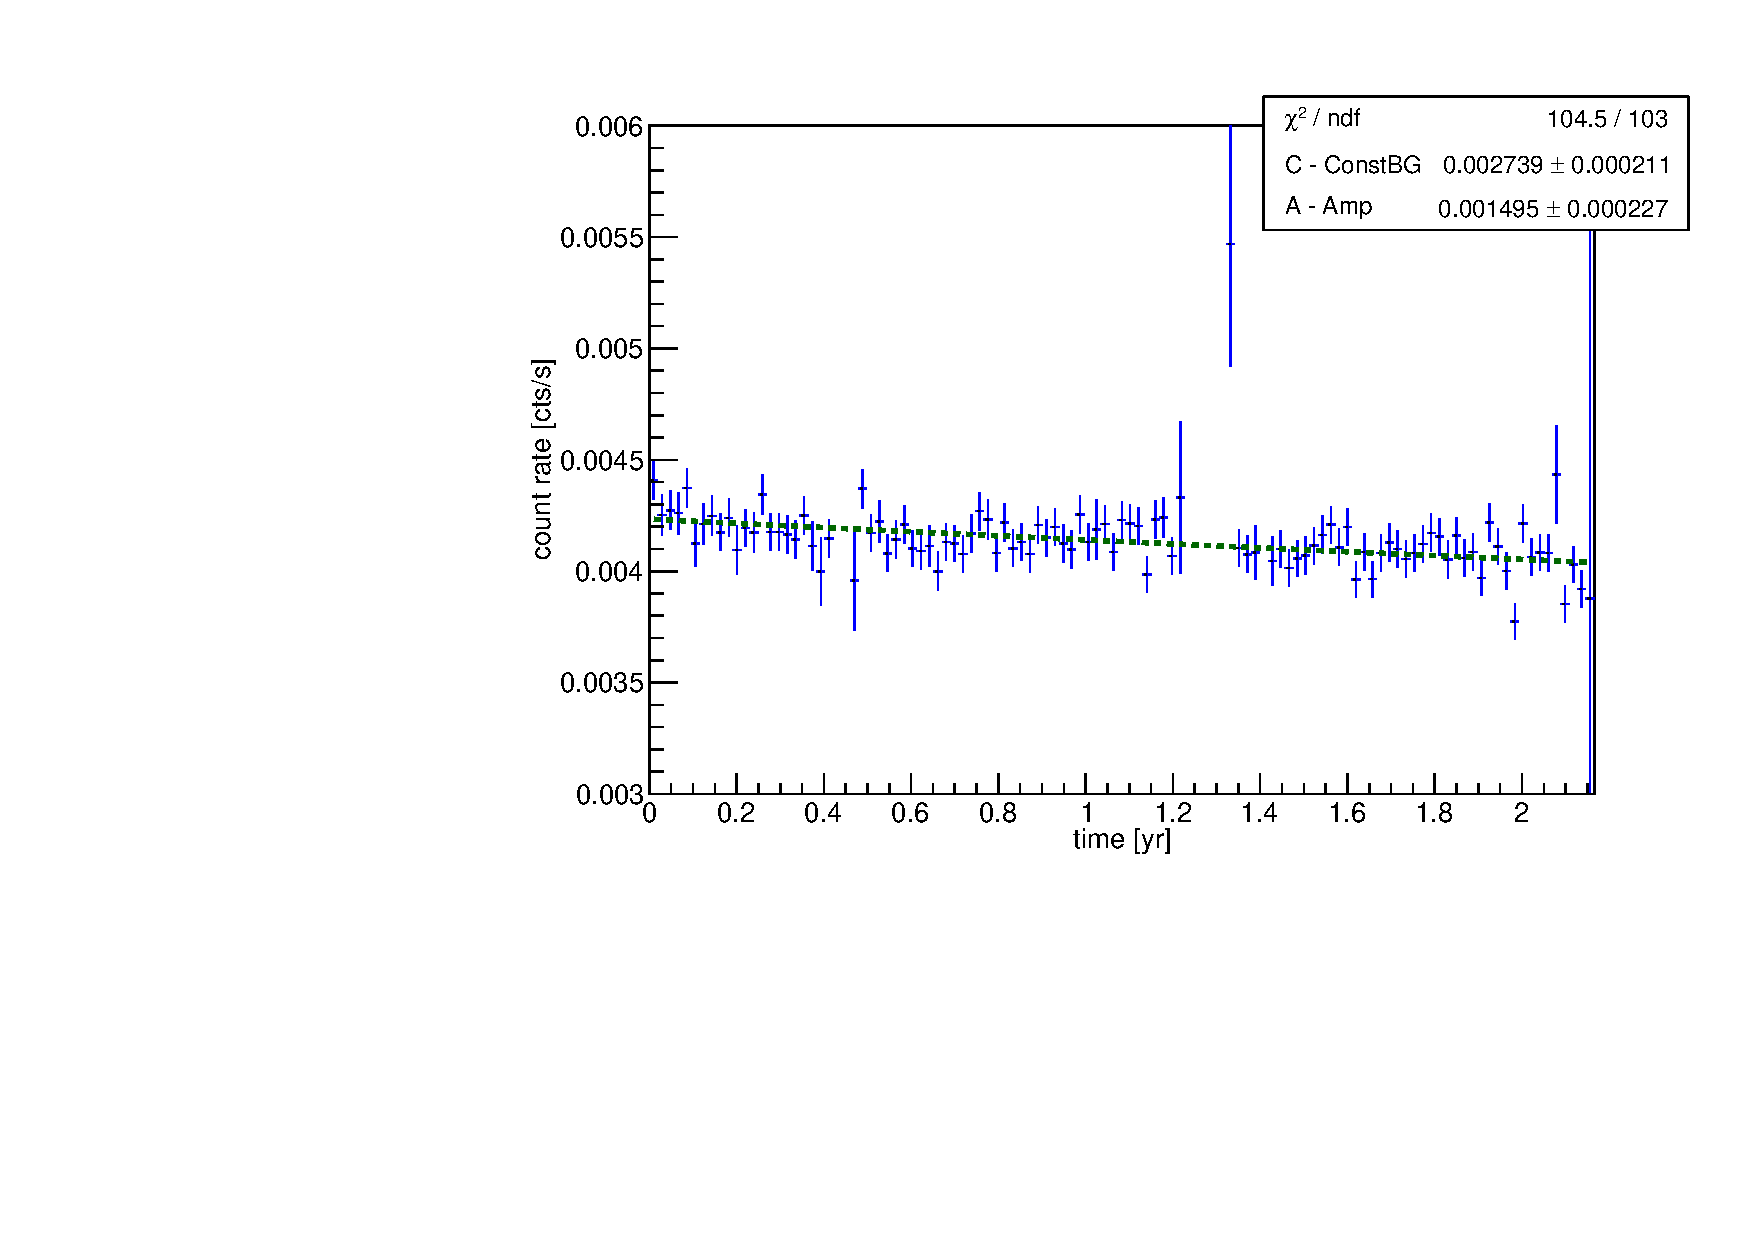
\includegraphics[width=100mm]{./Bilder/eventRateFit.pdf}
	\fi%
	\caption{effective measuring times}
	\label{fig:ChangeInEventRateFit}
\end{figure}%
\begin{figure}[t!]
	\centering
	\begin{minipage}{.5\textwidth}
		\centering
		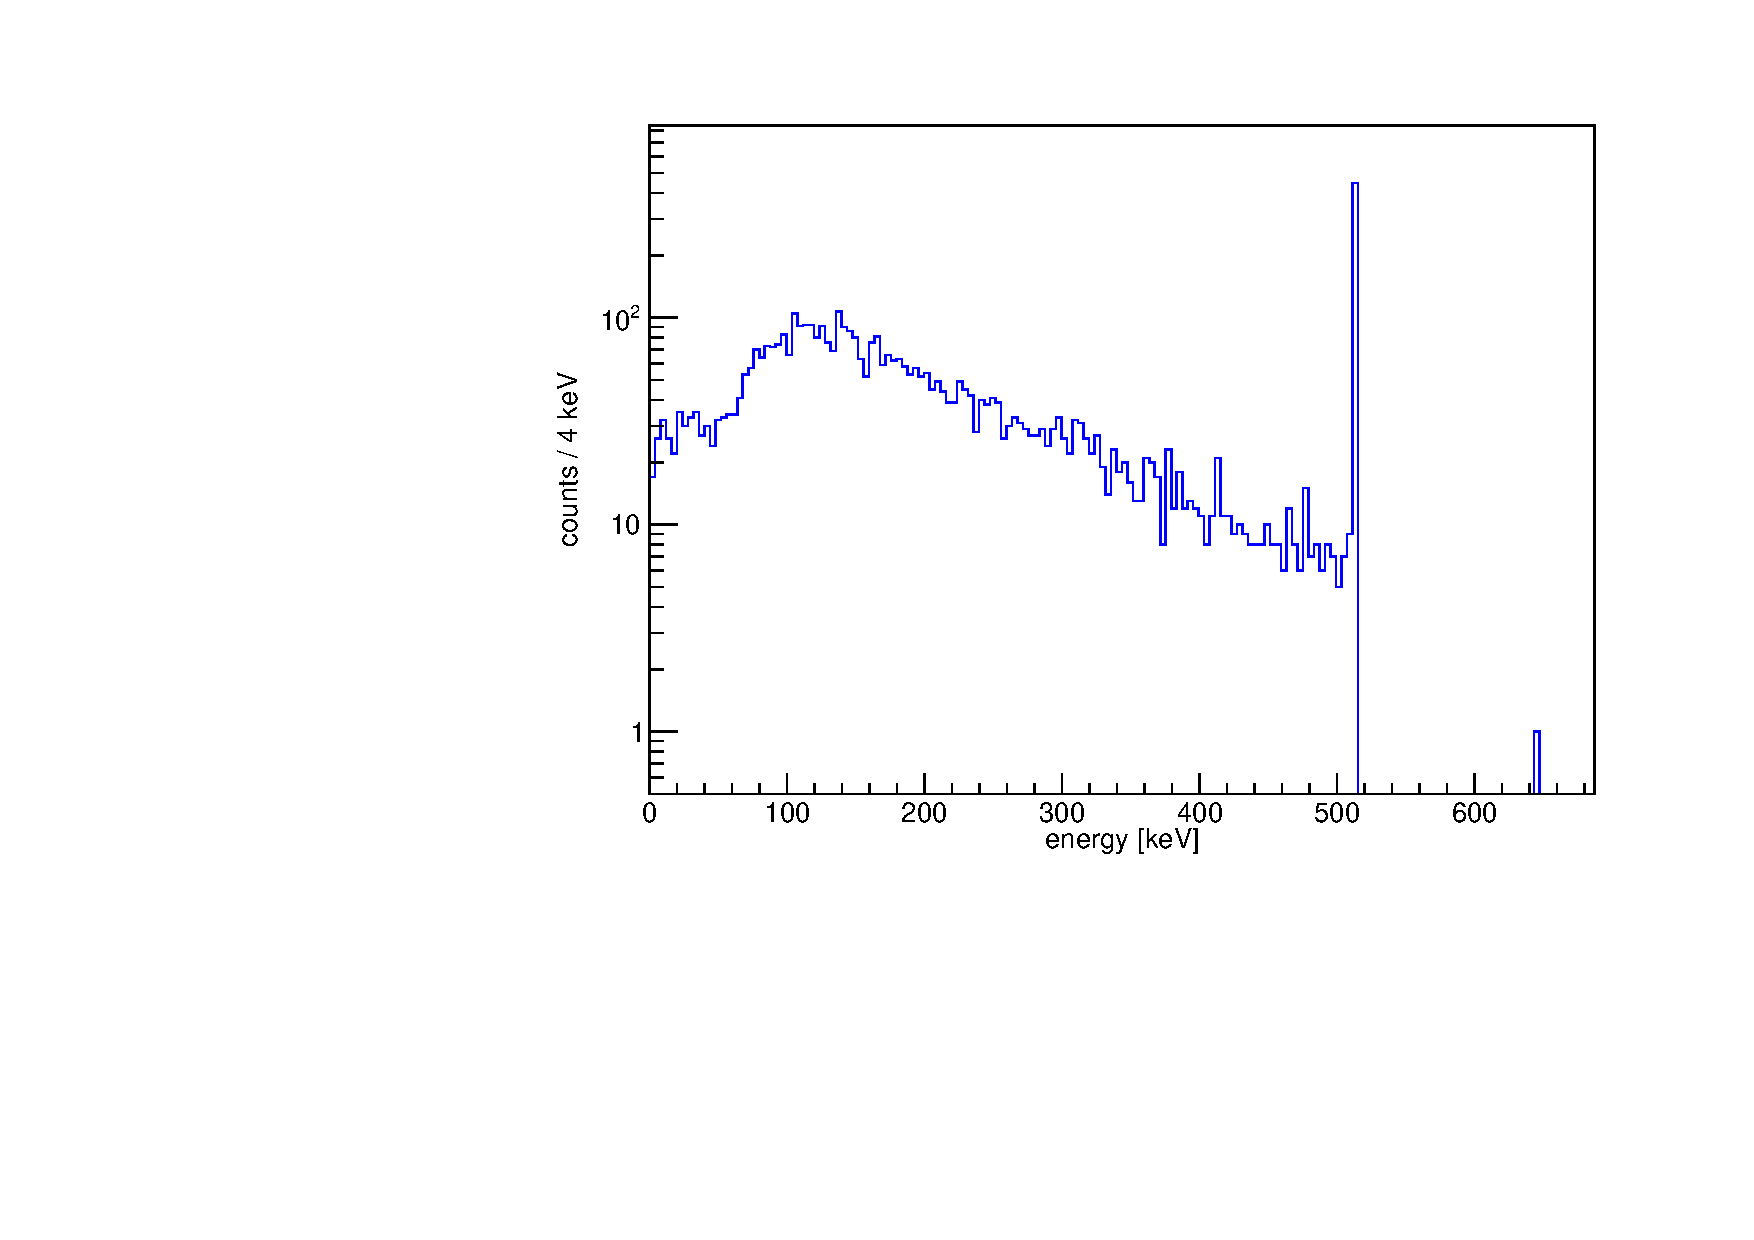
\includegraphics[width=\textwidth]{./Bilder/Sim1Phasenraum.pdf}
		\caption{after}
		\label{fig:Sim1Spektrum}
	\end{minipage}%
	\begin{minipage}{.5\textwidth}
		\centering
		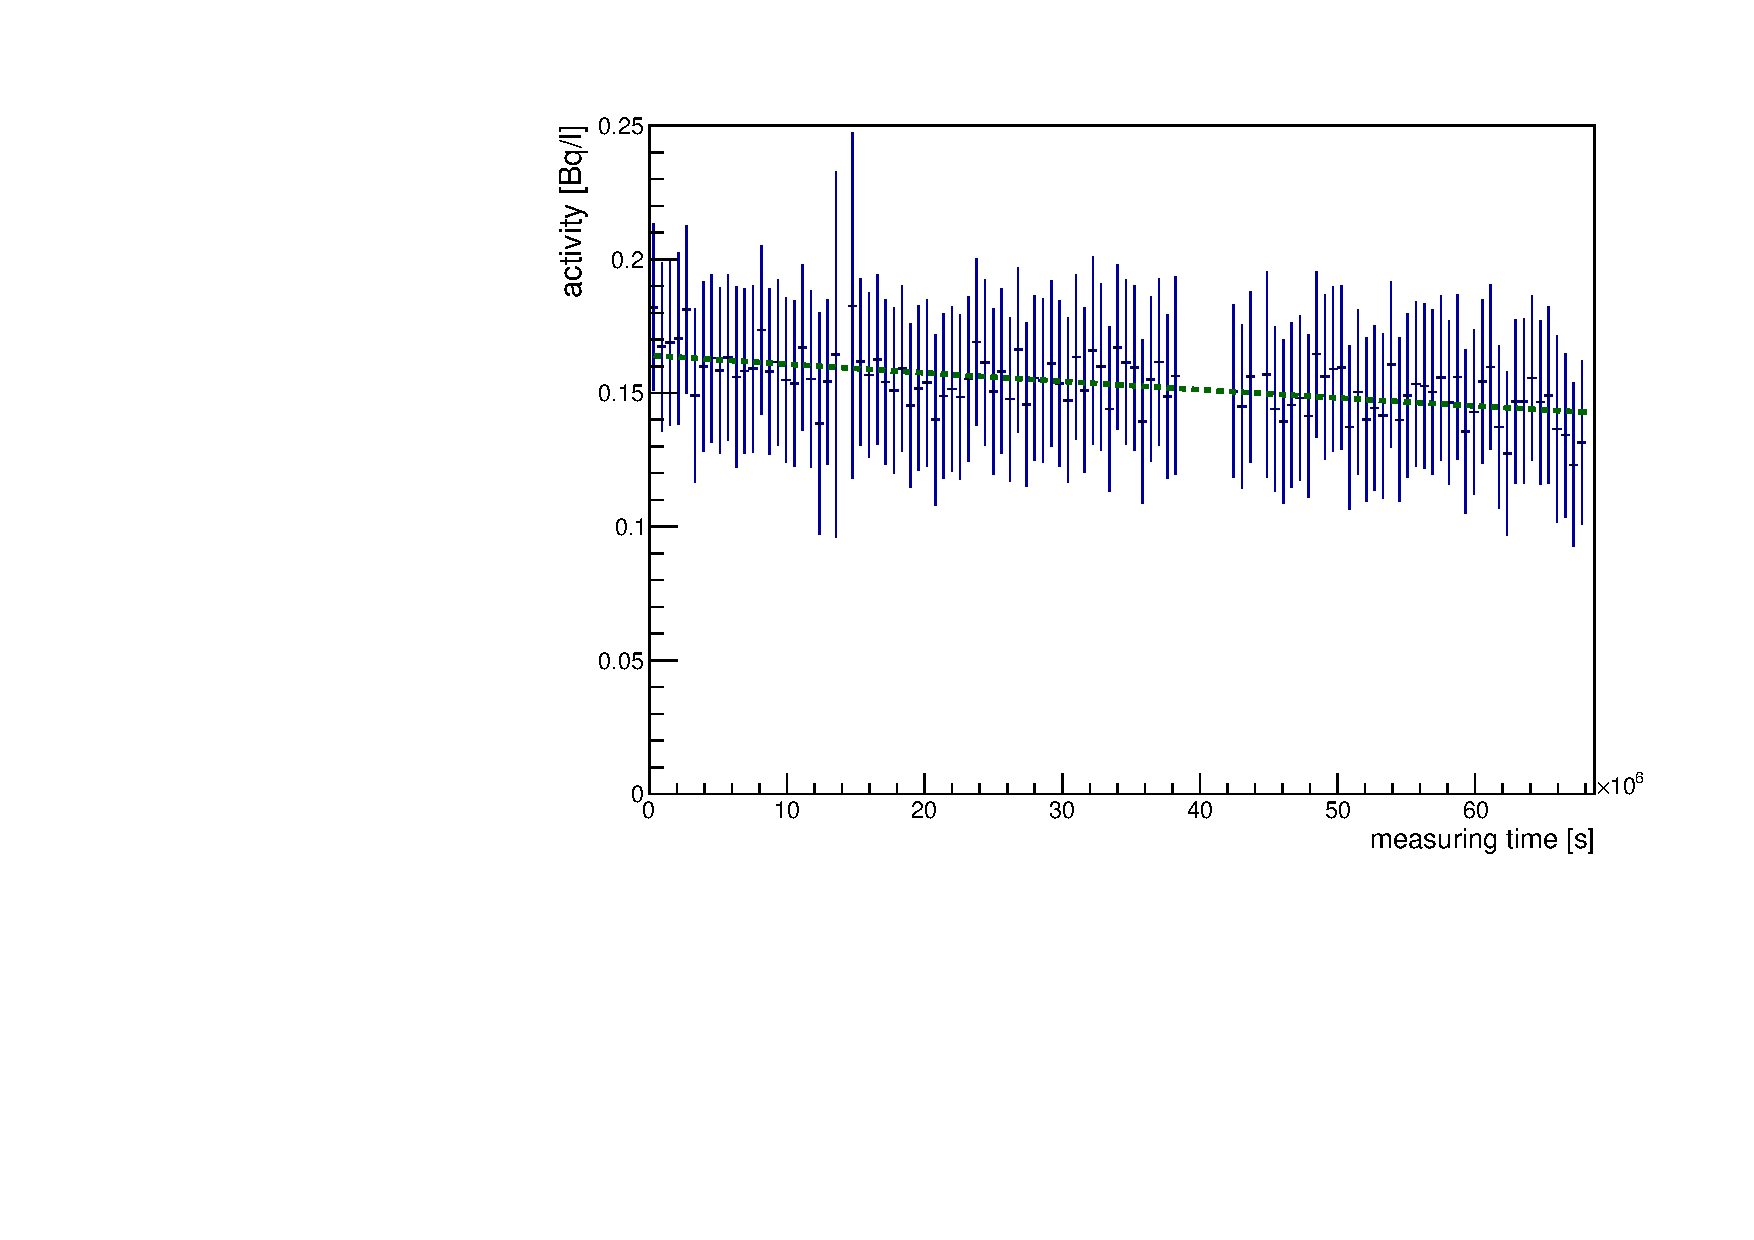
\includegraphics[width=\textwidth]{./Bilder/Aktivitaet.pdf}
		\caption{specific activity of \Kr over time}
		\label{fig:activity}
	\end{minipage}
\end{figure}
\section{Monte Carlo simulation}
\label{sec:MonteCarlo2}


!!!!! zur deadlayer noch genauer was heraussuchen !!!!!

To calculate this conversion factor we have to apply the same process as in the line count rate analysis.
Just that we this time don't simulate the emission of photons with an energy of 514keV in the liquid argon but rather simulate the actual \Kr decays themselves.
But a problem is, that we can expect the detector efficiency of \Kr to be very small.#
This is because the electrons probability of being detected is being suppressed by the fact the detectors themselves have a small dead layer of germanium around them.
If an electron is captured in this dead layer it will create no signal that could be recored even though it hit the detector.
On the other hand if a photon hits the detector it is very likely to deposit all of its energy inside the active detector area due to it being able to transmit further into the detector.
It also has to be considered that only those decays will be considered by us that made their event in one of the detectors that was always on.
Every other decay that made an event in another detector will be discarded making the detector efficiency even smaller. 
Because of this low expected detector efficiency we have to simulate a much higher amount of decays than photons were emitted in the other simulation.
\\

In this simulation we simulated N = 1 billion \Kr decays in a volume of again $V_{sim} = 17.65 \mathrm{m}^3$.
Due to the massive amount of simulated events only those decays were saved in which an event has been measured.
These events created a combined spectrum of the emitted electrons plus the photons emitted from the excited \nuc{Rb}{85m} as seen in figure \ref{fig:Sim1Spektrum}.
If you compare this spectrum with the one calculated for the other Monte Carlo simulation we can see these two spectra look very much alike.
But this would mean that the majority of the measured events must have been caused by the photons of the \nuc{Rb}{85m} relaxation.
That would also mean that almost none of the electrons emitted in the beta decay of \Kr created any signal.
This is actually an advantage for us.
If the majority of the measured events were created by electrons then we would have to apply a correction onto our detector efficiency.
This is because of a weakness of the simulated detectors.
The dead layer of the actual detectors isn't known that well which is why the simulated detectors can only work with an assumptions of the actual dead volume of the detectors.
Unfortunately, it's hard to correct the determined value for this weakness.
We are therefor in luck that the 514keV photons are responsible for the majority of event in the spectrum.
In this case no such correction has to be applied.
\\

But this conclusion of photons being the main cause of the spectrum assumes that in both simulations the same environmental conditions were simulated.
Whether this is true or not can easily be determined by looking at line count of the characteristic 514keV peak.
In the case of the first simulation an amount of 10179 events were measured by the BEGe detectors in the 514keV peak with a decay density of about 2832 $\unit{photon}/\unit{l}$.
On the other hand in the second simulation only 817 events were measured with a decay density of 56640$\unit{decay}/\unit{l}$.
But one has to consider that in the case of the first simulation only the photons of the \nuc{Rb}{85m} relaxation were emitted and \Kr only decays into this exited state with a probability of 0.434$\%$.
The effective decay density of the first simulation is therefor about 652511 $\unit{decay}/\unit{l}$.
To compare these two line counts, we now have to scale one of the two values so that they would theoretically have had the same decay density.
By applying the scale of $\frac{56640}{652511}$ onto the amount of events in the 514keV peak from the first simulation you get a adjusted value of 884 events.
The fact, that this value is roughly the same size as the value 817 form the second simulation, proves, that a similar environmental situation must have been simulated.
This conclusion also justifies retroactively the simplification in the first simulation of only emitting photons to replace the actual decay could be done.
\\

Now to calculating the conversation factor from this simulation.
Like we need the amount of events measured in the range of interest.
In this case we determine an amount of $\Delta$N = (1438$\pm$38) events in the spectrum that deposited an energy between 200 to 400keV.
With the absolute amount N of decays simulated we determine a detector efficiency of
\begin{equation*}
    \epsilon_{\beta} = \frac{\Delta \mathrm{N}}{\mathrm{N}} = (1.438\pm0.038)\times10^{-6} \frac{\unit{events}}{\unit{decay}}
\end{equation*}
This values says that any decay in the liquid argon has a probability of $\epsilon_{\beta}$ to be detected by one of the detectors that was always on.
With this value we can again calculate the volume independent conversation factor
\begin{equation*}
    \frac{1}{\epsilon_{\beta} V_{sim}} = (39.38\pm1.04) \frac{\unit{decay}}{\unit{events} \times l }
\end{equation*}
\\

With this conversation factor we can now also calculate the specific activity of \Kr.
By applying equation \ref{equ:activityAt0} and feeding it with the values found we result in an specific activity of $a = (0.0614\pm0.0419) \frac{\unit{Bq}}{\unit{l}}$ at the start of Phase II.

\begin{equation}
    a(t=0) = \frac{R_\mathrm{count}}{\epsilon_{\beta} V_{sim}} 
    \label{equ:activityAt0}
\end{equation}

We can get back to the graph \ref{fig:ChangeInEventRateFit} and apply the same formula to each of its values and the fit function.
The resulting graph can be seen in figure \ref
Because we want to compare this value to the specific activity found in the line count rate analysis, we have to now calculate the mean specific activity over all of Phase II.
This can easily be done by integrating an exponential decay function over all of \PII and then dividing it by 2.17 years.

\begin{equation*}
    \bar{a} = \frac{1}{2.17\unit{y}} \int_0^{2.17y} a(t=0)\times\exp \left( \frac{\log(2)}{T} t \right) \mathrm{d}t
\end{equation*}
with T being the half life of \Kr.
This results in an mean specific activity of $ \bar{a_{2}} = 57.294 \frac{\unit{mBq}}{\unit{l}}$.
\\

If you now compared this result with the specific activity found in the line count rate analysis you will realize that there is a problem.
The mean specific activity of all investigated detectors found in the first method had a value of $\bar{a}_{1} = (5.08\pm0.857)\times10^{-4}\frac{\unit{Bq}}{\unit{l}}$.
Compared to this is the value determined here two orders of magnitude bigger.
This is problematic.
But in actuality we could have seen this problem coming.
Because if we would expect the amplitude of the function shown in figure \ref{fig:activity} to be in the same order of magnitude as the other activity we determined, no real change should be seen over the uncertainty.
The critical question are now: 
Which of the methods is faulty, which of the assumption we used was wrong and can we still make a statement about \Kr specific activity from the problematic approach.
These question will be answers in the following section.
\\


\section{Discussion}
\label{Discussion}

The biggest advantage of the line count rate analysis compared to the second method is that in its case the investigated effect can only originate from \Kr and no other isotope.
Because of this the likelihood of its determined value being the actual specific activity is relatively high.
By comparing the results of the first method with those of the WARP and Darkside experiments, we have already seen that the specific activity of \Kr is lower than in all other experiments.
The second method however has the problem that theoretically every other isotope that is residual in the liquid argon contributes to the investigated change over time.
It can therefor be very likely that our mistakes lies in the assumption that all contribution of any other isotope to this change can be ignored. 
In the beginning of this chapter we already discussed all of the isotopes that are the most probable sources of error.
We already mentioned there that any contributions from \nuc{Ar}{39} and \nuc{Po}{210} can be disregarded due to their either high half life or their high mean kinetic energy of the escaping particle.
But as it was already indicated there, it might be necessary to discuss the influence of \nuc{Ar}{42} further.
\nuc{Ar}{42} has a half life of 32.9 y which is in the same order of magnitude as the half life of \Kr.
Therefore, we can expect to see a change in its activity over the course of \PII of about 4.4$\%$ of its absolute specific activity.
With an specific activity big enough one could expect this isotope to be responsible for the measured decrease.
But due to the fact that \nuc{Ar}{42}'s specific activity has already been determined to be much lower than the measured amplitude it can not be the only cause of this .
\\

But what is really interesting about \nuc{Ar}{42}, is not the decay of \nuc{Ar}{42} itself, but rather the contributions of the daughter nuclei \nuc{K}{42}.
\nuc{K}{42} has a half life of 12.355 h \cite{chen_nuclear_2016}.
It can now be approximated, that \nuc{K}{42}'s specific activity is equal to \nuc{Ar}{42}'s specific activity.
This can be assumed, because in comparison to the half life of \nuc{Ar}{42} the resulting \nuc{K}{42} practically decays instantaneously.
This means that it is possible to directly assign one \nuc{K}{42} decay to each \nuc{Ar}{42} that decays.
This doubles the number of decays which can be attributed to \nuc{Ar}{42}.
But assuming that the individual \nuc{Ar}{42} and \nuc{K}{42} isotopes are homogeneously distributed in the liquid argon, their combined specific activity is still by far not big enough to explain the bigger amplitude measured.
\\

And here comes the critical point.
The \nuc{K}{42} isotopes are not homogeneously distributed in the liquid argon.
To understand why they are not we have look at what a \nuc{K}{42} does right after it is formed.
Right after a \nuc{Ar}{42} decays is the resulting \nuc{K}{42} isotope positively ionized.
This results from the newly formed electron escaping from the decay position due to its high velocity.
Because the \nuc{K}{42} isotope is positively charged, it is its aim to reduce its potential energy created by electrostatic fields.
\\

Such fields are present in the liquid argon tank originate from the germanium detectors.
In a germanium detector it is necessary to create a great electrostatic potential difference between the doped electrodes.
The resulting electric field separates electron-hole pairs that might have been created by other particles depositing their energy in the semiconductor \cite{spieler_semiconductor_2005}.
The field then guids the particles to the respective electrodes and by that creating a current which can be measured externally.
In the case of the GERDA experiment are strong fields necessary.
They are supposed to guarantee that the majority of electron-hole pairs reach the corresponding electrodes much faster than their mean free time $\tau$. %Hier noch die Buchquelle
If the fields would not be as strong, the detection probability of any event would be much lower which is not ideal for an experiment in which extremely rare events have to be measured.
\\

Now that the positively ionized isotopes see these electrostatic fields of the detectors, they want to move in the direction of the negative charge located on the outer negatively doped surface of the detectors.
Because in the liquid argon the mean time it takes the ionized \nuc{K}{42} to capture an electron as compensate for its positive charge is relatively long. %!!!!! hier brauche ich noch das paper zur charakteritsichen Zeit in der das Nuklid ionisiert ist !!!!!
Thats why even though the fields are not very strong outside of the detectors the \nuc{K}{42} can still travel a relatively long distance before it either captures an electron or decays further. 
However, due to the higher density of \nuc{K}{42} isotopes near the germanium detectors it can be expected that also the specific activity around the detector increases.
\\

This effect has already been measured in the GERDA set up and it is one of the greatest background sources of the whole experiment.
\nuc{K}{42} has also the unfortunate characteristic for the GERDA experiment that its end point energy at about $Q_{\beta}=3525\unit{MeV}$ lies higher than the end point energy of the double beta decay of \nuc{Ge}{76} $Q_{\beta \beta} = 2039\unit{MeV}$.
This means that electrons of the \nuc{K}{42} decay can create background events in the investigated rage. 
Initially it was not expected to create much background.
Its influence on the measurement however was only recognized after the start of \PI, when its counting rate was too high by a factor of 20. \cite{becerici_schmidt_results_2014}. %!!!!! Refernz zu Becerici Schmidt 
Techniques to suppress the background of \nuc{K}{42} were introduced over time like the usage of nylon mini-shrouds as a mechanically barrier.
The mini-shrouds together with active filters of the pulse shape analysis and the liquid argon veto have proven to bee able to suppress \nuc{K}{42} events by more then three orders of magnitude.
\\

In this case however it is not possible for the analysis to use the active filters to suppress the \nuc{K}{42} further.
Because otherwise we would also filter out the \Kr events that we wanted to investigate in the first place.
So it still can be expected that a not negligible proportion of the measured specific activity comes from the denser \nuc{K}{42} in the region of the detectors.
What effective specific activity can be expected from the \nuc{Ar}{42} is difficult to estimate, but you can assume that it should be far greater than that of \Kr.
To get a quantitative approximation, you can now use the plot of the event rate change again (see \ref{fig:ChangeInEventRate}) and modify the fit function used so that two exponential decays plus a constant background are taken into account.
Both of the exponential decay fit functions have their half life fixed to the respective values of \Kr (10.739y) and \nuc{Ar}{42} (32.9y).
The used fit function can be seen in equation \ref{fig:double}, the resulting fit function in figure and the fit parameter in table.
\begin{equation}
    \mathrm{f}(x) = \mathrm{A}\times\exp\left(-\frac{\log(2)}{\mathrm{B}} x \right) + \mathrm{C}\times\exp\left(-\frac{\log(2)}{\mathrm{D}} x \right) + \mathrm{E}
\end{equation}

\begin{figure}[t!]
	\centering
	\begin{minipage}{.5\textwidth}
	\centering
	\ifmakefigures%
	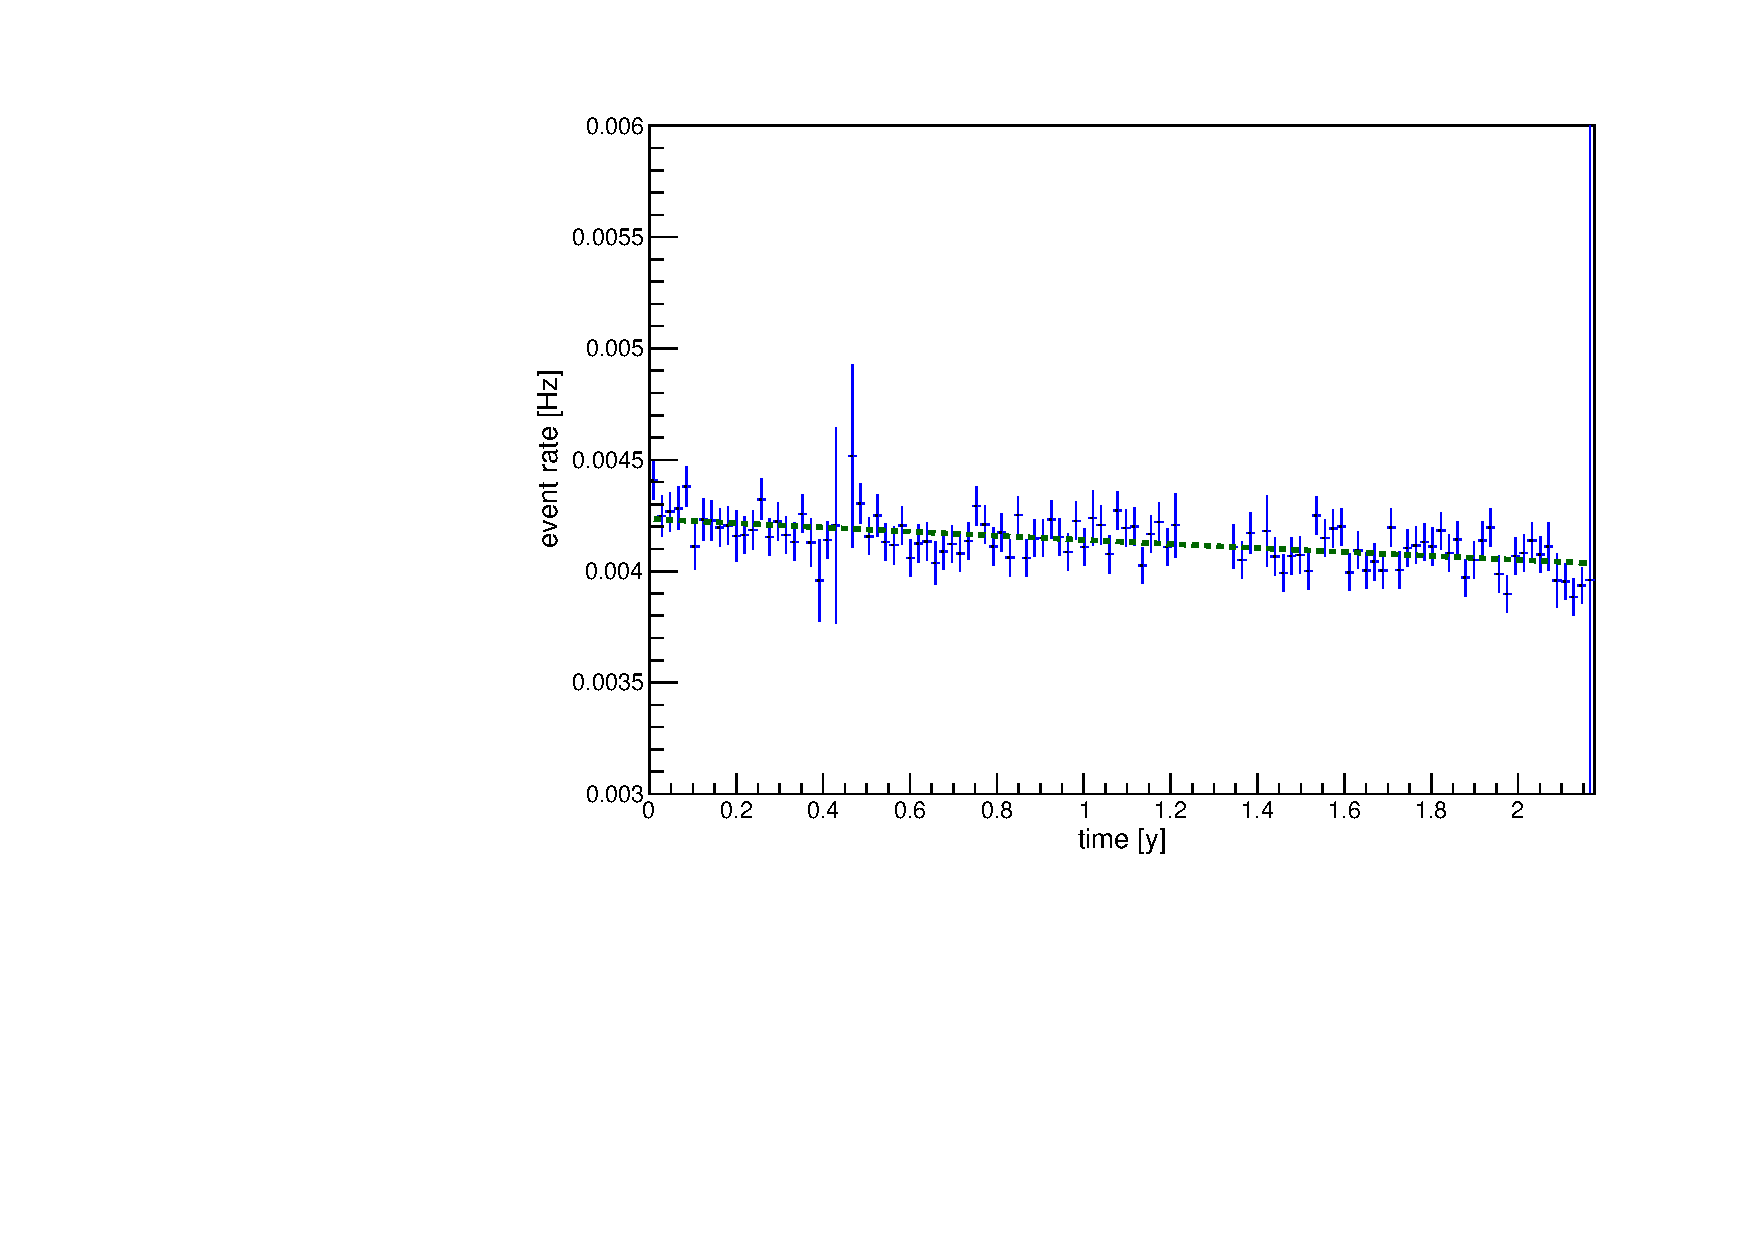
\includegraphics[width=75mm]{./Bilder/doppelt.pdf}
	\fi%
	\caption{double exponential decay fit}
	\label{fig:double}
	\end{minipage}%
	\begin{minipage}{.5\textwidth}
    \centering
    \begin{tabular}{|l|c|}
        \hline
        Name  & Value \\
        \hline
        A     & 0.0010244$\pm$0.000122073 \\
        \hline
        B    & 10.739 \\
        \hline
        C   & 0.00145395$\pm$0.000129916 \\
        \hline
        D  & 32.9 \\
        \hline
        E & 0.00175652$\pm$0.000119112 \\
        \hline
    \end{tabular}
    \captionof{table}{}{Fit parameters of the double exponential decay analysis}
    \label{tab:doubleFitpara}
	\end{minipage}
\end{figure}


In a direct comparison of figure \ref{fig:double} with graph \ref{fig:ChangeInEventRateFit} no real difference can be see.
But when looking at the fit parameters you can see that in this case the \nuc{Ar}{42} exponential fit function has a bigger amplitude than \Kr.
Because the \nuc{K}{42} density is not homogeneously distributed in the liquid argon it is impossible to run a Monte Carlo simulation to again determine a new detector efficiency.
But using the conversation factor determined from the second simulation to make an estimate the respective effective specific activities can be calculated to $(40.4\pm0.59)\frac{\unit{mBq}}{\unit{l}}$ for \Kr and $(57.3\pm0.66)\frac{\unit{mBq}}{\unit{l}}$ for all of the decays resulting from \nuc{Ar}{42}.
These values are both still way to high for what was expected from them.
For the \Kr it is obvious but for \nuc{Ar}{42} the maximum effective specific activity expected to be measured should have only been about one orders of magnitude higher than the actual specific activity of only the \nuc{Ar}{42}.
Due to the fit parameters still generating far too much specific activity for these isotopes shows that other sources of change are still not accounted for.
Nevertheless it has been shown with this fit that \Kr does not contribute solemnly to the change of count rate over time and with this the assumption from before has been shown to be false.
\\

Theoretically it would now still be possible to determine an specific activity of \Kr from plot \ref{fig:ChangeInEventRate} but considerein every individual source of change in count rate.
But because of the higher number of fit parameters that would have to be determined and the relatively large uncertainties in the plot compared to the overall change, it is not difficult to be pessimistic whether this analysis can even make a statement about the specific activity of \Kr.
\\

At the end of this analysis it is again of interest to investigate how the change in the count rate would have looked over time if the specific activities of the WARP or the Darkside experiment had been present.
Again, in the case of the WARP experiment an activity of $(0.16\pm0.13)\frac{\unit{Bq}}{\unit{l}}$ was measured. 
If one would plot its equivalent amplitude in a diagram like Figure \ref{fig:ChangeInEventRateFit} a significant change would have been visible.
On the other hand is the activity in the Darkside experiment with its $(2.8577 \pm 0.18122) \frac{\unit{mBq}}{\unit{l}}$ too small to measure an apparent change over time.
\\

% use fit to calculate the decrease in rate of the signals in range from 200 to 500keV
% from fit and assumption that only Kr85's activity is decreasing one can calculate the specific activity from the amplitude of the fit

% use Volume of LAr-Tank to determine the number of Kr85 and from this the concentration in the argon

\chapter{Summary and Outlook}
\label{sec:ConcAndOutlook}

With the line count rate analysis carried out in this paper it could be shown that the specific activity of \nuc{Kr}{85} in the liquid argon of the GERDA experiment has a value of $(0.508\pm0.0857) \frac{\unit{mBq}}{\unit{l}}$. 
Compared to WARPs $(160\pm130)\frac{\unit{mBq}}{\unit{l}}$ and to Darksides $(2.8577 \pm 0.18122) \frac{\unit{mBq}}{\unit{l}}$ its value is much smaller.
On the other hand, the second attempt to determine a value for the specific activity via the change of count rate over time has failed.
This was due to the falsely made assumption that \Kr is the only isotope in the liquid argon to show significant change in its activity over time.
\\


\backmatter

\bibliography{references}
\bibliographystyle{plain}
\end{document}